% Options for packages loaded elsewhere
\PassOptionsToPackage{unicode}{hyperref}
\PassOptionsToPackage{hyphens}{url}
\PassOptionsToPackage{dvipsnames,svgnames,x11names}{xcolor}
%
\documentclass[
]{scrartcl}

\usepackage{amsmath,amssymb}
\usepackage{iftex}
\ifPDFTeX
  \usepackage[T1]{fontenc}
  \usepackage[utf8]{inputenc}
  \usepackage{textcomp} % provide euro and other symbols
\else % if luatex or xetex
  \usepackage{unicode-math}
  \defaultfontfeatures{Scale=MatchLowercase}
  \defaultfontfeatures[\rmfamily]{Ligatures=TeX,Scale=1}
\fi
\usepackage{lmodern}
\ifPDFTeX\else  
    % xetex/luatex font selection
\fi
% Use upquote if available, for straight quotes in verbatim environments
\IfFileExists{upquote.sty}{\usepackage{upquote}}{}
\IfFileExists{microtype.sty}{% use microtype if available
  \usepackage[]{microtype}
  \UseMicrotypeSet[protrusion]{basicmath} % disable protrusion for tt fonts
}{}
\makeatletter
\@ifundefined{KOMAClassName}{% if non-KOMA class
  \IfFileExists{parskip.sty}{%
    \usepackage{parskip}
  }{% else
    \setlength{\parindent}{0pt}
    \setlength{\parskip}{6pt plus 2pt minus 1pt}}
}{% if KOMA class
  \KOMAoptions{parskip=half}}
\makeatother
\usepackage{xcolor}
\setlength{\emergencystretch}{3em} % prevent overfull lines
\setcounter{secnumdepth}{5}
% Make \paragraph and \subparagraph free-standing
\ifx\paragraph\undefined\else
  \let\oldparagraph\paragraph
  \renewcommand{\paragraph}[1]{\oldparagraph{#1}\mbox{}}
\fi
\ifx\subparagraph\undefined\else
  \let\oldsubparagraph\subparagraph
  \renewcommand{\subparagraph}[1]{\oldsubparagraph{#1}\mbox{}}
\fi

\providecommand{\tightlist}{%
  \setlength{\itemsep}{0pt}\setlength{\parskip}{0pt}}\usepackage{longtable,booktabs,array}
\usepackage{calc} % for calculating minipage widths
% Correct order of tables after \paragraph or \subparagraph
\usepackage{etoolbox}
\makeatletter
\patchcmd\longtable{\par}{\if@noskipsec\mbox{}\fi\par}{}{}
\makeatother
% Allow footnotes in longtable head/foot
\IfFileExists{footnotehyper.sty}{\usepackage{footnotehyper}}{\usepackage{footnote}}
\makesavenoteenv{longtable}
\usepackage{graphicx}
\makeatletter
\def\maxwidth{\ifdim\Gin@nat@width>\linewidth\linewidth\else\Gin@nat@width\fi}
\def\maxheight{\ifdim\Gin@nat@height>\textheight\textheight\else\Gin@nat@height\fi}
\makeatother
% Scale images if necessary, so that they will not overflow the page
% margins by default, and it is still possible to overwrite the defaults
% using explicit options in \includegraphics[width, height, ...]{}
\setkeys{Gin}{width=\maxwidth,height=\maxheight,keepaspectratio}
% Set default figure placement to htbp
\makeatletter
\def\fps@figure{htbp}
\makeatother
\newlength{\cslhangindent}
\setlength{\cslhangindent}{1.5em}
\newlength{\csllabelwidth}
\setlength{\csllabelwidth}{3em}
\newlength{\cslentryspacingunit} % times entry-spacing
\setlength{\cslentryspacingunit}{\parskip}
\newenvironment{CSLReferences}[2] % #1 hanging-ident, #2 entry spacing
 {% don't indent paragraphs
  \setlength{\parindent}{0pt}
  % turn on hanging indent if param 1 is 1
  \ifodd #1
  \let\oldpar\par
  \def\par{\hangindent=\cslhangindent\oldpar}
  \fi
  % set entry spacing
  \setlength{\parskip}{#2\cslentryspacingunit}
 }%
 {}
\usepackage{calc}
\newcommand{\CSLBlock}[1]{#1\hfill\break}
\newcommand{\CSLLeftMargin}[1]{\parbox[t]{\csllabelwidth}{#1}}
\newcommand{\CSLRightInline}[1]{\parbox[t]{\linewidth - \csllabelwidth}{#1}\break}
\newcommand{\CSLIndent}[1]{\hspace{\cslhangindent}#1}

\usepackage{booktabs}
\usepackage{caption}
\usepackage{longtable}
\usepackage{colortbl}
\usepackage{array}
\usepackage{typearea}
\usepackage{lscape}
\usepackage{afterpage}
\usepackage{changepage}
\usepackage{scrlayer-scrpage}
\usepackage{soul}
\usepackage{lastpage}
\lohead{ADVANCE TRAUMA Trial Protocol}
\rohead{ClinicalTrials.gov ID NCT06321419}
\cfoot{\thepage\ of \pageref{LastPage} }
\makeatletter
\makeatother
\makeatletter
\makeatother
\makeatletter
\@ifpackageloaded{caption}{}{\usepackage{caption}}
\AtBeginDocument{%
\ifdefined\contentsname
  \renewcommand*\contentsname{Table of contents}
\else
  \newcommand\contentsname{Table of contents}
\fi
\ifdefined\listfigurename
  \renewcommand*\listfigurename{List of Figures}
\else
  \newcommand\listfigurename{List of Figures}
\fi
\ifdefined\listtablename
  \renewcommand*\listtablename{List of Tables}
\else
  \newcommand\listtablename{List of Tables}
\fi
\ifdefined\figurename
  \renewcommand*\figurename{Figure}
\else
  \newcommand\figurename{Figure}
\fi
\ifdefined\tablename
  \renewcommand*\tablename{Table}
\else
  \newcommand\tablename{Table}
\fi
}
\@ifpackageloaded{float}{}{\usepackage{float}}
\floatstyle{ruled}
\@ifundefined{c@chapter}{\newfloat{codelisting}{h}{lop}}{\newfloat{codelisting}{h}{lop}[chapter]}
\floatname{codelisting}{Listing}
\newcommand*\listoflistings{\listof{codelisting}{List of Listings}}
\makeatother
\makeatletter
\@ifpackageloaded{caption}{}{\usepackage{caption}}
\@ifpackageloaded{subcaption}{}{\usepackage{subcaption}}
\makeatother
\makeatletter
\@ifpackageloaded{tcolorbox}{}{\usepackage[skins,breakable]{tcolorbox}}
\makeatother
\makeatletter
\@ifundefined{shadecolor}{\definecolor{shadecolor}{rgb}{.97, .97, .97}}
\makeatother
\makeatletter
\makeatother
\makeatletter
\makeatother

\usepackage{hyphenat}
\usepackage{ifthen}
\usepackage{calc}
\usepackage{calculator}



\usepackage{graphicx}
\usepackage{geometry}
\usepackage{afterpage}
\usepackage{tikz}
\usetikzlibrary{calc}
\usetikzlibrary{fadings}
\usepackage[pagecolor=none]{pagecolor}


% Set the titlepage font families







% Set the coverpage font families

\ifLuaTeX
  \usepackage{selnolig}  % disable illegal ligatures
\fi
\IfFileExists{bookmark.sty}{\usepackage{bookmark}}{\usepackage{hyperref}}
\IfFileExists{xurl.sty}{\usepackage{xurl}}{} % add URL line breaks if available
\urlstyle{same} % disable monospaced font for URLs
\hypersetup{
  pdftitle={Clinical Trial Protocol},
  pdfauthor={Version 1.2.0, 2024-08-26},
  colorlinks=true,
  linkcolor={blue},
  filecolor={Maroon},
  citecolor={Blue},
  urlcolor={Blue},
  pdfcreator={LaTeX via pandoc}}

\title{Clinical Trial Protocol}
\usepackage{etoolbox}
\makeatletter
\providecommand{\subtitle}[1]{% add subtitle to \maketitle
  \apptocmd{\@title}{\par {\large #1 \par}}{}{}
}
\makeatother
\subtitle{ADVANCE TRAUMA\\
\strut \\
Effects of Advanced Trauma Life Support\textsuperscript{®} Training
Compared to Standard Care on Adult Trauma Patient Outcomes: A Cluster
Randomised Trial}
\author{Version 1.2.0, 2024-08-26}
\date{}

\begin{document}
%%%%% begin titlepage extension code


\begin{titlepage}

%%% TITLE PAGE START

% Set up alignment commands
%Page
\newcommand{\titlepagepagealign}{
\ifthenelse{\equal{center}{right}}{\raggedleft}{}
\ifthenelse{\equal{center}{center}}{\centering}{}
\ifthenelse{\equal{center}{left}}{\raggedright}{}
}


\newcommand{\titleandsubtitle}{
% Title and subtitle
{\fontsize{15}{18.0}\selectfont
{\uppercase{\nohyphens{Clinical Trial Protocol}}}\par
}%

\vspace{\betweentitlesubtitle}
{
\fontsize{20}{24.0}\selectfont
{\bfseries{\nohyphens{ADVANCE TRAUMA\\
\strut \\
Effects of Advanced Trauma Life Support\textsuperscript{®} Training
Compared to Standard Care on Adult Trauma Patient Outcomes: A Cluster
Randomised Trial}}}\par
}}
\newcommand{\titlepagetitleblock}{
\rule{\textwidth}{0.4pt} % Thin horizontal rule
\vspace{0.025\textheight} % Whitespace between the top rules and title

\titleandsubtitle

\vspace{0.025\textheight} 
\rule{0.3\textwidth}{0.4pt} % Short horizontal rule under the title
}
\newcommand{\authorstyle}[1]{{\Large{#1}}}

\newcommand{\affiliationstyle}[1]{{\large{#1}}}

\newcommand{\titlepageauthorblock}{
{\authorstyle{\nohyphens{Version 1.2.0, 2024-08-26}\\}}
}

\newcommand{\titlepageaffiliationblock}{
\hangindent=1em
\hangafter=1
{\affiliationstyle{


\vspace{1\baselineskip} 
}}
}
\newcommand{\headerstyled}{%
{}
}
\newcommand{\footerstyled}{%
{\large{\textsc{}}}
}
\newcommand{\datestyled}{%
{}
}


\newcommand{\titlepageheaderblock}{\headerstyled}

\newcommand{\titlepagefooterblock}{
\footerstyled
}

\newcommand{\titlepagedateblock}{
\datestyled
}

%set up blocks so user can specify order
\newcommand{\titleblock}{\newlength{\betweentitlesubtitle}
\setlength{\betweentitlesubtitle}{\baselineskip}
{

{\titlepagetitleblock}
}

\vspace{0.1\textheight}
}

\newcommand{\authorblock}{{\titlepageauthorblock}

\vspace{2\baselineskip}
}

\newcommand{\affiliationblock}{{\titlepageaffiliationblock}

\vspace{1pt}
}

\newcommand{\logoblock}{}

\newcommand{\footerblock}{}

\newcommand{\dateblock}{}

\newcommand{\headerblock}{}

\thispagestyle{empty} % no page numbers on titlepages


\newlength{\minipagewidth}
\setlength{\minipagewidth}{\textwidth}
\raggedright % single minipage
% [position of box][box height][inner position]{width}
% [s] means stretch out vertically; assuming there is a vfill
\begin{minipage}[b][\textheight][s]{\minipagewidth}
\titlepagepagealign
\titleblock

\authorblock

\vfill

\logoblock

\footerblock
\par

\end{minipage}\ifthenelse{\equal{}{right} \OR \equal{}{leftright} }{
\hspace{\B}
\vrulecode}{}
\clearpage
%%% TITLE PAGE END
\end{titlepage}
\setcounter{page}{1}

%%%%% end titlepage extension code
\ifdefined\Shaded\renewenvironment{Shaded}{\begin{tcolorbox}[boxrule=0pt, interior hidden, sharp corners, breakable, enhanced, frame hidden, borderline west={3pt}{0pt}{shadecolor}]}{\end{tcolorbox}}\fi

\renewcommand*\contentsname{Table of contents}
{
\hypersetup{linkcolor=}
\setcounter{tocdepth}{3}
\tableofcontents
}
\newpage{}

\hypertarget{administrative-information}{%
\section{Administrative information}\label{administrative-information}}

\hypertarget{changelog}{%
\subsection{Changelog}\label{changelog}}

\begin{longtable}[]{@{}
  >{\raggedright\arraybackslash}p{(\columnwidth - 4\tabcolsep) * \real{0.1000}}
  >{\raggedright\arraybackslash}p{(\columnwidth - 4\tabcolsep) * \real{0.1500}}
  >{\raggedright\arraybackslash}p{(\columnwidth - 4\tabcolsep) * \real{0.7500}}@{}}
\toprule\noalign{}
\begin{minipage}[b]{\linewidth}\raggedright
Version
\end{minipage} & \begin{minipage}[b]{\linewidth}\raggedright
Date
\end{minipage} & \begin{minipage}[b]{\linewidth}\raggedright
Details
\end{minipage} \\
\midrule\noalign{}
\endhead
\bottomrule\noalign{}
\endlastfoot
1.3.0 & 2024-11-13 & \begin{minipage}[t]{\linewidth}\raggedright
\begin{itemize}
\tightlist
\item
  Updated names of events in the table of procedures
\item
  Added new references
\item
  Added nested staircase design for measuring adherence, quality of
  life, disability and return to work
\item
  Updated small sample correction to be based on best available evidence
  closer to the time of analysis
\item
  Added contributors
\item
  Removed reassessment of the sample size calculation from the interim
  analysis
\end{itemize}
\end{minipage} \\
1.2.0 & 2024-08-26 & \begin{minipage}[t]{\linewidth}\raggedright
\begin{itemize}
\tightlist
\item
  Added details on measuring ATLS adherence
\item
  Clarified the section describing the consent process
\item
  Fixed minor issues with how the variables were listed
\item
  Indicated non-routinely recorded data in the list of variables
\item
  Added Administrative information section with contributors
\item
  Added CTRI registration number
\end{itemize}
\end{minipage} \\
1.1.0 & 2024-05-09 & Updated the primary outcome to in-hospital
mortality and spelling corrections. The primary outcome was updated
following a voting procedure in the Trial Management Group. \\
\end{longtable}

\hypertarget{study-identifiers}{%
\subsection{Study identifiers}\label{study-identifiers}}

\begin{itemize}
\tightlist
\item
  ClinicalTrials.gov identifier:
  \href{https://clinicaltrials.gov/ct2/show/NCT06321419}{NCT06321419}
\item
  Clinical Trials Registry - India identifier: CTRI/2024/07/071336
\end{itemize}

\hypertarget{contributors}{%
\subsection{Contributors}\label{contributors}}

The following have contributed to the design and implementation of the
trial:

\begin{longtable}[]{@{}
  >{\raggedright\arraybackslash}p{(\columnwidth - 4\tabcolsep) * \real{0.3500}}
  >{\raggedright\arraybackslash}p{(\columnwidth - 4\tabcolsep) * \real{0.4500}}
  >{\raggedright\arraybackslash}p{(\columnwidth - 4\tabcolsep) * \real{0.2000}}@{}}
\toprule\noalign{}
\begin{minipage}[b]{\linewidth}\raggedright
Name and ORCID
\end{minipage} & \begin{minipage}[b]{\linewidth}\raggedright
Affiliation
\end{minipage} & \begin{minipage}[b]{\linewidth}\raggedright
Role
\end{minipage} \\
\midrule\noalign{}
\endhead
\bottomrule\noalign{}
\endlastfoot
Martin Gerdin Wärnberg
\href{https://orcid.org/0000-0001-6069-4794}{
\includegraphics[width=0.16667in,height=0.16667in]{ORCIDiD_icon16x16.png}}
& Karolinska Institutet, Stockholm, Sweden & Principal Investigator, TMG
chair and TT member \\
Girish D Bakhshi
\href{https://orcid.org/0000-0001-9542-4428}{
\includegraphics[width=0.16667in,height=0.16667in]{ORCIDiD_icon16x16.png}}
& Grant Govt. Medical College \& Sir J. J. Group of Hospitals, Mumbai,
India & TMG member \\
Debojit Basak
\href{https://orcid.org/90000-0002-8378-9689}{
\includegraphics[width=0.16667in,height=0.16667in]{ORCIDiD_icon16x16.png}}
& Institute of Post Graduate Medical Education \& Research and Seth
Sukhlal Karnani Memorial Hospital, Kolkata, India & TMG member \\
Abhinav Bassi
\href{https://orcid.org/0000-0003-0750-9179}{
\includegraphics[width=0.16667in,height=0.16667in]{ORCIDiD_icon16x16.png}}
& The George Institute for Global Health, New Delhi, India & TMG and TT
member \\
Johanna Berg
\href{https://orcid.org/0000-0001-7553-7337}{
\includegraphics[width=0.16667in,height=0.16667in]{ORCIDiD_icon16x16.png}}
& Karolinska Institutet, Stockholm, Sweden & TMG member \\
Shamita Chatterjee
\href{https://orcid.org/0000-0002-9460-108X}{
\includegraphics[width=0.16667in,height=0.16667in]{ORCIDiD_icon16x16.png}}
& Institute of Post Graduate Medical Education \& Research and Seth
Sukhlal Karnani Memorial Hospital, Kolkata, India & TMG member \\
Kapil Dev Soni
\href{https://orcid.org/0000-0003-1214-4119}{
\includegraphics[width=0.16667in,height=0.16667in]{ORCIDiD_icon16x16.png}}
& All India Institute of Medical Sciences, New Delhi, India & TMG
member \\
Karla Hemming
\href{https://orcid.org/0000-0002-2226-6550}{
\includegraphics[width=0.16667in,height=0.16667in]{ORCIDiD_icon16x16.png}}
& University of Birmingham, Birmingham, UK & TMG member \\
Vivekanand Jha
\href{https://orcid.org/0000-0002-8015-9470}{
\includegraphics[width=0.16667in,height=0.16667in]{ORCIDiD_icon16x16.png}}
& The George Institute for Global Health, New Delhi, India & TMG
member \\
Jessica Kasza
\href{https://orcid.org/0000-0002-8940-0136}{
\includegraphics[width=0.16667in,height=0.16667in]{ORCIDiD_icon16x16.png}}
& Monash University, Melbourne, Australia & External statistician \\
Monty Khajanchi
\href{https://orcid.org/0000-0002-0898-6391}{
\includegraphics[width=0.16667in,height=0.16667in]{ORCIDiD_icon16x16.png}}
& King Edward Memorial Hospital, Mumbai, India & TMG and TT member \\
James Martin
\href{https://orcid.org/0000-0002-6949-4200}{
\includegraphics[width=0.16667in,height=0.16667in]{ORCIDiD_icon16x16.png}}
& University of Birmingham, Birmingham, UK & External statistician \\
Anurag Mishra
\href{https://orcid.org/0000-0002-2302-0632}{
\includegraphics[width=0.16667in,height=0.16667in]{ORCIDiD_icon16x16.png}}
& Maulana Azad Medical College, New Delhi, India & TMG member \\
Samriddhi Ranjan
\href{https://orcid.org/0000-0002-4277-6662}{
\includegraphics[width=0.16667in,height=0.16667in]{ORCIDiD_icon16x16.png}}
& The George Institute for Global Health, New Delhi, India & TMG and TT
member \\
Anna Olofsson
\href{https://orcid.org/0000-0002-9460-108X}{
\includegraphics[width=0.16667in,height=0.16667in]{ORCIDiD_icon16x16.png}}
& Karolinska Institutet & Trial Statistician, TMG member \\
Nobhojit Roy
\href{https://orcid.org/0000-0003-2022-7416}{
\includegraphics[width=0.16667in,height=0.16667in]{ORCIDiD_icon16x16.png}}
& The George Institute for Global Health, New Delhi, India & TMG and TT
member \\
Rajdeep Singh
\href{https://orcid.org/0000-0001-6593-2624}{
\includegraphics[width=0.16667in,height=0.16667in]{ORCIDiD_icon16x16.png}}
& Maulana Azad Medical College, New Delhi, India & TMG member \\
Lovisa Strömmer
\href{https://orcid.org/0000-0001-5424-7111}{
\includegraphics[width=0.16667in,height=0.16667in]{ORCIDiD_icon16x16.png}}
& Karolinska Institutet, Stockholm, Sweden & TMG member \\
Li Felländer-Tsai
\href{https://orcid.org/0000-0003-0693-6080}{
\includegraphics[width=0.16667in,height=0.16667in]{ORCIDiD_icon16x16.png}}
& Karolinska Institutet, Stockholm, Sweden & TMG member \\
\end{longtable}

Abbreviations: TMG, Trial Management Group; TT, Trial Team.

\newpage{}

\hypertarget{synopsis}{%
\section{Synopsis}\label{synopsis}}

\textbf{Title} Effects of Advanced Trauma Life
Support\textsuperscript{®} Training Compared to Standard Care on Adult
Trauma Patient Outcomes: A Cluster Randomised Trial

\textbf{Rationale} Trauma is a massive global health issue. Many
training programmes have been developed to help physicians in the
initial management of trauma patients. Among these programmes, Advanced
Trauma Life Support\textsuperscript{®} (ATLS\textsuperscript{®}) is the
most popular, having trained over one million physicians worldwide.
Despite its widespread use, there are no controlled trials showing that
ATLS\textsuperscript{®} improves patient outcomes. Multiple systematic
reviews emphasise the need for such trials.

\textbf{Aim} To compare the effects of ATLS\textsuperscript{®} training
with standard care on outcomes in adult trauma patients.

\textbf{Primary Outcome} In-hospital mortality within 30 days of arrival
at the emergency department.

\textbf{Trial Design} Batched stepped-wedge cluster randomised trial in
India.

\textbf{Trial Population} Adult trauma patients presenting to the
emergency department of a participating hospital.

\textbf{Sample Size} 30 clusters and 4320 patients.

\textbf{Eligibility Criteria}

\emph{Hospitals} are secondary or tertiary hospitals in India that admit
or refer/transfer for admission at least 400 patients with trauma per
year.

\emph{Clusters} are one or more units of physicians providing initial
trauma care in the emergency department of tertiary hospitals in India.

\emph{Patients participants} are adult trauma patients who presents to
the emergency department of participating hospitals and are admitted or
transferred for admission.

\textbf{Intervention} The intervention will be ATLS\textsuperscript{®}
training, a proprietary 2.5 day course teaching a standardised approach
to trauma patient care using the concepts of a primary and secondary
survey. Physicians will be trained in an accredited
ATLS\textsuperscript{®} training facility in India.

\textbf{Ethical Considerations} We will use an opt-out consent approach
for collection of routinely recorded data. We will obtain informed
consent for collection of non-routinely recorded data, such as quality
of life and disability outcomes. Patients who are unconscious or lack a
legally authorized representative will be included under a waiver of
informed consent. Note that consent here refers to consent to data
collection.

\textbf{Trial Period} November 2024, to October 2029

\newpage{}

\hypertarget{background-and-rationale}{%
\section{Background and rationale}\label{background-and-rationale}}

Each year, 4.3 million people die from trauma\textsuperscript{1}. Among
people aged 10-24 and 25-49 years trauma is the largest cause of
disability adjusted life years\textsuperscript{2}. Most deaths from
trauma occur within the first 24-48 hours\textsuperscript{3}. Traumatic
brain injury and exsanguination are the most common causes of trauma
deaths\textsuperscript{4,5}. Most preventable trauma deaths are caused
by clinical judgement errors during initial resuscitation or early care
including airway management and haemorrhage control, even though the
deaths occur later during the hospital stay\textsuperscript{4,6}.

Several trauma life support training programmes have been developed to
improve the early management of patients in the hospital by providing a
structured framework for assessment and
treatment\textsuperscript{7--11}. The proprietary Advanced Trauma Life
Support\textsuperscript{®} (ATLS\textsuperscript{®}) is the most
established trauma life support training programme and more than one
million physicians in over 80 countries have been trained in the
programme since the first course in 1978\textsuperscript{12}. In the US
and many other countries training in ATLS\textsuperscript{®} is
virtually mandatory for trauma care physicians\textsuperscript{13}.
Uptake in low- and middle income countries (LMIC) has been slow,
potentially due to high costs\textsuperscript{9}.

There are three randomised studies showing that ATLS\textsuperscript{®}
improves knowledge and clinical skills\textsuperscript{14--16}, but
there are no randomised controlled trials or high-quality
quasi-experimental trials indicating that ATLS\textsuperscript{®}
improves patient outcomes\textsuperscript{7,8,10,11,17}. We conducted an
updated systematic review (unpublished), and estimated a pooled risk
ratio of 0.82 (95\% CI 0.60; 1.11) from ten heterogeneous
(I\textsuperscript{2} 0.91) observational studies on the effect of ATLS
on mortality (see Figure~\ref{fig-forest-plot})\textsuperscript{18--27}.

We conducted a pilot cluster randomised controlled trial
(ClinicalTrials.gov NCT05417243) between April 2022 and February 2023 as
part of our network grant to assess the feasibility of a full scale
trial. We published the protocol for this pilot
study\textsuperscript{28}. Our pilot study enrolled 376 patients from
seven hospitals across India (unpublished data) and shows that it is
feasible to conduct the proposed trial with a high percentage of
patients consenting to out of hospital follow up (78\%), low loss to
follow-up rate (1\%), and low missingness in key variables (mean 0.8\%).

To involve patients and the public in the planning of this trial we
conducted 19 semi-structured interviews with trauma patients,
caregivers, and community representatives (unpublished data). The aim of
these interviews was to understand their views on the trial and
important outcomes and the interviews showed high acceptability of our
research and emphasised the importance of better recovery before
discharge and functional outcomes at and after discharge, including
pain, mobility and self-care activities. The interviews also highlighted
return to work as an important outcome.

\hypertarget{updated-systematic-review}{%
\subsection{Updated systematic review}\label{updated-systematic-review}}

We performed a systematic literature search in the Medline, Embase,
Cochrane, Web of Science, CINAHL and Google Scholar databases (PROSPERO
ID CRD42022373977). The last search was conducted on November 11, 2022.
We developed the search strategy in Medline (Ovid) in collaboration with
librarians at the Karolinska Institutet University Library. We limited
the search to English language articles, searched all databases from
inception, and screened a total of 7896 records. We used a random
effects model to pool estimates across studies.

\begin{figure}

{\centering 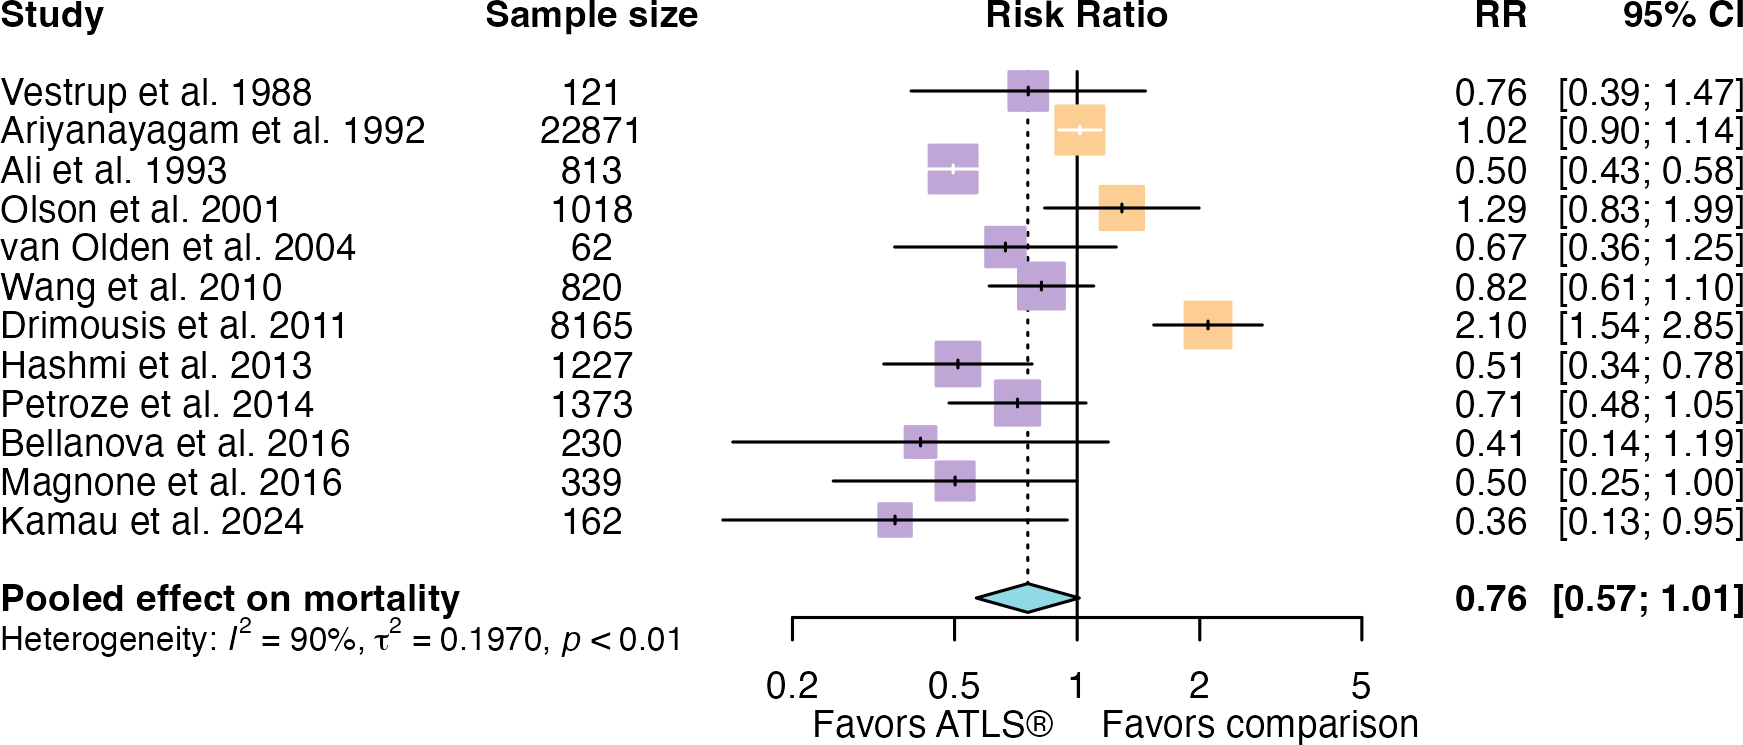
\includegraphics{forest-plot.png}

}

\caption{\label{fig-forest-plot}Summary of the updated system review.
The forest plot shows the effect of ATLS on mortality. Abbreviations:
RR, risk ratio; CI, confidence interval; ATLS, Advanced Trauma Life
Support; I\textsuperscript{2}, heterogeneity.}

\end{figure}

\hypertarget{benefit-risk-evaluation}{%
\section{Benefit-risk evaluation}\label{benefit-risk-evaluation}}

The direct risks includes integrity violations and data leakage. We will
mitigate these risks by employing rigorous data collection and storage
mechanisms. The procedures that we will use to collect data will be
direct observation of care, routine physical examinations,
questionnaires, and extraction of already collected data from patient
records, which are often seen as involving only minimal risk.

The long-term risks of the research and the risk that the research will
be used in detrimental ways are minimal. Our trial will assess the
effect of Advanced Trauma Life Support\textsuperscript{®}
(ATLS\textsuperscript{®}) on patient outcomes. Training in
ATLS\textsuperscript{®} is standard in many health care systems and it
is unlikely that training physicians in this programme induces any harm
to participants.

We consider these risks weighed up by the potential direct benefit for
the participants in the intervention phase, if ATLS\textsuperscript{®}
is found to improve patient outcomes, and by the potential for improved
care for the trauma patient population.

\hypertarget{trial-aim}{%
\section{Trial aim}\label{trial-aim}}

To compare the effects of ATLS\textsuperscript{®} training with standard
care on outcomes in adult trauma patients.

\hypertarget{regulatory-approvals-and-trial-registration}{%
\section{Regulatory approvals and trial
registration}\label{regulatory-approvals-and-trial-registration}}

We will submit this trial to the Health Ministry Screening Committee at
the Indian Council for Medical Research for their approval. We will
apply for ethical approvals from each participating hospital, The George
Institute for Global Health in India and the Swedish Ethical Review
Authority. We will register this trial with Clinical Trials
Registry-India and ClinicalTrials.gov.

\hypertarget{trial-design-and-procedures}{%
\section{Trial design and
procedures}\label{trial-design-and-procedures}}

\hypertarget{overall-trial-design}{%
\subsection{Overall trial design}\label{overall-trial-design}}

We will conduct a batched stepped-wedge cluster randomised controlled
trial (see Figure~\ref{fig-trial-design}). The stepped-wedge trial is a
uni-directional cross-over trial but the time point when clusters
cross-over from standard care to the intervention is
randomised\textsuperscript{29}. Each cluster will be at least one unit
of physicians performing initial resuscitation of trauma patients in the
emergency department of tertiary hospitals in India. The number of units
that we will train in each hospital will depend on the sizes of these
units and the volumes of patients that they see. If more than one unit
is trained in the same hospital these units will be considered one unit
for the purpose of randomisation. We choose this approach for two
reasons: 1) it will not be logistically or financially feasible to train
all physician in a given hospital; and 2) we need to balance cluster
size with the number of clusters. We will conduct this trial in India
because physicians providing initial trauma care in India are so far not
routinely trained in ATLS\textsuperscript{®} or similar programmes.

We will roll out the interventions to 30 clusters over six batches, so
there will be five clusters in each batch. The clusters in each batch
will be randomised to one of five implementation sequences, with one
hospital randomised to each implementation sequence. All clusters will
transition through three phases, first a standard care phase, then a one
month transition phase during which the training is delivered, and
finally an intervention phase, for a total of 13 months. The
implementation sequence determines how long the phases of standard care
and intervention are. Patient participants will be followed up for a
total of three months.

\hypertarget{design-justification}{%
\subsection{Design justification}\label{design-justification}}

We use the cluster randomised design because the intervention cannot be
randomised at the individual patient level. We use the stepped-wedge
design for two reasons. First, this design is statistically more
efficient than the parallel cluster design when the number of clusters
is limited\textsuperscript{30}. In this trial, the number of clusters is
limited because of the costs associated with ATLS\textsuperscript{®}
training and the available slots for ATLS\textsuperscript{®} training in
India. Second, the stepped-wedge design is likely to enhance
participation and engagement because all clusters receive the
intervention. The batched stepped-wedge design further improves
feasibility as it does not require all clusters to start at the same
time, and it is robust to potential delays in cluster
recruitment\textsuperscript{31}.

\begin{figure}

{\centering 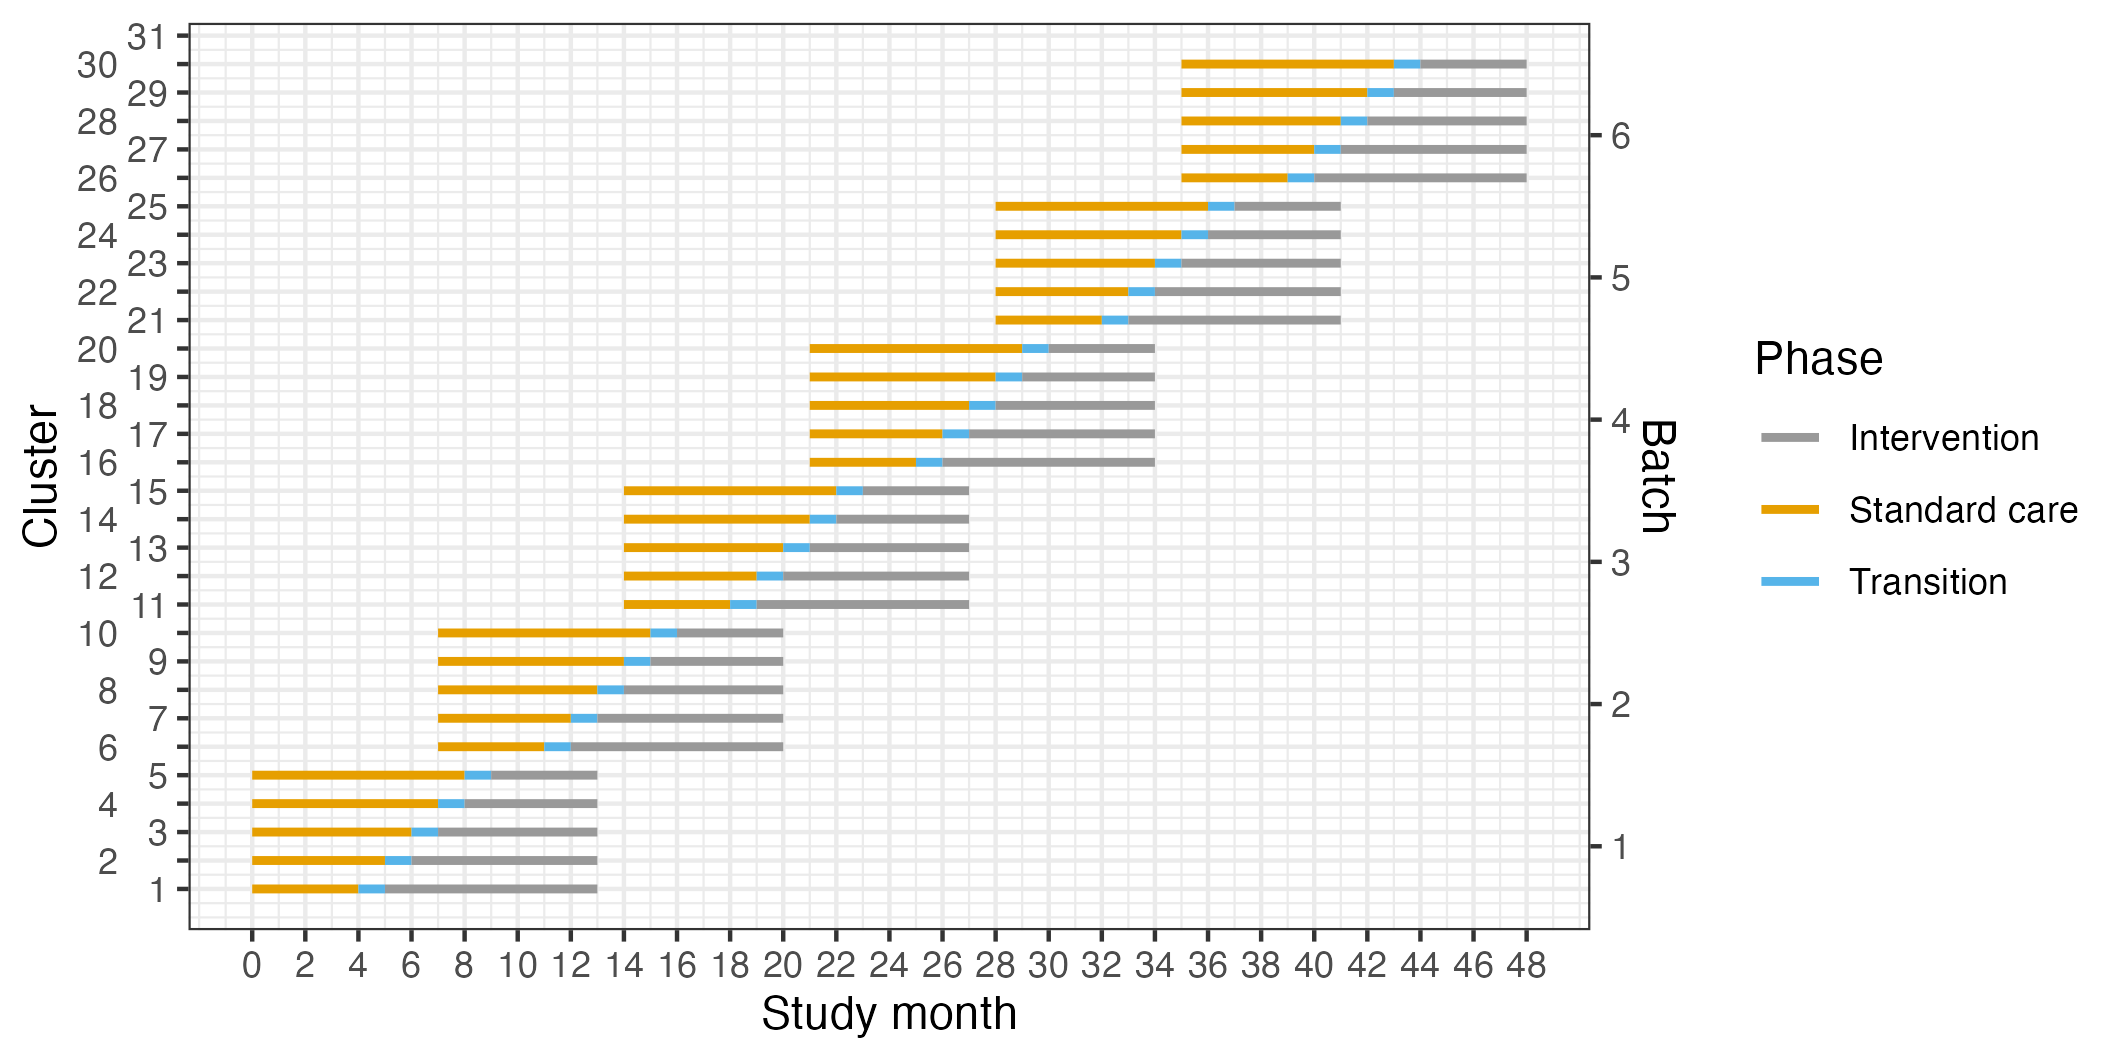
\includegraphics{trial-design-figure-30-clusters-5-sequences-6-batches-6-batches-overlap-4-min-standard-care-4-min-intervention-1-transition-months-0-transition-overlap.png}

}

\caption{\label{fig-trial-design}Trial design. Lines represent the
duration of patient enrolment across clusters and phases. Clusters will
be sequentially allocated to a batch based on when they enter the study.
Within each batch clusters will then be randomised to an intervention
implementation sequence.}

\end{figure}

\hypertarget{eligibility-criteria}{%
\subsection{Eligibility criteria}\label{eligibility-criteria}}

Our trial include eligibility criteria on three levels: hospitals,
clusters and patient participants. We include eligibility on both the
hospital and cluster level to facilitate the screening process.

\hypertarget{hospital-selection}{%
\subsection{Hospital selection}\label{hospital-selection}}

Hospitals will be secondary or tertiary hospitals providing trauma care
in India. Hospital will be the unit of randomisation.

\hypertarget{inclusions-criteria}{%
\subsubsection{Inclusions criteria}\label{inclusions-criteria}}

\textbf{Hospitals} must meet the following criteria:

\begin{itemize}
\tightlist
\item
  admit or refer/transfer for admission at least 400 patients with
  trauma per year or 35 patients with trauma per month for at least the
  last six months;
\item
  provide surgical and orthopaedic emergency services around the clock;
  and
\item
  have at most 25\% of physicians providing initial trauma care trained
  in a formalised trauma life support training programme, like
  ATLS\textsuperscript{®} or Primary Trauma Care (PTC).
\end{itemize}

\hypertarget{exclusion-criteria}{%
\subsubsection{Exclusion criteria}\label{exclusion-criteria}}

\textbf{Hospitals} are excluded if they meet any of the following
criteria:

\begin{itemize}
\tightlist
\item
  the hospital of the cluster implements a formalised trauma life
  support training programme \footnote{These include but are not limited
    to the National Emergency Life Support (NELS) programme, the Basic
    Trauma Life Support (BTLS) programme, the Pre-Hospital Trauma Life
    Support (PHTLS) programme, the Trauma Nursing Core Course (TNCC) and
    the Advanced Trauma Care for Nurses (ATCN) programme.} during the
  trial period; or
\item
  the hospital of the cluster plan to implement or implements other
  major interventions\footnote{These include but are not limited to
    implementing of a trauma team approach, opening a trauma centre and
    implementing a trauma quality improvement programme.} that affects
  trauma care during the trial period.
\end{itemize}

\hypertarget{screening}{%
\subsubsection{Screening}\label{screening}}

The trial management group will compile a list of hospitals with
potentially eligible clusters and reach out to them to assess their
interest in participating in the trial. We will then screen hospitals
for eligibility based on the criteria above, using a two-step procedure.
First, we will approach hospitals to complete an initial hospital
screening instrument (see Appendix
Section~\ref{sec-appendix-hospital-screening-instrument}). We will then
discuss each eligible hospital individually in the Trial Management
Group before deciding whether to include it in the trial. We have this
discussion because we strive to include hospitals that to a large extent
conducts primary resuscitation of trauma patients, rather than hospitals
that primarily receives transferred patients from other hospitals, but
this is difficult to formalise in the eligibility criteria. We will then
perform a more in-depth interview with selected hospitals (See Appendix
Section~\ref{sec-appendix-hospital-screening-interview-instrument}). To
avoid excluding centres we will also discuss plans to implement other
potentially competing interventions during the trial period, and take
these plans into account when assigning clusters to batches. For
example, we are aware of the ongoing implementation of the National
Emergency Life Support (NELS) programme in India, and will therefore not
include hospitals that plan to implement this programme during the trial
period. All screening steps and decisions will be logged using
REDCap\textsuperscript{32,33}.

\hypertarget{cluster-selection}{%
\subsection{Cluster selection}\label{cluster-selection}}

Clusters are one or more units of physicians providing initial trauma
care in the emergency department of secondary or tertiary hospitals in
India. These units already exist in the hospitals and rotate through the
emergency department on specific days of the week.

\hypertarget{inclusion-criteria}{%
\subsubsection{Inclusion criteria}\label{inclusion-criteria}}

\textbf{Clusters} must meet the following criteria:

\begin{itemize}
\tightlist
\item
  admits or refers/transfers for admission at least 12 patients with
  trauma per month for at least the last six months; and
\item
  no more than 25\% of physicians providing initial trauma care trained
  in a formalised trauma life support training programme.
\end{itemize}

\hypertarget{screening-1}{%
\subsubsection{Screening}\label{screening-1}}

The screening of clusters is part of the hospital screening process.

\hypertarget{patient-participants-selection}{%
\subsection{Patient participants
selection}\label{patient-participants-selection}}

Patient participants are adult trauma patients who presents to the
emergency department of participating hospitals and are admitted or
transferred for admission.

\hypertarget{inclusion-criteria-1}{%
\subsubsection{Inclusion criteria}\label{inclusion-criteria-1}}

\textbf{Patients participants} must meet the following criteria:

\begin{itemize}
\tightlist
\item
  age of at least 15 years;
\item
  trauma occurred less than 48 hours before arrival at the hospital;
\item
  present to the emergency department of participating hospitals, with a
  history of trauma defined as having any of the reasons listed in the
  International Classification of Diseases chapter XX as the reason for
  presenting;
\item
  admitted, or died between arrival at the hospital and admission, or
  referred/transferred from the emergency department of a participating
  hospital to another hospital for admission; and
\item
  managed by a participating cluster in the emergency department.
\end{itemize}

\hypertarget{exclusion-criteria-1}{%
\subsubsection{Exclusion criteria}\label{exclusion-criteria-1}}

\textbf{Patients participants} are excluded if they meet the following
criteria:

\begin{itemize}
\tightlist
\item
  present with isolated limb injuries; or
\item
  are directly admitted to a ward without being seen by a physician in
  the emergency department.
\end{itemize}

\hypertarget{screening-2}{%
\subsubsection{Screening}\label{screening-2}}

Clinical research coordinators will screen patient participants either
as they arrive to the emergency department or using emergency department
registers. The patients or their representatives will receive written
information about the study before they are discharged, including about
their right to opt out at any time before final analysis. Phone numbers
for out of hospital follow up will be extracted from the emergency
department registers, and will be securely held only by the clinical
research coordinators at each sites.

\hypertarget{withdrawal-criteria}{%
\subsubsection{Withdrawal criteria}\label{withdrawal-criteria}}

Patient participants can choose to withdraw their consent for collection
of non-routinely recorded data at any time before the final analysis. If
they withdraw their consent for this data collection the clinical
research coordinator will not collect any more of this data, which also
means that no further follow-ups will be conducted. They can also choose
to have the data already collected about them removed from the trial at
any time before final analysis of the data. Withdrawal of consent or
removal of data from the trial will not affect their care in any way. If
the patient participant withdraws consent, follow-up of this participant
will be performed according to the participating hospitals routine.

\hypertarget{procedures}{%
\subsection{Procedures}\label{procedures}}

Table~\ref{tbl-procedures-baseline} shows an overview of trial
procedures before and during patient admission, and
Table~\ref{tbl-procedures-followup} shows an overview of trial follow-up
procedures. Clinical research coordinators will follow up patients daily
until discharge to capture injury information. They will also follow up
patients at 24 hours, 30 days and 90 days after arrival to the emergency
department to capture mortality outcomes, and at 30 days and 90 days
after arrival to the emergency department to capture functional outcomes
and return to work. If patient participants are discharged before any of
these follow-up time points, clinical research coordinators will follow
up patients by phone.

\begingroup
\fontsize{10pt}{11pt}\selectfont
\addtolength{\tabcolsep}{-3pt}

\hypertarget{tbl-procedures-baseline}{}
\setlength{\LTpost}{0mm}
\begin{longtable}{lllll}
\caption{\label{tbl-procedures-baseline}Overview of trial procedures before and during patient admission }\tabularnewline

\toprule
Procedure & Screening & Consenting & Initial assessment & In-hospital care \\ 
\midrule\addlinespace[2.5pt]
Eligibility criteria & √ &  &  &  \\ 
Study information\textsuperscript{\textit{1}} &  & √ &  &  \\ 
Informed consent\textsuperscript{\textit{1}} &  & √ &  &  \\ 
Baseline data collection &  &  & √ &  \\ 
Prehospital data collection &  &  & √ &  \\ 
ATLS adherence\textsuperscript{\textit{2}} &  &  & √ &  \\ 
ED data collection\textsuperscript{\textit{3}} &  &  & √ &  \\ 
Hospital data collection &  &  &  & √ \\ 
Surgery data collection &  &  &  & √ \\ 
Imaging data collection &  &  &  & √ \\ 
Transfusion data collection &  &  &  & √ \\ 
Injury data collection &  &  &  & √ \\ 
Mortality data collection &  &  &  & √ \\ 
Assessment of safety events &  &  &  & √ \\ 
\bottomrule
\end{longtable}
\begin{minipage}{\linewidth}
\textsuperscript{\textit{1}}Clinical research coordinators will inform patient participants about the study, including that they are free to withdraw their data from the study at any time, and approach them for informed consent for collection of non-routinely recorded data in person or telephonically.\\
\textsuperscript{\textit{2}}ATLS adherence will be assessed by observing the care provided to a random sample of patient participants.\\
\textsuperscript{\textit{3}}Emergency Department\\
\end{minipage}

\endgroup

\begingroup
\fontsize{10pt}{11pt}\selectfont
\addtolength{\tabcolsep}{-3pt}

\hypertarget{tbl-procedures-followup}{}
\setlength{\LTpost}{0mm}
\begin{longtable}{llll}
\caption{\label{tbl-procedures-followup}Overview of trial follow-up procedures }\tabularnewline

\toprule
Procedure & Within 7 days of discharge & 30 days & 90 days \\ 
\midrule\addlinespace[2.5pt]
Mortality data collection\textsuperscript{\textit{1}} & √ & √ & √ \\ 
EQ-5D/WHODAS & √ & √ & √ \\ 
Return to work &  & √ & √ \\ 
End of study &  &  & √ \\ 
\bottomrule
\end{longtable}
\begin{minipage}{\linewidth}
\textsuperscript{\textit{1}}Will be ascertained daily from when the patient participant arrive to hospital until they leave the hospital, are discharged or die.\\
\end{minipage}

\endgroup

\hypertarget{biological-sampling-procedures}{%
\subsection{Biological sampling
procedures}\label{biological-sampling-procedures}}

This trial does not include biological sampling.

\hypertarget{end-of-trial}{%
\subsection{End of trial}\label{end-of-trial}}

The trial ends when the last patient participant has completed the last
follow-up. The trial may be prematurely terminated if it this is
necessary for safety reasons affecting the risk-benefit balance or if
the recruitment of subjects cannot be met within reasonable time limits.
If the trial is prematurely terminated or suspended, the investigator
should immediately inform the subjects about this and ensure appropriate
treatment and follow-up. Decisions on premature termination are taken by
the joint Trial Steering and Data Monitoring Committee and Trial
Management Group.

\hypertarget{intervention-and-control-treatment}{%
\subsection{Intervention and control
treatment}\label{intervention-and-control-treatment}}

The intervention will be ATLS\textsuperscript{®} training. The control
will be standard care, meaning no formal trauma life support training.
We will train the physicians that initially resuscitate and provide
trauma care during the first hour after patient arrival at the emergency
department. These physicians can be casualty medical officers, surgical
residents, or emergency medicine residents, depending on the setup at
each participating centre. The training will occur during the transition
phase in each cluster. Our experience from our pilot study is that study
sites adhere to the training slot alloted to them through the trial, so
we judge the risk of clusters implementing ATLS\textsuperscript{®}
before their randomised implementation sequence as very low.

We will train the number units of physicians needed to reach the
required patient sample size, but estimate that this will require
training an average of ten physicians per hospital, which on average
should be mean that we can train one to two units per hospital. This is
possible because many hospitals in India organise physicians staffing
their emergency departments in units, and the physicians in the same
unit work together in the emergency department on the same days of the
week. We will therefore collect data only on the days when these units
work. The units selected to constitute a cluster from each hospital will
be a convenience sample out of all eligible units in those hospitals.

\textbf{Advanced Trauma Life Support\textsuperscript{®}
(ATLS\textsuperscript{®})\textsuperscript{12}} is a proprietary 2.5 day
course teaching a standardised approach to trauma patient care using the
concepts of a primary and secondary survey. The programme was developed
by the Committee of Trauma of the American College of Surgeons. The
course includes intial treatment and resuscitation, triage and
interfacility transfers. Leaning is based on practical scenario-driven
skill stations, lectures and includes a final performance proficiency
evaluation. Physicians will be trained in an accredited
ATLS\textsuperscript{®} training facility in India. We will assess
adherence to ATLS principles before and after implementing ATLS
training.

\textbf{Standard care} varies across hospitals in India, but trauma
patients are initially managed by casualty medical officers, surgical
residents, or emergency medicine residents. They are mainly first- or
second-year residents who resuscitate patients, perform interventions
and refer patients for imaging or other investigations. Compared with
other settings where a trauma team approach is adopted, nurses and other
healthcare professionals are only involved to a limited extent during
the initial management.

\hypertarget{description-of-investigational-medicinal-products}{%
\subsubsection{Description of investigational medicinal
products}\label{description-of-investigational-medicinal-products}}

This trial does not include any investigational medicinal products.

\hypertarget{auxiliary-medicinal-products}{%
\subsubsection{Auxiliary medicinal
products}\label{auxiliary-medicinal-products}}

This trial does not include any auxiliary medicinal products.

\hypertarget{concomitant-use-of-other-medications-or-treatments}{%
\subsubsection{Concomitant use of other medications or
treatments}\label{concomitant-use-of-other-medications-or-treatments}}

Other than implementing another formalised trauma life support training
programme or other major interventions to change the care of trauma
patients as specified in the exclusion criteria, concomitant use of
other medications and treatments may be provided at the discretion of
the investigators and will not be considered an exclusion criterion.

\hypertarget{randomisation}{%
\subsection{Randomisation}\label{randomisation}}

We will assign clusters to batches as they are found to be eligible and
receive ethical approval. Batches will include clusters from hospitals
in different regions to optimize trial logistics. We will randomise the
clusters alloted to each batch to the different intervention
implementation sequences within that batch\footnote{Randomisation will
  be done using bespoke code from previous trials.}. We will balance the
randomisation within each batch on cluster size, defined as monthly
volume of eligible patient participants, using covariate constrained
randomisation. The cluster sizes are expected to vary between 12 and 20
patients per month, based on our previous experiences. We will conceal
the randomisation order for as long as it is logistically possible,
considering that arrangements for sending physicians to
ATLS\textsuperscript{®} training need to be made in advance.

\hypertarget{blinding}{%
\subsection{Blinding}\label{blinding}}

It is not possible to blind a stepped-wedge trial, because all clusters
receive the intervention.

\hypertarget{treatment-after-trial-end}{%
\subsection{Treatment after trial end}\label{treatment-after-trial-end}}

When the trial ends, the intervention will have been implemented in all
clusters.

\hypertarget{outcomes}{%
\subsection{Outcomes}\label{outcomes}}

\hypertarget{primary-outcome}{%
\subsubsection{Primary outcome}\label{primary-outcome}}

The primary outcome will be in-hospital mortality within 30 days of
arrival at the emergency department. Clinical research coordinators will
extract information on death from patient hospital records. If the
patient has been transferred to another hospital, the clinical research
coordinators will collect data on this outcome by calling the patient or
a patient representative, or by contacting the hospital to which the
patient was transferred. Data on this outcome will be collected
continuously during the trial.

\hypertarget{secondary-outcomes}{%
\subsubsection{Secondary outcomes}\label{secondary-outcomes}}

\begin{itemize}
\tightlist
\item
  All cause mortality within 24 hours, 30 days and three months of
  arrival at the emergency department. Data on this outcome will be
  collected in the same way as for the primary outcome.
\item
  Length of emergency department stay. Data on this outcome will be
  collected from patient hospital records.
\item
  Length of hospital stay. Data on this outcome will be collected from
  patient hospital records.
\item
  Intensive care unit admission. Data on this outcome will be collected
  from patient hospital records.
\item
  Length of intensive care unit stay. Data on this outcome will be
  collected from patient hospital records.
\item
  Adherence to ATLS\textsuperscript{®} principles during initial patient
  resuscitation, up to one hour after the physician has first seen the
  patient. This assessment will be done using a 14 item checklist
  covering the key steps of the ATLS\textsuperscript{®} primary
  survey,which was modelled based on previous work on
  ATLS\textsuperscript{®} adherence\textsuperscript{34}. We will
  consider completion of all 14 steps as 100\% adherence. We will
  collect this data by observing the care of a random sample of
  patients. The sampling will be designed as a nested staircase design.
  The clinical research coordinators collecting the data will be trained
  by participating in an ATLS\textsuperscript{®} course as observers,
  prior to the start of the trial.
\item
  Quality of life within seven days of discharge, and at 30 days and
  three months of arrival at the emergency department, measured by the
  official and validated translations of the EQ5D3L. Data on this
  outcome will be collected in person if the patient is still in
  hospital, or by phone if the patient has been discharged. We will
  collect this data using a nested staircase design.
\item
  Disability within seven days of discharge, and at 30 days and three
  months of arrival at the emergency department, assessed using the WHO
  Disability Assessment Schedule 2.0 (WHODAS 2.0). Data on this outcome
  will be collected in person if the patient is still in hospital, or by
  phone if the patient has been discharged. This data will also be
  collected using a nested staircase design.
\item
  Return to work at 30 days and three months after arrival at the
  emergency department. Data on this outcome will be collected in person
  if the patient is still in hospital, or by phone if the patient has
  been discharged. This data will also be collected using a nested
  staircase design.
\end{itemize}

\hypertarget{handling-of-adverse-and-safety-events}{%
\subsection{Handling of adverse and safety
events}\label{handling-of-adverse-and-safety-events}}

\hypertarget{definitions}{%
\subsubsection{Definitions}\label{definitions}}

\hypertarget{adverse-event}{%
\paragraph{Adverse event}\label{adverse-event}}

Any untoward medical occurrence in a clinical trial subject and, which
does not necessarily have a causal relationship with the treatment, can
be an unfavorable and unintended sign (including an abnormal laboratory
discovery), symptom or disease temporally associated with the inclusion
in the trial, whether or not related to the trial.

\hypertarget{serious-adverse-event}{%
\paragraph{Serious adverse event}\label{serious-adverse-event}}

Any untoward medical occurrence in a trial participant that:

\begin{itemize}
\tightlist
\item
  leads to death
\item
  is life-threatening
\item
  requires inpatient hospitalization or prolongation of existing
  hospitalization
\item
  results in persistent or significant disability or incapacity
\item
  results in a congenital anomaly/malformation
\end{itemize}

\hypertarget{safety-event}{%
\paragraph{Safety event}\label{safety-event}}

Any unexpected serious complication that might occur as a consequence of
the trial and that are not part of the natural history of trauma.

\hypertarget{reporting-and-assessment-of-adverse-and-safety-events}{%
\subsubsection{Reporting and assessment of adverse and safety
events}\label{reporting-and-assessment-of-adverse-and-safety-events}}

In alignment with other current trials including critically ill
patients\textsuperscript{35}, we will not collect adverse events or
serious adverse events, because many of these events are expected in
this patient population and we already collect many of these events, for
example mortality, as part of our outcomes.

We will only report safety events, if they are life-threatening, prolong
hospitalisation or result in meaningful harm to the participant. We
cannot pre-define a comprehensive list of events that can be considered
safety events, but will actively assess the presence of the following
safety events:

\begin{itemize}
\tightlist
\item
  Prolonged mechanical ventilation (\textgreater{} 7 days)
\item
  Initiation of renal replacement therapy
\item
  Prolonged (\textgreater{} 2 days) or renewed (restart after at least 2
  days without) use of vasopressors such as norepinephrine or
  vasopressin
\end{itemize}

These events are considered safety events because they suggest
pulmonary, renal, septic or bleeding complications and an increase in
their occurrence following ATLS\textsuperscript{®} training could
indicate that the intervention is harmful. These events therefore need
to be tracked during the standard care phase as well as the intervention
phase, but will only be considered indicative of harm related to the
intervention if they occur more often during the intervention phase than
during the standard care phase.

We will also report any other safety events that we identify during the
trial, and the reporting of such will have to be based on the intuition
of the clinical research coordinators and local investigators. Examples
of such safety events could include missed injuries or missed
investigations, which could be suspected if certain injuries or
investigations were identified or conducted more often during the
standard care phase than during the intervention phase.

All safety events will be recorded in the Case Record Form (CRF) and
reported to the trial management team within 24 hours of its occurrence.
The trial management team will then assess if the event can be
considered related to the trial or the intervention within 24 hours of
it being reported. Events that are considered probably related will be
reported immediately to the joint Trial Steering and Data Monitoring
Committee.

\hypertarget{follow-up-of-safety-events}{%
\subsubsection{Follow up of safety
events}\label{follow-up-of-safety-events}}

All safety events should be followed up by the local investigator until
they are fully evaluated.

\hypertarget{statistics}{%
\subsection{Statistics}\label{statistics}}

\hypertarget{general-principles}{%
\subsubsection{General principles}\label{general-principles}}

We will conduct all analysis by modified intention to treat. Clusters
and observations within clusters will be considered exposed to the
intervention after the date at which the cluster was scheduled to
transition. All data will be included with the exception of the
transition phases. We will not adjust for multiplicity of analyses
because none of the secondary outcomes will be singularly more
important. However, all secondary outcomes will be interpreted with due
consideration for how all are affected by the intervention without
putting any undue emphasis on a single outcome that might be
statistically significant but where all others appear to have remained
unchanged.

We will use a two-sided significance level of 5\% and estimate 95\%
confidence intervals. The primary subgroup analyses will be based on
geographical region because demonstrating the consistency of any effect
across multiple regions will enhance the generalisibility of the
results\footnote{\textbf{Note:} Batches will not be based on regions
  because it will be logistically more feasible to include clusters from
  different regions in each batch.}. Additional subgroup analyses will
include age across the groups older adolescents (15-19 years), young
adults (20-24 years), adults (25-59 years), and older adults (60 years
and older)\textsuperscript{36}; sex; and the clinical cohorts blunt
multisytem trauma, penetrating trauma, and severe isolated traumatic
brain injury.

\hypertarget{analysis-models}{%
\subsubsection{Analysis models}\label{analysis-models}}

There are a number of requirements for the analysis model. Firstly, all
analysis will consider the clustered nature of the design. Secondly, as
the trial has only 30 clusters, it will be essential that the model
allows for a correction due to the small number of clusters. Thirdly, as
the design is a stepped-wedge study, we will adjust for temporal
confounding using categorical effects for period of the study (month).
Full details on how each of these will be undertaken, with justification
is provided below\textsuperscript{37}.

For binary outcomes, a mixed effects binomial regression with a logit
link will be used to estimate the odds ratio; and a binomial model with
identity link used to estimate the risk difference. These models will be
fitted using residual pseudo-likelihood estimation based on
linearization with subject-specific expansion (RSPL). If the binomial
model with the identity link does not converge then only a odds ratio
will be reported.

We will include fixed effects for period and a fixed effect for
intervention exposure. The primary analysis will allow for clustering by
as a random cluster and random cluster by period effect. To correct the
potential inflation of the type I error rate due to small number of
clusters, a correction for a small number of clusters will be applied,
but the correction that will be selected will be based on the best
available evidence available closer to the time, and it may differ for
the outcomes collected via the complete and incomplete designs. In a
sensitivity analysis we will explore if models with more complicated
correlation structures are a better fit to the data. These models are
not being used as our primary analysis models as there is limited
understanding as to when such models will converge and how to choose
between the various different correlation structures which might be
plausible.

To this end we will additionally fit generalised linear mixed models
(with same link functions and fixed effects as described above) to
include a discrete time decay correlation structure including a random
cluster effect with auto-regressive structure (AR(1)). To allow for the
randomisation by batches, a different secular trend will be included for
each batch (interaction between batch and period). For continuous, count
and prevalence outcomes similar model-based approaches will be used but
with appropriate links and distribution functions, using transformations
where appropriate.

\hypertarget{additional-sensitivity-analyses}{%
\subsubsection{Additional sensitivity
analyses}\label{additional-sensitivity-analyses}}

To additionally explore if the fixed period effect is both parsimonious
and adequate to represent the extent of any underlying secular trend, we
will model the time effect using a spline function. Models will also be
extended to include random cluster by intervention effects (with a
non-zero covariance term) to examine if results are sensitive to the
assumption of no intervention by cluster interaction. Models will also
be extended to include an interaction between treatment and number of
periods since first treated, to examine if there is any indication of a
relationship between duration of exposure to the intervention and
outcomes.

This will allow us to different lag effects (whereby it takes time for
the intervention to become embedded within the culture before its impact
can properly start to be realised); as well as weaning effects (whereby
the effect of the intervention starts to decrease -- or fade). This type
of analysis attempts to disentangle how some clusters end up having a
long exposure to the intervention and others have a much shorter
exposure time. A fully adjusted covariate analysis will additionally
adjust for a set of pre-specified individual-level covariates of known
prognostic importance.

\hypertarget{estimation-and-reporting-of-within-cluster-correlations}{%
\subsubsection{Estimation and reporting of within cluster
correlations}\label{estimation-and-reporting-of-within-cluster-correlations}}

We will report time adjusted within-cluster correlations for all
outcomes with 95\% confidence intervals. We will report correlations
from the different assumed correlation structures (so we will report
intra-cluster correlations (ICC); within and between-period
correlations; and within-period correlations and exponential decay). As
well as reporting correlations we will additionally report all variance
components. For all outcomes we will report correlations on the latent
scale (i.e.~proportions scale for binary outcomes) as is appropriate to
inform future sample size calculations.

\hypertarget{sample-size-calculations}{%
\subsubsection{Sample size
calculations}\label{sample-size-calculations}}

With 30 clusters across 6 batches and a total sample size of 4320 our
study has \textasciitilde90\% power across different combinations of
cluster autocorrelations (CAC) and intra-cluster correlations (ICC) to
detect a reduction in the primary outcome of in-hospital mortality
within 30 days from 20\% under standard care to 15\% after
ATLS\textsuperscript{®} training (see Figure~\ref{fig-power-curves}).
This effect is a conservative estimate and the reduction equals a risk
ratio of 0.75, which would be clinically important while also being
consistent with our pilot study and updated systematic review. We
allowed for the clustered design and assumed an ICC of 0.02, but
considered sensitivity across the range
0.01-0.05\textsuperscript{38,39}, and a CAC of 0.9 but considered
sensitivity across the range 0.8-1.0, based on our pilot study and
current guidance\textsuperscript{40--42}. We included the CAC to allow
for variation in clustering over time. We assume that each cluster will
contribute approximately 12 observations per month to the analysis,
based on our previous work.

\begin{figure}

{\centering 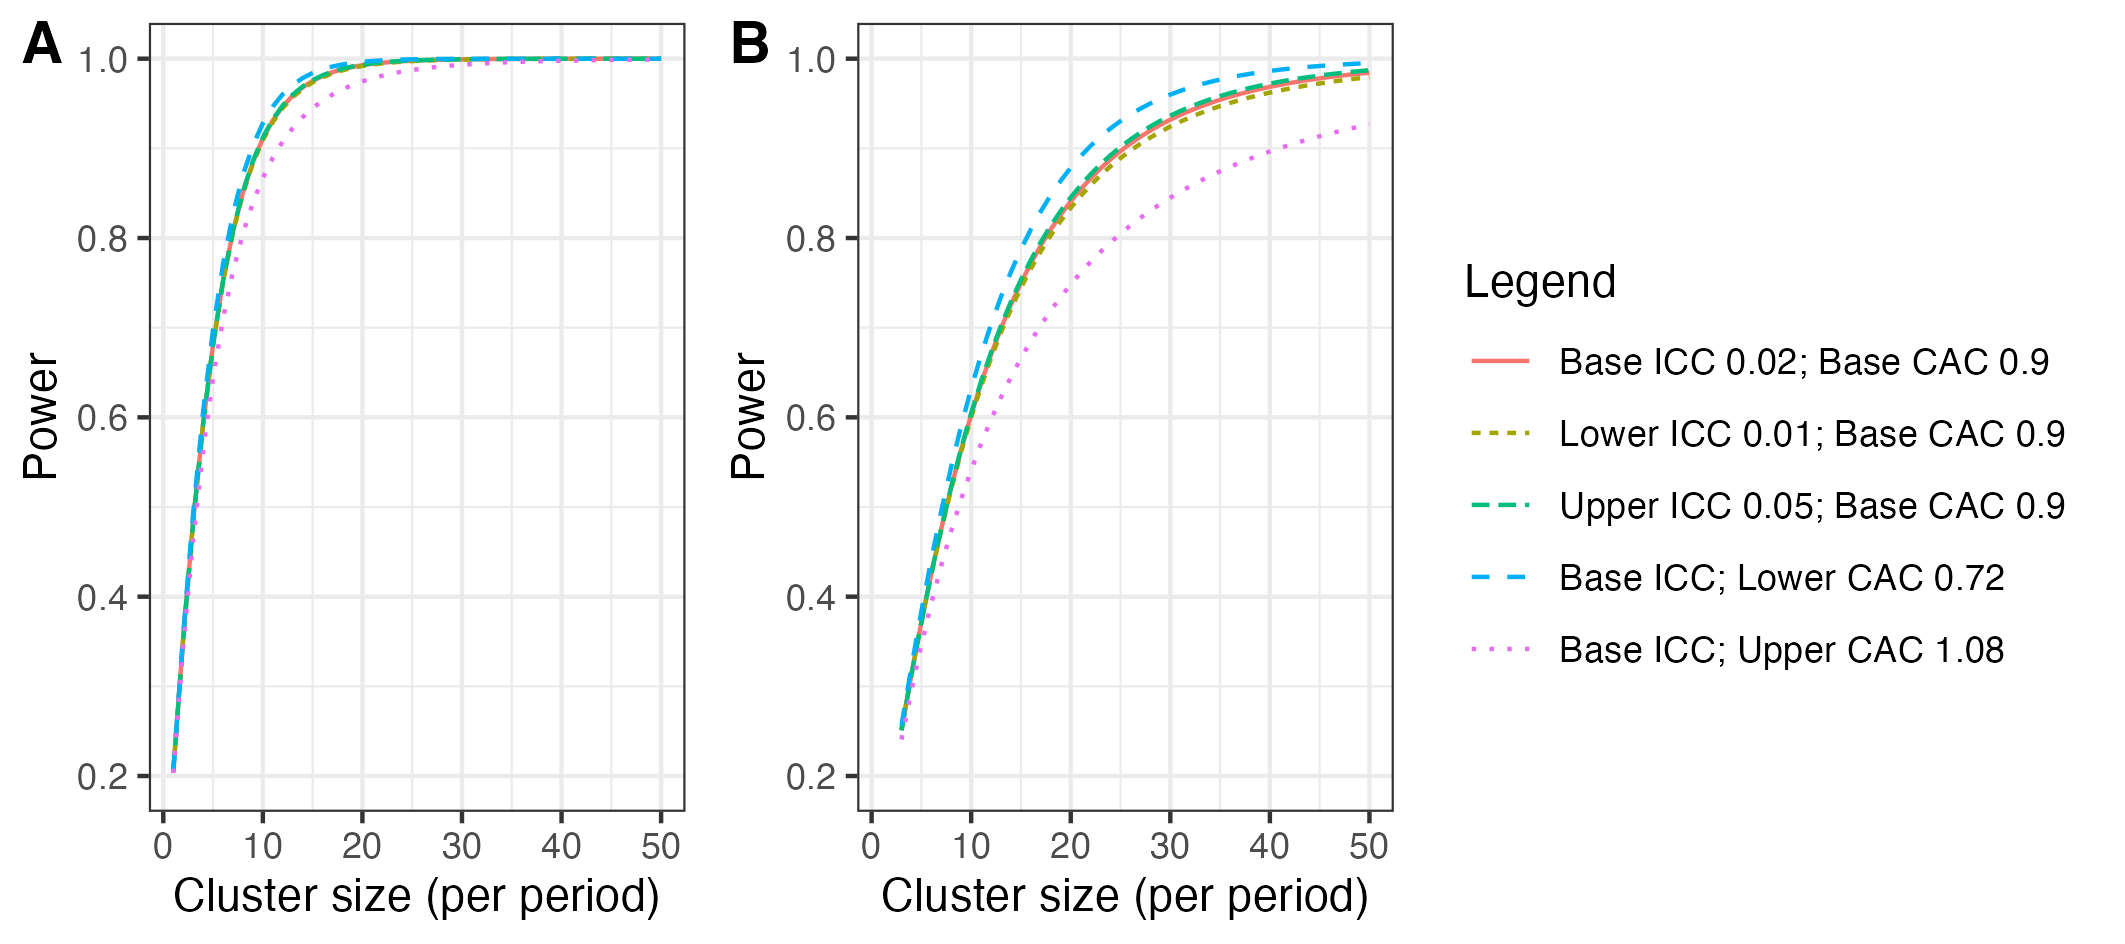
\includegraphics{./combined-power-curves.png}

}

\caption{\label{fig-power-curves}Power curves for different combinations
of cluster autocorrelations (CAC) and intra-cluster correlations (ICC).
\textbf{A)} Shows power curves assuming a reduction in the primary
outcome of in-hospital mortality within 30 days from 20\% under standard
care to 15\% after ATLS\textsuperscript{®} training. \textbf{B)} Shows
power curves assuming a reduction in the primary outcome from 10\% under
standard care to 7.5\% after ATLS\textsuperscript{®} training. Under
this scenario, we would need to increase the sample size per month to
around 30 observations to achieve 90\% powere under most combinations of
CAC and ICC.}

\end{figure}

\hypertarget{interim-analysis}{%
\subsubsection{Interim analysis}\label{interim-analysis}}

There will be one interim analyses after half of the batches have
completed the trial. The interim analyses will be assessed by the joint
Trial Steering and Data Monitoring Committee. The purposes of this
interim analysis will be to:

\begin{itemize}
\tightlist
\item
  assess the trial's feasibility and recommend stopping the trial if the
  trial is not feasible, for example if hospitals fail to adhere to the
  randomisation schedule or if there are substantial missing data in
  outcomes;
\item
  compare characteristics across intervention conditions to monitor for
  differential recruitment/ascertainment between intervention and
  control.
\end{itemize}

\hypertarget{quality-control-and-quality-assurance}{%
\subsection{Quality control and quality
assurance}\label{quality-control-and-quality-assurance}}

The George Institute for Global Health - India will ensure proper
conduct of the trial through quality control measures including on-site
training of personnel, standard operating procedures, ongoing quality
metrics assessment, review of missing data and outliers, and
round-the-clock availability of coordinating center personnel and
Principal Investigators. The trial will strictly follow ICH GCP
principles, Indian regulations, and George Institute procedures. The
trial operations staff from the George Institute India will train local
investigators, and trial site staff, before the trial, with continuous
documentation in the site master file. All documentation will be stored
securely and retained according to regulatory requirements.

\hypertarget{quality-assurance-and-oversight}{%
\subsection{Quality assurance and
oversight}\label{quality-assurance-and-oversight}}

The Trial Management Group and Trial Team, comprising key project
leaders and managers, will play a pivotal role in ensuring the highest
standards of quality assurance and effective sponsor oversight
throughout the trial. These groups will be responsible for facilitating
consistent communication, maintaining fidelity in study implementation,
and overseeing the quality of data collection.

To achieve these objectives, the groups will implement a comprehensive
communication plan and provide extensive training to site personnel. The
training will cover not only the study protocol but also practical
aspects of various systems, supplemented by both written and electronic
materials designed to educate study and clinical emergency staff.

The trial's quality assurance systems will be meticulously designed
based on a thorough risk analysis. A key component of our quality
assurance strategy will include the development and implementation of
detailed operational manuals and regular meetings. These tools and
interactions will ensure that all trial personnel will be used to uphold
the trial's quality standards.

Central to our oversight approach will be a comprehensive monitoring and
auditing plan. This plan will be tailored based on the identified risks
associated with the trial. Through these comprehensive measures, the
trial management group, in conjunction with the hospital staff, will
ensure that the trial is conducted with the utmost rigor, adhering to
the highest standards of quality assurance and effective sponsor
oversight.

\hypertarget{monitoring}{%
\subsection{Monitoring}\label{monitoring}}

We will implement a multi-tiered monitoring strategy, including
centralized data consistency checks, statistical monitoring, and
selective on-site evaluations. Key integrity measures include source
data verification, data entry validation, and regular audits. Any
protocol deviations will be thoroughly documented, with serious breaches
promptly addressed to ensure data integrity. Monitors from coordinating
centres will assist investigators in maintaining high ethical,
scientific, technical, and regulatory quality. Monitoring visits will
review protocol adherence, participant recruitment, adverse event
reporting, compliance with study procedures, and regulatory adherence.
Regular remote monitoring of the web-based database will be conducted to
ensure data integrity, using validation and consistency rules and
regular data cleaning. The Trial Team and Trial Management Group will
monitor baseline characteristics, opt-in consent rates and differential
opt-in consent rates across trial arms, follow-up rates, CRF return and
completeness rates, and safety data.

\hypertarget{deviations-serious-breaches-and-other-reporting-obligations}{%
\section{Deviations, serious breaches and other reporting
obligations}\label{deviations-serious-breaches-and-other-reporting-obligations}}

The responsible investigator shall, without delay, report to the sponsor
any serious breaches and deviations from the trial protocol, ICH-GCP and
other regulations that significantly and directly affect, or with high
likelihood could affect, the subjects' safety and integrity or the
reliability and robustness of the data generated in the trial. The
sponsor should assess the suspected serious breach and the consequences
of deviations that have occurred. Minor deviations that do not affect
subjects' integrity or safety, nor significantly affect the trial's
scientific value, are documented in the trial documentation of the
principal investigator and the sponsor and appropriate measures shall be
taken. The deviations must be recorded in the clinical trial report.

\hypertarget{audits-and-inspections}{%
\section{Audits and inspections}\label{audits-and-inspections}}

Authorized representatives for the sponsor and Competent Authorities
(CA) may carry out audits or inspections at the trial site, including
source data verification. The investigator must ensure that all source
documents are available for audits and inspections. The purpose of an
audit or inspection is to systematically and independently review all
trial-related activities and documents, to determine whether these
activities were performed, registered, analyzed and reported correctly
according to protocol, ICH- GCP and applicable regulations.

\hypertarget{ethics}{%
\section{Ethics}\label{ethics}}

\hypertarget{compliance-to-the-protocol-ich-gcp-and-regulations}{%
\subsection{Compliance to the protocol, ICH-GCP and
regulations}\label{compliance-to-the-protocol-ich-gcp-and-regulations}}

The trial will be performed in compliance with this clinical trial
protocol, the Declaration of Helsinki, ICH-GCP (Good Clinical Practice),
and current national regulations governing this clinical trial. This is
to ensure the safety and integrity of the trial subjects as well as the
quality of the data collected.

\hypertarget{ethical-review-of-the-trial}{%
\subsection{Ethical review of the
trial}\label{ethical-review-of-the-trial}}

The final protocol will be submitted for ethical review at all
participating hospitals, where possible, as well as the The George
Institute for Global Health in India and Swedish Ethical Review
Atuhortiy.

\hypertarget{procedure-for-obtaining-consent}{%
\subsection{Procedure for obtaining
consent}\label{procedure-for-obtaining-consent}}

In this trial, consent refers to data collection, as patients cannot opt
out of the intervention. This is because the intervention is implemented
at the cluster level, involving training physicians in
ATLS\textsuperscript{®}. It is unreasonable to expect these physicians
to temporarily disregard their training. Patient participants will be
included in this trial under the following modes of consent:

\begin{itemize}
\tightlist
\item
  Opt out consent for \textbf{routinely recorded data and measurement of
  adherence to ATLS\textsuperscript{®} principles}. Consent for the
  collection of routinely recorded data, either through interviews or by
  extracting information from medical records, as well as for the
  measurement of adherence to ATLS\textsuperscript{®} principles, will
  be presumed unless explicitly declined. This approach is justified
  because the trial is considered to pose minimal risk and because data
  collection will be non-invasive. Additionally, obtaining consent
  specifically for the measurement of adherence to
  ATLS\textsuperscript{®} principles could interfere with the provision
  of care and cause undue stress for the patient and their
  representatives. Patients, or their legally authorized
  representatives, will be provided with written information about the
  study upon their arrival at the hospital. The variables assumed to be
  routinely recorded are listed in Section~\ref{sec-variables}.
\item
  Opt in consent and assent for \textbf{non-routinely recorded data}.
  Informed consent for non-routinely recorded data will be actively
  sought from patient participants or their legally authorized
  representative. For participants who are between 15 and 18 years of
  age we will obtain both the assent of the participant as well as the
  consent of their guardian or legally authorized representative. The
  clinical research coordinators will approach patient participants and
  their representatives after admission. The consent and assent will be
  written for patient participants who are admitted to the hospital and
  verbal for participants who are transferred or discharged before the
  clinical research coordinators have had an opportunity to approach
  them. The verbal consent will be audio recorded.
\item
  Waiver of informed consent for patients who are unconscious or
  otherwise unable to provide consent and do not have a legally
  authorized representative. This group represents the most severly
  injured patients and they have to be included to make the trial
  representative of the entire population of trauma patients. Patients
  participants who regain consciousness will be informed about the study
  and asked for consent for collection of non-routinely recorded data.
\end{itemize}

\hypertarget{data-protection}{%
\subsection{Data protection}\label{data-protection}}

All data will be handled according to the Indian Council of Medical
Research's guidelines and standard operating procedures of the George
Institute for Global Health India on data security and protection. Trial
data will be shared via the trial electronic CRF (eCRF) throughout the
trial. The eCRF will be accessible via VPN with a two-factor
authentication and the data will be held on a secure server. All
investigators and trial site staff involved in this trial must comply
with the requirements of the ICMR Guidelines on data security and
protection. The participant information sheet provided to participants,
will inform them how:

\begin{itemize}
\tightlist
\item
  the trial data will be collected, used and disclosed;
\item
  how trial data are stored to maintain confidentiality in accordance
  with national data legislation; and
\item
  for verification of the data, representatives delegated by the
  sponsor, as well as relevant authorities, may require access to parts
  of medical records or trial records that are relevant to the trial,
  including the patient participant's medical history.
\end{itemize}

\hypertarget{insurances}{%
\section{Insurances}\label{insurances}}

The George Institute for Global Health, India is responsible for
ensuring that any insurance cover required to cover the set-up,
management and conduct of the study in India has been obtained. The
George Institute for Global Health, India is also responsible for
ensuring that India Sites have been obtained and/or will obtain
insurance prior to the opening of the study in India and shall be
maintained for the duration of the study and for an appropriate period
thereafter. This includes being responsible for ensuring that there is
appropriate insurance for the duration of the study to cover against
claims for compensation by participants arising out of their
participation in the trial in India. Compensation in case of injury or
death will be provided by the George Institute for Global Health, India
according to the regulations outlined in rules 39, 40 and 42 of the New
Drugs and Clinical Rules (2019). x

\hypertarget{substantial-changes-to-the-trial}{%
\section{Substantial changes to the
trial}\label{substantial-changes-to-the-trial}}

Substantial changes to the signed clinical trial protocol are only
possible through approved protocol amendments and by agreement between
the sponsor and the principal investigator.

\hypertarget{collection-handling-and-archiving-of-data}{%
\section{Collection, handling, and archiving of
data}\label{collection-handling-and-archiving-of-data}}

Clinical research coordinators will collect data using a paper based CRF
(see Appendix Section~\ref{sec-appendix-case-record-form}), which is
then transferred to an eCRF. All trial data in the CRF must be extracted
from and be consistent with the relevant source documents. The eCRF will
be accessible to trial coordinators, data managers, the Investigators,
Clinical Trial Monitors, Auditors, and Inspectors as required. All data
will be registered, managed, and stored in a manner that enables correct
reporting, interpretation, and verification. The complete Trial Master
File, as well as source documents, will be archived for at least 10
years after the trial is completed. Source data in the medical records
system are stored and archived in accordance with national regulations.
Metadata will be publicly accessible via a persistent DOI, and
anonymised data will be released upon project completion. A detailed
data management plan is available here
\url{https://doi.org/10.5281/zenodo.7748764}.

\hypertarget{source-data}{%
\subsection{Source data}\label{source-data}}

The source data for each variable is given in
Section~\ref{sec-variables}. Whenever medical records are the source
data, this includes imaging and lab reports. Whenever an interview is
given as the source, the CRF will constitute the source data, as this is
where the responses to questions will be recorded. The local
investigator must keep source documents for each patient participant in
the trial. A document describing what has been classified as source data
in the trial (source data reference document) will be included in the
Investigator Site File (ISF). The investigator must ensure that all
source documents are accessible for monitoring and other quality control
activities. Source data is further defined before trial start at each
individual site and can, in cases where source data is not registered in
another document, consist of the CRF. This should be decided in
consultation with the monitor and clearly stated in the source data
reference document. Access to trial-related documentation, such as
patient participants' medical records, CRFs, other source data and other
trial documentation will be provided for monitoring and auditing
purposes. Access will also be granted in the context of regulatory
inspections.

\hypertarget{sec-variables}{%
\subsection{Variables}\label{sec-variables}}

\hypertarget{screening-v10011024}{%
\subsubsection{Screening v10011024}\label{screening-v10011024}}

\begin{itemize}
\item
  \textbf{Screening ID}
\item
  \textbf{1. Date of screening}
\item
  \textbf{2. Date of data entry}
\item
  \textbf{1. Is the patient at least 15 years old?} Source: Medical
  record or interview

  \begin{enumerate}
  \def\labelenumi{\arabic{enumi}.}
  \tightlist
  \item
    Yes
  \item
    No
  \end{enumerate}
\item
  \textbf{2. Did the patient present with a history of trauma defined as
  having any of the reasons listed in the International Classification
  of Diseases chapter XX as the reason for presenting? Please see
  https://icd.who.int/browse10/2019/en\#/XX for a complete list of
  ICD-10 codes} Source: Medical record or interview

  \begin{enumerate}
  \def\labelenumi{\arabic{enumi}.}
  \tightlist
  \item
    Yes
  \item
    No
  \end{enumerate}
\item
  \textbf{3. Did the trauma occur less than 48 hours before arrival to
  the hospital?} Source: Medical record or interview

  \begin{enumerate}
  \def\labelenumi{\arabic{enumi}.}
  \tightlist
  \item
    Yes
  \item
    No
  \end{enumerate}
\item
  \textbf{4. Was the patient admitted?} Source: Medical record

  \begin{enumerate}
  \def\labelenumi{\arabic{enumi}.}
  \tightlist
  \item
    Yes
  \item
    No
  \end{enumerate}
\item
  \textbf{5. Did the patient die after arrival but before admission?}
  Source: Medical record

  \begin{enumerate}
  \def\labelenumi{\arabic{enumi}.}
  \tightlist
  \item
    Yes
  \item
    No
  \end{enumerate}
\item
  \textbf{6. Was the patient transferred to another hospital for
  admission?} Source: Medical record

  \begin{enumerate}
  \def\labelenumi{\arabic{enumi}.}
  \tightlist
  \item
    Yes
  \item
    No
  \end{enumerate}
\item
  \textbf{1. Did the patient present with isolated limb injury?} Source:
  Medical record

  \begin{enumerate}
  \def\labelenumi{\arabic{enumi}.}
  \tightlist
  \item
    Yes
  \item
    No
  \end{enumerate}
\item
  \textbf{2. Was the patient directly admitted to a ward without being
  seen by a physician in the emergency department?} Source: Medical
  record

  \begin{enumerate}
  \def\labelenumi{\arabic{enumi}.}
  \tightlist
  \item
    Yes
  \item
    No
  \end{enumerate}
\end{itemize}

\hypertarget{consent-v10011024}{%
\subsubsection{Consent v10011024}\label{consent-v10011024}}

\begin{itemize}
\item
  \textbf{1. Is this patient included under the waiver of informed
  consent because the patient is unconscious or otherwise unable to
  provide consent and do not have a legally acceptable representative?}

  \begin{enumerate}
  \def\labelenumi{\arabic{enumi}.}
  \tightlist
  \item
    Yes
  \item
    No
  \end{enumerate}
\item
  \textbf{1. Did the participant/ or legally acceptable representative
  (LAR) provided consent for collection of non-routinely recorded data}

  \begin{enumerate}
  \def\labelenumi{\arabic{enumi}.}
  \tightlist
  \item
    Yes
  \item
    No
  \end{enumerate}
\item
  \textbf{2. Who gave consent for collection of non-routinely recorded
  data?}

  \begin{enumerate}
  \def\labelenumi{\arabic{enumi}.}
  \tightlist
  \item
    Patient participant
  \item
    Legally acceptable representative
  \end{enumerate}
\item
  \textbf{3. Relation of LAR with the Participant}
\item
  \textbf{4. Why was Legally acceptable representative (LAR) approached
  for consent for collection of non-routinely recorded data?}

  \begin{enumerate}
  \def\labelenumi{\arabic{enumi}.}
  \tightlist
  \item
    The participant is incapacitated because of the trauma
  \item
    The participant is younger than 18 years
  \end{enumerate}
\item
  \textbf{5. Date when participant or legally acceptable representative
  (LAR) gave consent for collection of non-routinely recorded data?}
\item
  \textbf{6. How did the participant or legally acceptable
  representative (LAR) consent for collection of non-routinely recorded
  data?}

  \begin{enumerate}
  \def\labelenumi{\arabic{enumi}.}
  \tightlist
  \item
    In writing
  \item
    Verbally
  \end{enumerate}
\item
  \textbf{7. Date when the participant was reconsented?}
\item
  \textbf{1. Did the minor give assent for collection of non-routinely
  recorded data?}

  \begin{enumerate}
  \def\labelenumi{\arabic{enumi}.}
  \tightlist
  \item
    Yes
  \item
    No
  \end{enumerate}
\item
  \textbf{2. Date when the minor gave assent for collection of
  non-routinely recorded data.}
\item
  \textbf{3. In case the minor refused to participate, date when minor
  refused}
\item
  \textbf{1. Is the participant or LAR wants to opt out from study?}

  \begin{enumerate}
  \def\labelenumi{\arabic{enumi}.}
  \tightlist
  \item
    Yes
  \item
    No
  \end{enumerate}
\item
  \textbf{2. Who opted-out of the routinely recorded data
  (in-hospital)?}

  \begin{enumerate}
  \def\labelenumi{\arabic{enumi}.}
  \tightlist
  \item
    Patient participant
  \item
    Legally acceptable representative (LAR)
  \end{enumerate}
\item
  \textbf{3. Date when participant or legally acceptable representative
  (LAR) opted-out.}
\item
  \textbf{4. Did the participant or legally acceptable representative
  (LAR) suggested to delete all the previously recorded data?}

  \begin{enumerate}
  \def\labelenumi{\arabic{enumi}.}
  \tightlist
  \item
    Yes
  \item
    No
  \end{enumerate}
\end{itemize}

\hypertarget{consent-withdrawn-v10011024}{%
\subsubsection{Consent withdrawn
v10011024}\label{consent-withdrawn-v10011024}}

\begin{itemize}
\item
  \textbf{1. Does the participant or legally acceptable representative
  (LAR) want to withdraw the consent?}

  \begin{enumerate}
  \def\labelenumi{\arabic{enumi}.}
  \tightlist
  \item
    Yes
  \item
    No
  \end{enumerate}
\item
  \textbf{2. Date of consent withdrawal for follow-up data collection.}
\item
  \textbf{3. Procedure(s) for which consent has been withdrawn}

  \begin{enumerate}
  \def\labelenumi{\arabic{enumi}.}
  \tightlist
  \item
    Data collection prior to withdrawal
  \item
    All data collection after withdrawal
  \item
    Both
  \end{enumerate}
\end{itemize}

\hypertarget{baseline-v10011024}{%
\subsubsection{Baseline v10011024}\label{baseline-v10011024}}

\begin{itemize}
\item
  \textbf{1. Age in years} Source: Medical record of interview
\item
  \textbf{2. Sex} Source: Medical record of interview

  \begin{enumerate}
  \def\labelenumi{\arabic{enumi}.}
  \tightlist
  \item
    Female
  \item
    Male
  \item
    Other
  \item
    Not known
  \end{enumerate}
\item
  \textbf{3. Current marital status} Requires opt-in consent, not
  routinely recorded. Source: Interview

  \begin{enumerate}
  \def\labelenumi{\arabic{enumi}.}
  \tightlist
  \item
    Never married
  \item
    Currently married
  \item
    Separated
  \item
    Divorced
  \item
    Widowed
  \item
    Cohabiting
  \item
    Not known
  \end{enumerate}
\item
  \textbf{4. Education level} Requires opt-in consent, not routinely
  recorded. Source: Interview

  \begin{enumerate}
  \def\labelenumi{\arabic{enumi}.}
  \tightlist
  \item
    Not attended school
  \item
    Primary school
  \item
    Secondary school
  \item
    Higher secondary school
  \item
    Graduate
  \item
    Post graduate and above
  \item
    Other
  \item
    Not known
  \end{enumerate}
\item
  \textbf{5. If other, please specify} Requires opt-in consent, not
  routinely recorded. Source: Interview
\item
  \textbf{6. Main work status} Requires opt-in consent, not routinely
  recorded. Source: Interview

  \begin{enumerate}
  \def\labelenumi{\arabic{enumi}.}
  \tightlist
  \item
    Paid work, such as daily wage earner, teacher, factory worker and
    government employee
  \item
    Self-employed, such as own your business or farming
  \item
    Non-paid work, such as volunteer or charity
  \item
    Student
  \item
    Keeping house/homemaker
  \item
    Retired
  \item
    Unemployed (health reasons)
  \item
    Unemployed (other reasons)
  \item
    Other
  \item
    No income
  \item
    Not known
  \end{enumerate}
\item
  \textbf{7. If other, please specify} Requires opt-in consent, not
  routinely recorded. Source: Interview
\item
  \textbf{8. Income level in INR per month} Requires opt-in consent, not
  routinely recorded. Source: Interview

  \begin{enumerate}
  \def\labelenumi{\arabic{enumi}.}
  \tightlist
  \item
    Below 10,000
  \item
    10,001-20,000
  \item
    20,001-30,000
  \item
    30,001-50,000
  \item
    50,001-80,000
  \item
    80,001-1,00,000
  \item
    Above 1,00,000
  \item
    Not known
  \end{enumerate}
\item
  \textbf{9. Mechanism of injury} Coded using ICD 10. Source: Medical
  record
\item
  \textbf{10. Clinical Frailty Scale} Source: Medical record or treating
  physician

  \begin{enumerate}
  \def\labelenumi{\arabic{enumi}.}
  \item
    \begin{enumerate}
    \def\labelenumii{\arabic{enumii}.}
    \tightlist
    \item
      Very fit
    \end{enumerate}
  \item
    \begin{enumerate}
    \def\labelenumii{\arabic{enumii}.}
    \setcounter{enumii}{1}
    \tightlist
    \item
      Fit
    \end{enumerate}
  \item
    \begin{enumerate}
    \def\labelenumii{\arabic{enumii}.}
    \setcounter{enumii}{2}
    \tightlist
    \item
      Managing well
    \end{enumerate}
  \item
    \begin{enumerate}
    \def\labelenumii{\arabic{enumii}.}
    \setcounter{enumii}{3}
    \tightlist
    \item
      Living with very mild frailty
    \end{enumerate}
  \item
    \begin{enumerate}
    \def\labelenumii{\arabic{enumii}.}
    \setcounter{enumii}{4}
    \tightlist
    \item
      Living with mild frailty
    \end{enumerate}
  \item
    \begin{enumerate}
    \def\labelenumii{\arabic{enumii}.}
    \setcounter{enumii}{5}
    \tightlist
    \item
      Living with moderate frailty
    \end{enumerate}
  \item
    \begin{enumerate}
    \def\labelenumii{\arabic{enumii}.}
    \setcounter{enumii}{6}
    \tightlist
    \item
      Living with severe frailty
    \end{enumerate}
  \item
    \begin{enumerate}
    \def\labelenumii{\arabic{enumii}.}
    \setcounter{enumii}{7}
    \tightlist
    \item
      Living with very severe frailty
    \end{enumerate}
  \item
    \begin{enumerate}
    \def\labelenumii{\arabic{enumii}.}
    \setcounter{enumii}{8}
    \tightlist
    \item
      Terminally ill
    \end{enumerate}
  \item
    Not known
  \end{enumerate}
\item
  \textbf{11. Comorbidities (Charlson Comorbidity Index)} Source:
  Medical record, treating physician or interview

  \begin{enumerate}
  \def\labelenumi{\arabic{enumi}.}
  \tightlist
  \item
    Myocardial infarction
  \item
    Congestive heart failure
  \item
    Peripheral vascular disease
  \item
    Cerebrovascular disease
  \item
    Dementia
  \item
    Chronic pulmonary disease
  \item
    Rheumatologic disease
  \item
    Peptic ulcer disease
  \item
    Liver disease
  \item
    Diabetes
  \item
    Hemiplegia or paraplegia
  \item
    Renal disease
  \item
    Malignancy
  \item
    Leukemia
  \item
    Lymphoma
  \item
    AIDS
  \item
    Not known
  \item
    None
  \end{enumerate}
\item
  \textbf{12. Severity of liver disease} Source: Medical record,
  treating physician or interview

  \begin{enumerate}
  \def\labelenumi{\arabic{enumi}.}
  \tightlist
  \item
    Mild
  \item
    Moderate or severe
  \item
    Not known
  \end{enumerate}
\item
  \textbf{13. Severity of diabetes} Source: Medical record, treating
  physician or interview

  \begin{enumerate}
  \def\labelenumi{\arabic{enumi}.}
  \tightlist
  \item
    Controlled
  \item
    Uncontrolled
  \item
    Not known
  \end{enumerate}
\item
  \textbf{14. Severity of malignancy} Source: Medical record, treating
  physician or interview

  \begin{enumerate}
  \def\labelenumi{\arabic{enumi}.}
  \tightlist
  \item
    Localized
  \item
    Metastatic tumor
  \item
    Not known
  \end{enumerate}
\end{itemize}

\hypertarget{prehospital-v10011024}{%
\subsubsection{Prehospital v10011024}\label{prehospital-v10011024}}

\begin{itemize}
\item
  \textbf{1. Date and time of injury} Source: Medical record of
  interview
\item
  \textbf{2. Mode of transport to the participating hospital} Source:
  Medical record of interview

  \begin{enumerate}
  \def\labelenumi{\arabic{enumi}.}
  \tightlist
  \item
    Ambulance
  \item
    Police
  \item
    Private vehicle
  \item
    Walking
  \item
    Others
  \item
    Not known
  \end{enumerate}
\item
  \textbf{3. If other, please specify} Source: Medical record of
  interview
\item
  \textbf{4. Referred or transferred to the participating hospital from
  another hospital} Source: Medical record of interview

  \begin{enumerate}
  \def\labelenumi{\arabic{enumi}.}
  \tightlist
  \item
    Yes
  \item
    No
  \item
    Not known
  \end{enumerate}
\end{itemize}

\hypertarget{atls-adherence-v11221024}{%
\subsubsection{ATLS adherence
v11221024}\label{atls-adherence-v11221024}}

\begin{itemize}
\item
  \textbf{1. Airway patency checked} Source: Observation

  \begin{enumerate}
  \def\labelenumi{\arabic{enumi}.}
  \tightlist
  \item
    Yes
  \item
    No
  \end{enumerate}
\item
  \textbf{1. Chest wall palpated} Source: Observation

  \begin{enumerate}
  \def\labelenumi{\arabic{enumi}.}
  \tightlist
  \item
    Yes
  \item
    No
  \end{enumerate}
\item
  \textbf{2. Breath sounds checked} Source: Observation

  \begin{enumerate}
  \def\labelenumi{\arabic{enumi}.}
  \tightlist
  \item
    Yes
  \item
    No
  \end{enumerate}
\item
  \textbf{3. Respiratory rate measured} Source: Observation

  \begin{enumerate}
  \def\labelenumi{\arabic{enumi}.}
  \tightlist
  \item
    Yes
  \item
    No
  \end{enumerate}
\item
  \textbf{4. Saturation (SpO2) measured} Source: Observation

  \begin{enumerate}
  \def\labelenumi{\arabic{enumi}.}
  \tightlist
  \item
    Yes
  \item
    No
  \end{enumerate}
\item
  \textbf{1. Heart rate measured} Source: Observation

  \begin{enumerate}
  \def\labelenumi{\arabic{enumi}.}
  \tightlist
  \item
    Yes
  \item
    No
  \end{enumerate}
\item
  \textbf{2. Blood pressure measured} Source: Observation

  \begin{enumerate}
  \def\labelenumi{\arabic{enumi}.}
  \tightlist
  \item
    Yes
  \item
    No
  \end{enumerate}
\item
  \textbf{3. Abdomen palpated} Source: Observation

  \begin{enumerate}
  \def\labelenumi{\arabic{enumi}.}
  \tightlist
  \item
    Yes
  \item
    No
  \end{enumerate}
\item
  \textbf{4. Thighs palpated} Source: Observation

  \begin{enumerate}
  \def\labelenumi{\arabic{enumi}.}
  \tightlist
  \item
    Yes
  \item
    No
  \end{enumerate}
\item
  \textbf{5. IV access obtained} Source: Observation

  \begin{enumerate}
  \def\labelenumi{\arabic{enumi}.}
  \tightlist
  \item
    Yes
  \item
    No
  \end{enumerate}
\item
  \textbf{1. GCS checked} Source: Observation

  \begin{enumerate}
  \def\labelenumi{\arabic{enumi}.}
  \tightlist
  \item
    Yes
  \item
    No
  \end{enumerate}
\item
  \textbf{2. Pupils checked} Source: Observation

  \begin{enumerate}
  \def\labelenumi{\arabic{enumi}.}
  \tightlist
  \item
    Yes
  \item
    No
  \end{enumerate}
\item
  \textbf{1. Patients exposed for assessment}

  \begin{enumerate}
  \def\labelenumi{\arabic{enumi}.}
  \tightlist
  \item
    Yes
  \item
    No
  \end{enumerate}
\item
  \textbf{2. Temperature measured} Source: Observation

  \begin{enumerate}
  \def\labelenumi{\arabic{enumi}.}
  \tightlist
  \item
    Yes
  \item
    No
  \end{enumerate}
\item
  \textbf{1. Which airway interventions were performed?} Source:
  Observation

  \begin{enumerate}
  \def\labelenumi{\arabic{enumi}.}
  \tightlist
  \item
    None
  \item
    Manual airway procedure such as chin lift or jaw thrust
  \item
    Nasopharyngeal or Oropharyngeal airway inserted
  \item
    Supraglottic airway device
  \item
    Tracheal intubation
  \item
    Surgical airway
  \item
    Other
  \item
    Not known
  \end{enumerate}
\item
  \textbf{2. If other airway Interventions given, specify}
\item
  \textbf{3. Were airway interventions performed while minimising
  c-spine movement?} Source: Observation

  \begin{enumerate}
  \def\labelenumi{\arabic{enumi}.}
  \tightlist
  \item
    Yes
  \item
    No
  \item
    Not known
  \end{enumerate}
\item
  \textbf{1. Which breathing interventions were performed?} Source:
  Observation

  \begin{enumerate}
  \def\labelenumi{\arabic{enumi}.}
  \tightlist
  \item
    None
  \item
    Oxygen applied
  \item
    Intracostal drain placement
  \item
    Other
  \item
    Not done
  \item
    Not known
  \end{enumerate}
\item
  \textbf{2. If other breathing Interventions done, specify}
\item
  \textbf{1. Which circulation interventions and adjuncts were
  performed?} Source: Observation

  \begin{enumerate}
  \def\labelenumi{\arabic{enumi}.}
  \tightlist
  \item
    None
  \item
    Control of external bleeding
  \item
    Fluid bolus
  \item
    Blood transfusion
  \item
    eFast
  \item
    Pelvic binder applied
  \item
    Reduction of highly displaced fracture
  \item
    Other
  \item
    Not known
  \end{enumerate}
\item
  \textbf{2. If other circulation Interventions done, specify}
\item
  \textbf{1. Which disability intervention was performed?} Source:
  Observation

  \begin{enumerate}
  \def\labelenumi{\arabic{enumi}.}
  \tightlist
  \item
    None
  \item
    Placement of definitive airway if the patient had a GCS of 8 or less
  \item
    Log Rolling
  \item
    Spine board during transportation
  \item
    Other
  \item
    Not known
  \end{enumerate}
\item
  \textbf{2. If other disability interventions done, specify}
\item
  \textbf{1. Which exposure intervention was performed?} Source:
  Observation

  \begin{enumerate}
  \def\labelenumi{\arabic{enumi}.}
  \tightlist
  \item
    None
  \item
    Covered with warmer or blanket
  \item
    Warm fluids administered
  \item
    Other
  \item
    Not known
  \end{enumerate}
\item
  \textbf{2. If other exposure interventions done, specify}
\end{itemize}

\hypertarget{emergency-department-v10011024}{%
\subsubsection{Emergency department
v10011024}\label{emergency-department-v10011024}}

\begin{itemize}
\item
  \textbf{1. Date and time of arrival to the emergency department at the
  participating hospital} Source: Medical record of interview
\item
  \textbf{2. First recorded systolic blood pressure (mmHg)} Source:
  Medical record
\item
  \textbf{3. First recorded diastolic blood pressure (mmHg)} Source:
  Medical record
\item
  \textbf{4. First recorded heart rate (beats per minute)} Source:
  Medical record
\item
  \textbf{5. First recorded respiratory rate (breaths per minute)}
  Source: Medical record
\item
  \textbf{6. First recorded Glasgow Coma Scale} Source: Medical record
\item
  \textbf{7. First recorded body temperature (°C)} Source: Medical
  record
\item
  \textbf{8. First recorded oxygen saturation (\%)} Source: Medical
  record
\item
  \textbf{9. Emergency department disposition} Source: Medical record

  \begin{enumerate}
  \def\labelenumi{\arabic{enumi}.}
  \tightlist
  \item
    Admitted
  \item
    Referred or transferred for admission
  \item
    Dead
  \item
    Others
  \item
    Not known
  \end{enumerate}
\item
  \textbf{10. If other, please specify} Source: Medical record
\item
  \textbf{11. Date and time of referral or transfer for admission}
  Source: Medical record
\end{itemize}

\hypertarget{hospital-v10011024}{%
\subsubsection{Hospital v10011024}\label{hospital-v10011024}}

\begin{itemize}
\item
  \textbf{1. Date of admission to the participating hospital} Source:
  Medical record
\item
  \textbf{1.1 Time of admission to the participating hospital} Source:
  Medical record
\item
  \textbf{2. Type of admitting ward} Source: Medical record

  \begin{enumerate}
  \def\labelenumi{\arabic{enumi}.}
  \tightlist
  \item
    General surgery
  \item
    Orthopaedics
  \item
    Neurosurgery
  \item
    Intensive care unit
  \item
    High dependency unit
  \item
    Medicine
  \item
    Trauma ward
  \item
    Not known
  \end{enumerate}
\item
  \textbf{3. Ward name or number} Source: Medical record
\item
  \textbf{4. Admitted to intensive care unit during admission} Source:
  Medical record

  \begin{enumerate}
  \def\labelenumi{\arabic{enumi}.}
  \tightlist
  \item
    Yes
  \item
    No
  \item
    Not known
  \end{enumerate}
\item
  \textbf{5. Date of first intensive care unit admission} Source:
  Medical record
\item
  \textbf{5.1 Time of first intensive care unit admission} Source:
  Medical record
\item
  \textbf{6. Date of first intensive care unit discharge} Source:
  Medical record
\item
  \textbf{6.1 Time of first intensive care unit discharge} Source:
  Medical record
\item
  \textbf{7. Hospital disposition} Source: Medical record

  \begin{enumerate}
  \def\labelenumi{\arabic{enumi}.}
  \tightlist
  \item
    Alive
  \item
    Dead
  \item
    Transferred for admission
  \item
    Not known
  \end{enumerate}
\item
  \textbf{8. Was the patient transferred to another hospital for
  admission?} Source: Medical record

  \begin{enumerate}
  \def\labelenumi{\arabic{enumi}.}
  \tightlist
  \item
    Yes
  \item
    No
  \item
    Not known
  \end{enumerate}
\item
  \textbf{9. Date of discharge or transfer from participating hospital}
  Source: Medical record
\item
  \textbf{9.1 Time of discharge or transfer from participating hospital}
  Source: Medical record
\end{itemize}

\hypertarget{surgery-v10011024}{%
\subsubsection{Surgery v10011024}\label{surgery-v10011024}}

\begin{itemize}
\item
  \textbf{1. Date of surgical procedure} A surgical procedure is defined
  as any procedure performed in the operating room, interventional
  dropdownlogy suite, or at the bedside, requiring general or regional
  anesthesia. Source: Medical record
\item
  \textbf{1. Time of surgical procedure} A surgical procedure is defined
  as any procedure performed in the operating room, interventional
  dropdownlogy suite, or at the bedside, requiring general or regional
  anesthesia. Source: Medical record
\item
  \textbf{2. Preoperative ASA score} Source: Medical record or treating
  physician

  \begin{enumerate}
  \def\labelenumi{\arabic{enumi}.}
  \item
    \begin{enumerate}
    \def\labelenumii{\arabic{enumii}.}
    \tightlist
    \item
      A normal healthy patient
    \end{enumerate}
  \item
    \begin{enumerate}
    \def\labelenumii{\arabic{enumii}.}
    \setcounter{enumii}{1}
    \tightlist
    \item
      A patient with mild systemic disease
    \end{enumerate}
  \item
    \begin{enumerate}
    \def\labelenumii{\arabic{enumii}.}
    \setcounter{enumii}{2}
    \tightlist
    \item
      A patient with severe systemic disease
    \end{enumerate}
  \item
    \begin{enumerate}
    \def\labelenumii{\arabic{enumii}.}
    \setcounter{enumii}{3}
    \tightlist
    \item
      A patient with severe systemic disease that is a constant threat
      to life
    \end{enumerate}
  \item
    \begin{enumerate}
    \def\labelenumii{\arabic{enumii}.}
    \setcounter{enumii}{4}
    \tightlist
    \item
      A moribund patient who is not expected to survive without the
      operation
    \end{enumerate}
  \item
    \begin{enumerate}
    \def\labelenumii{\arabic{enumii}.}
    \setcounter{enumii}{5}
    \tightlist
    \item
      A declared brain-dead patient whose organs are being removed for
      donor purposes
    \end{enumerate}
  \item
    \begin{enumerate}
    \def\labelenumii{\arabic{enumii}.}
    \setcounter{enumii}{998}
    \tightlist
    \item
      Not known
    \end{enumerate}
  \end{enumerate}
\item
  \textbf{3. Description of procedure} Source: Medical record
\item
  \textbf{4. Procedure coded according to SNOMED CT} Source: Medical
  record
\end{itemize}

\hypertarget{imaging-v10011024}{%
\subsubsection{Imaging v10011024}\label{imaging-v10011024}}

\begin{itemize}
\item
  \textbf{1. Date and time of imaging} Source: Medical record
\item
  \textbf{1.1 Time of imaging} Source: Medical record
\item
  \textbf{2. Type of imaging} Source: Medical record

  \begin{enumerate}
  \def\labelenumi{\arabic{enumi}.}
  \tightlist
  \item
    Ultrasound
  \item
    X-ray
  \item
    Computed Tomography (CT)
  \item
    Magnetic Resonance Imaging (MRI)
  \end{enumerate}
\end{itemize}

\hypertarget{transfusion-v10011024}{%
\subsubsection{Transfusion v10011024}\label{transfusion-v10011024}}

\begin{itemize}
\item
  \textbf{1. Date of transfusion} Source: Medical record
\item
  \textbf{1.1 Time of transfusion} Source: Medical record
\item
  \textbf{2. Type of blood product} Source: Medical record

  \begin{enumerate}
  \def\labelenumi{\arabic{enumi}.}
  \tightlist
  \item
    Packed red blood cells
  \item
    Platelets
  \item
    Fresh frozen plasma
  \item
    Whole blood
  \item
    Other
  \end{enumerate}
\item
  \textbf{2.1 Other specify}
\item
  \textbf{3. Number of units transfused} Source: Medical record
\end{itemize}

\hypertarget{injury-v10011024}{%
\subsubsection{Injury v10011024}\label{injury-v10011024}}

\begin{itemize}
\item
  \textbf{1. Injury description} Source: Medical record
\item
  \textbf{2. ICD 10 code} Coded using ICD 10. Source: Medical record
\item
  \textbf{3. Injury source data} Source: Medical record

  \begin{enumerate}
  \def\labelenumi{\arabic{enumi}.}
  \tightlist
  \item
    Medical record
  \item
    X-ray report
  \item
    CT-report
  \item
    Surgical notes
  \end{enumerate}
\item
  \textbf{4. Injury time}
\end{itemize}

\hypertarget{individual-mortality-status-v10011024}{%
\subsubsection{Individual mortality status
v10011024}\label{individual-mortality-status-v10011024}}

\begin{itemize}
\tightlist
\item
  \textbf{1. Is the patient dead?} Source: Medical record or interview

  \begin{enumerate}
  \def\labelenumi{\arabic{enumi}.}
  \tightlist
  \item
    Yes
  \item
    No
  \end{enumerate}
\item
  \textbf{2. Date and time of death} Source: Medical record or interview
\end{itemize}

\hypertarget{quality-of-life-eq5d5l}{%
\subsubsection{Quality of life (EQ5D5L)}\label{quality-of-life-eq5d5l}}

\begin{itemize}
\item
  \textbf{Date of filling this form}
\item
  \textbf{First, I would like to ask you about MOBILITY. Would you say
  that:} Requires opt-in consent, not routinely recorded. Source:
  Interview

  \begin{enumerate}
  \def\labelenumi{\arabic{enumi}.}
  \tightlist
  \item
    You have no problems in walking about?
  \item
    You have slight problems in walking about?
  \item
    You have moderate problems in walking about?
  \item
    You have severe problems in walking about?
  \item
    You are unable to walk about?
  \end{enumerate}
\item
  \textbf{Next, I would like to ask you about SELF-CARE. Would you say
  that:} Requires opt-in consent, not routinely recorded. Source:
  Interview

  \begin{enumerate}
  \def\labelenumi{\arabic{enumi}.}
  \tightlist
  \item
    You have no problems washing or dressing yourself?
  \item
    You have slight problems washing or dressing yourself?
  \item
    You have moderate problems washing or dressing yourself?
  \item
    You have severe problems washing or dressing yourself?
  \item
    You are unable to wash or dress yourself?
  \end{enumerate}
\item
  \textbf{Next, I would like to ask you about USUAL ACTIVITIES, for
  example, work, study, housework, family or leisure activities. Would
  you say that:} Requires opt-in consent, not routinely recorded.
  Source: Interview

  \begin{enumerate}
  \def\labelenumi{\arabic{enumi}.}
  \tightlist
  \item
    You have no problems doing your usual activities?
  \item
    You have slight problems doing your usual activities?
  \item
    You have moderate problems doing your usual activities?
  \item
    You have severe problems doing your usual activities?
  \item
    You are unable to do your usual activities?
  \end{enumerate}
\item
  \textbf{Next, I would like to ask you about PAIN OR DISCOMFORT. Would
  you say that:} Requires opt-in consent, not routinely recorded.
  Source: Interview

  \begin{enumerate}
  \def\labelenumi{\arabic{enumi}.}
  \tightlist
  \item
    You have no pain or discomfort?
  \item
    You have slight pain or discomfort?
  \item
    You have moderate pain or discomfort?
  \item
    You have severe pain or discomfort?
  \item
    You have extreme pain or discomfort?
  \end{enumerate}
\item
  \textbf{Finally, I would like to ask you about ANXIETY OR DEPRESSION.
  Would you say that:} Requires opt-in consent, not routinely recorded.
  Source: Interview

  \begin{enumerate}
  \def\labelenumi{\arabic{enumi}.}
  \tightlist
  \item
    You are not anxious or depressed?
  \item
    You are slightly anxious or depressed?
  \item
    You are moderately anxious or depressed?
  \item
    You are severely anxious or depressed?
  \item
    You are extremely anxious or depressed?
  \end{enumerate}
\item
  \textbf{~ I would now like you to tell me the point on this line where
  you would put your health TODAY.(Note to interviewer: mark the line at
  the point indicating the respondent's health today.) ~} Requires
  opt-in consent, not routinely recorded. Source: Interview
\end{itemize}

\hypertarget{disability-whodas-2.0}{%
\subsubsection{Disability (WHODAS 2.0)}\label{disability-whodas-2.0}}

\begin{itemize}
\item
  \textbf{Date of form filling}
\item
  \textbf{1. Who are you interviewing?} Requires opt-in consent, not
  routinely recorded. Source: Interview

  \begin{enumerate}
  \def\labelenumi{\arabic{enumi}.}
  \tightlist
  \item
    Patient participant
  \item
    Patient representative
  \end{enumerate}
\item
  \textbf{2. What is the relationship between the representative and the
  participant?} Requires opt-in consent, not routinely recorded. Source:
  Interview

  \begin{enumerate}
  \def\labelenumi{\arabic{enumi}.}
  \tightlist
  \item
    Husband or wife
  \item
    Parent
  \item
    Son or daughter
  \item
    Brother or sister
  \item
    Other relative
  \item
    Friend
  \item
    Professional carer
  \item
    Other (specify)
  \end{enumerate}
\item
  \textbf{3. If other, please specify}
\item
  \textbf{1. Standing for long periods such as 30 minutes?} Requires
  opt-in consent, not routinely recorded. Source: Interview

  \begin{enumerate}
  \def\labelenumi{\arabic{enumi}.}
  \tightlist
  \item
    None
  \item
    Mild
  \item
    Moderate
  \item
    Severe
  \item
    Extreme or cannot do
  \item
    None
  \item
    Mild
  \item
    Moderate
  \item
    Severe
  \item
    Extreme or cannot do
  \end{enumerate}
\item
  \textbf{1. Standing for long periods such as 30 minutes?} Requires
  opt-in consent, not routinely recorded. Source: Interview

  \begin{enumerate}
  \def\labelenumi{\arabic{enumi}.}
  \tightlist
  \item
    None
  \item
    Mild
  \item
    Moderate
  \item
    Severe
  \item
    Extreme or cannot do
  \item
    None
  \item
    Mild
  \item
    Moderate
  \item
    Severe
  \item
    Extreme or cannot do
  \end{enumerate}
\item
  \textbf{2. Taking care of your household responsibilities?} Requires
  opt-in consent, not routinely recorded. Source: Interview

  \begin{enumerate}
  \def\labelenumi{\arabic{enumi}.}
  \tightlist
  \item
    None
  \item
    Mild
  \item
    Moderate
  \item
    Severe
  \item
    Extreme or cannot do
  \end{enumerate}
\item
  \textbf{3. Learning a new task, for example, learning how to get to a
  new place?} Requires opt-in consent, not routinely recorded. Source:
  Interview

  \begin{enumerate}
  \def\labelenumi{\arabic{enumi}.}
  \tightlist
  \item
    None
  \item
    Mild
  \item
    Moderate
  \item
    Severe
  \item
    Extreme or cannot do
  \item
    None
  \item
    Mild
  \item
    Moderate
  \item
    Severe
  \item
    Extreme or cannot do
  \end{enumerate}
\item
  \textbf{3. Learning a new task, for example, learning how to get to a
  new place?} Requires opt-in consent, not routinely recorded. Source:
  Interview

  \begin{enumerate}
  \def\labelenumi{\arabic{enumi}.}
  \tightlist
  \item
    None
  \item
    Mild
  \item
    Moderate
  \item
    Severe
  \item
    Extreme or cannot do
  \item
    None
  \item
    Mild
  \item
    Moderate
  \item
    Severe
  \item
    Extreme or cannot do
  \end{enumerate}
\item
  \textbf{4. How much of a problem did you have joining in community
  activities (for example, festivities, religious or other activities)
  in the same way as anyone else can?} Requires opt-in consent, not
  routinely recorded. Source: Interview

  \begin{enumerate}
  \def\labelenumi{\arabic{enumi}.}
  \tightlist
  \item
    None
  \item
    Mild
  \item
    Moderate
  \item
    Severe
  \item
    Extreme or cannot do
  \end{enumerate}
\item
  \textbf{5. How much have you been emotionally affected by your health
  problems?} Requires opt-in consent, not routinely recorded. Source:
  Interview

  \begin{enumerate}
  \def\labelenumi{\arabic{enumi}.}
  \tightlist
  \item
    None
  \item
    Mild
  \item
    Moderate
  \item
    Severe
  \item
    Extreme or cannot do
  \end{enumerate}
\item
  \textbf{1. Concentrating on doing something for ten minutes?} Requires
  opt-in consent, not routinely recorded. Source: Interview

  \begin{enumerate}
  \def\labelenumi{\arabic{enumi}.}
  \tightlist
  \item
    None
  \item
    Mild
  \item
    Moderate
  \item
    Severe
  \item
    Extreme or cannot do
  \item
    None
  \item
    Mild
  \item
    Moderate
  \item
    Severe
  \item
    Extreme or cannot do
  \end{enumerate}
\item
  \textbf{1. Concentrating on doing something for ten minutes?} Requires
  opt-in consent, not routinely recorded. Source: Interview

  \begin{enumerate}
  \def\labelenumi{\arabic{enumi}.}
  \tightlist
  \item
    None
  \item
    Mild
  \item
    Moderate
  \item
    Severe
  \item
    Extreme or cannot do
  \item
    None
  \item
    Mild
  \item
    Moderate
  \item
    Severe
  \item
    Extreme or cannot do
  \end{enumerate}
\item
  \textbf{2. Walking a long distance such as a kilometre {[}or
  equivalent{]}?} Requires opt-in consent, not routinely recorded.
  Source: Interview

  \begin{enumerate}
  \def\labelenumi{\arabic{enumi}.}
  \tightlist
  \item
    None
  \item
    Mild
  \item
    Moderate
  \item
    Severe
  \item
    Extreme or cannot do
  \item
    None
  \item
    Mild
  \item
    Moderate
  \item
    Severe
  \item
    Extreme or cannot do
  \end{enumerate}
\item
  \textbf{2. Walking a long distance such as a kilometre {[}or
  equivalent{]}?} Requires opt-in consent, not routinely recorded.
  Source: Interview

  \begin{enumerate}
  \def\labelenumi{\arabic{enumi}.}
  \tightlist
  \item
    None
  \item
    Mild
  \item
    Moderate
  \item
    Severe
  \item
    Extreme or cannot do
  \item
    None
  \item
    Mild
  \item
    Moderate
  \item
    Severe
  \item
    Extreme or cannot do
  \end{enumerate}
\item
  \textbf{3. Washing your whole body?} Requires opt-in consent, not
  routinely recorded. Source: Interview

  \begin{enumerate}
  \def\labelenumi{\arabic{enumi}.}
  \tightlist
  \item
    None
  \item
    Mild
  \item
    Moderate
  \item
    Severe
  \item
    Extreme or cannot do
  \end{enumerate}
\item
  \textbf{4. Getting dressed?} Requires opt-in consent, not routinely
  recorded. Source: Interview

  \begin{enumerate}
  \def\labelenumi{\arabic{enumi}.}
  \tightlist
  \item
    None
  \item
    Mild
  \item
    Moderate
  \item
    Severe
  \item
    Extreme or cannot do
  \item
    None
  \item
    Mild
  \item
    Moderate
  \item
    Severe
  \item
    Extreme or cannot do
  \end{enumerate}
\item
  \textbf{4. Getting dressed?} Requires opt-in consent, not routinely
  recorded. Source: Interview

  \begin{enumerate}
  \def\labelenumi{\arabic{enumi}.}
  \tightlist
  \item
    None
  \item
    Mild
  \item
    Moderate
  \item
    Severe
  \item
    Extreme or cannot do
  \item
    None
  \item
    Mild
  \item
    Moderate
  \item
    Severe
  \item
    Extreme or cannot do
  \end{enumerate}
\item
  \textbf{5. Dealing with people you do not know?} Requires opt-in
  consent, not routinely recorded. Source: Interview

  \begin{enumerate}
  \def\labelenumi{\arabic{enumi}.}
  \tightlist
  \item
    None
  \item
    Mild
  \item
    Moderate
  \item
    Severe
  \item
    Extreme or cannot do
  \end{enumerate}
\item
  \textbf{6. Maintaining a friendship?} Requires opt-in consent, not
  routinely recorded. Source: Interview

  \begin{enumerate}
  \def\labelenumi{\arabic{enumi}.}
  \tightlist
  \item
    None
  \item
    Mild
  \item
    Moderate
  \item
    Severe
  \item
    Extreme or cannot do
  \item
    None
  \item
    Mild
  \item
    Moderate
  \item
    Severe
  \item
    Extreme or cannot do
  \end{enumerate}
\item
  \textbf{6. Maintaining a friendship?} Requires opt-in consent, not
  routinely recorded. Source: Interview

  \begin{enumerate}
  \def\labelenumi{\arabic{enumi}.}
  \tightlist
  \item
    None
  \item
    Mild
  \item
    Moderate
  \item
    Severe
  \item
    Extreme or cannot do
  \item
    None
  \item
    Mild
  \item
    Moderate
  \item
    Severe
  \item
    Extreme or cannot do
  \end{enumerate}
\item
  \textbf{7. Your day-to-day work/school?} Requires opt-in consent, not
  routinely recorded. Source: Interview

  \begin{enumerate}
  \def\labelenumi{\arabic{enumi}.}
  \tightlist
  \item
    None
  \item
    Mild
  \item
    Moderate
  \item
    Severe
  \item
    Extreme or cannot do
  \end{enumerate}
\item
  \textbf{2. Taking care of his or her household responsibilities?}
  Requires opt-in consent, not routinely recorded. Source: Interview

  \begin{enumerate}
  \def\labelenumi{\arabic{enumi}.}
  \tightlist
  \item
    None
  \item
    Mild
  \item
    Moderate
  \item
    Severe
  \item
    Extreme or cannot do
  \end{enumerate}
\item
  \textbf{4. How much of a problem did he or she have joining in
  community activities (for example, festivities, religious or other
  activities) in the same way as anyone else can?} Requires opt-in
  consent, not routinely recorded. Source: Interview

  \begin{enumerate}
  \def\labelenumi{\arabic{enumi}.}
  \tightlist
  \item
    None
  \item
    Mild
  \item
    Moderate
  \item
    Severe
  \item
    Extreme or cannot do
  \end{enumerate}
\item
  \textbf{5. How much has your relative been emotionally affected by his
  or her health condition?} Requires opt-in consent, not routinely
  recorded. Source: Interview

  \begin{enumerate}
  \def\labelenumi{\arabic{enumi}.}
  \tightlist
  \item
    None
  \item
    Mild
  \item
    Moderate
  \item
    Severe
  \item
    Extreme or cannot do
  \end{enumerate}
\item
  \textbf{3. Washing his or her whole body?} Requires opt-in consent,
  not routinely recorded. Source: Interview

  \begin{enumerate}
  \def\labelenumi{\arabic{enumi}.}
  \tightlist
  \item
    None
  \item
    Mild
  \item
    Moderate
  \item
    Severe
  \item
    Extreme or cannot do
  \end{enumerate}
\item
  \textbf{5. Dealing with people he or she does not know?} Requires
  opt-in consent, not routinely recorded. Source: Interview

  \begin{enumerate}
  \def\labelenumi{\arabic{enumi}.}
  \tightlist
  \item
    None
  \item
    Mild
  \item
    Moderate
  \item
    Severe
  \item
    Extreme or cannot do
  \end{enumerate}
\item
  \textbf{7. His or her day-to-day work/school?} Requires opt-in
  consent, not routinely recorded. Source: Interview

  \begin{enumerate}
  \def\labelenumi{\arabic{enumi}.}
  \tightlist
  \item
    None
  \item
    Mild
  \item
    Moderate
  \item
    Severe
  \item
    Extreme or cannot do
  \end{enumerate}
\item
  \textbf{1. Overall, in the past 30 days, how many days were these
  difficulties present?} Requires opt-in consent, not routinely
  recorded. Source: Interview
\item
  \textbf{2. In the past 30 days, for how many days were you totally
  unable to carry out your usual activities or work because of any
  health condition?} Requires opt-in consent, not routinely recorded.
  Source: Interview
\item
  \textbf{3. In the past 30 days, not counting the days that you were
  totally unable, for how many days did you cut back or reduce your
  usual activities or work because of any health condition?} Requires
  opt-in consent, not routinely recorded. Source: Interview
\end{itemize}

\hypertarget{return-to-work-v10011024}{%
\subsubsection{Return to work
v10011024}\label{return-to-work-v10011024}}

\begin{itemize}
\item
  \textbf{Date of form filling}
\item
  \textbf{1. Did participant returned to work?}

  \begin{enumerate}
  \def\labelenumi{\arabic{enumi}.}
  \tightlist
  \item
    Yes
  \item
    No
  \end{enumerate}
\item
  \textbf{2. Date and time of return to work} Requires opt-in consent,
  not routinely recorded. Source: Interview
\item
  \textbf{3. Work status} Requires opt-in consent, not routinely
  recorded. Source: Interview

  \begin{enumerate}
  \def\labelenumi{\arabic{enumi}.}
  \tightlist
  \item
    Paid work
  \item
    Self-employed, such as own your business or farming
  \item
    Non-paid work, such as volunteer or charity
  \item
    Student
  \item
    Keeping house/homemaker
  \item
    Not known
  \end{enumerate}
\end{itemize}

\hypertarget{safety-events-v10011024}{%
\subsubsection{Safety events v10011024}\label{safety-events-v10011024}}

\begin{itemize}
\item
  \textbf{1. Date reported to trial management team of safety event}
\item
  \textbf{2. Type of safety event} Source: Medical record or treating
  physician

  \begin{enumerate}
  \def\labelenumi{\arabic{enumi}.}
  \tightlist
  \item
    Prolonged mechanical ventilation (\textgreater{} 7 days)
  \item
    Initiation of renal replacement therapy
  \item
    Prolonged (\textgreater{} 2 days) use of vasopressors such as
    norepinephrine or vasopressin
  \item
    Renewed (restart after at least 2 days without) use of vasopressors
    such as norepinephrine or vasopressin
  \item
    Other
  \end{enumerate}
\item
  \textbf{3. Elaborate on other safety event} Source: Medical record or
  treating physician
\item
  \textbf{4. Investigator assessment of safety event} Source:
  Investigator
\end{itemize}

\hypertarget{end-of-study-v10011024}{%
\subsubsection{End of study v10011024}\label{end-of-study-v10011024}}

\begin{itemize}
\tightlist
\item
  \textbf{1. What is the reason for the end of study?}

  \begin{enumerate}
  \def\labelenumi{\arabic{enumi}.}
  \tightlist
  \item
    Completed follow up
  \item
    Lost to follow up
  \item
    Death
  \item
    Discharge and no consent for follow up
  \item
    Opt-out from routinely recorded (in-hospital) data collection and no
    consent for follow-up
  \item
    Opt-out from routinely recorded (in-hospital) data collection and
    withdrawn consent for follow-up
  \end{enumerate}
\item
  \textbf{2. Date and time of end of study}
\end{itemize}

\hypertarget{trial-organisation}{%
\section{Trial organisation}\label{trial-organisation}}

\begin{figure}

{\centering 

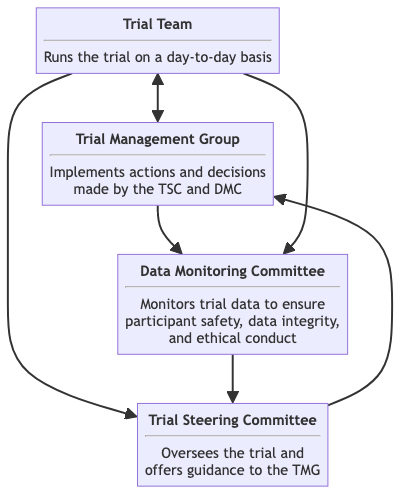
\includegraphics[width=0.6\textwidth,height=\textheight]{../shared-assets/trial-organisation-overview-figure.png}

}

\caption{\label{fig-organisation-overview}Trial organisation overview.}

\end{figure}

Trial management and oversight is governed by three trial committees and
groups: the Trial Team (TT), the Trial Management Group (TMG), the joint
Trial Steering and Data Monitoring Committee (SDMC). These groups and
their relationships are briefly described in
Figure~\ref{fig-organisation-overview}. Details about each committee and
group are available in their respective charter.

\hypertarget{trial-team}{%
\subsection{Trial team}\label{trial-team}}

\textbf{Responsibility}

To run the trial on a day-to-day basis, maintain trial databases,
randomise clusters, ensuring complete and correct data, preparing
reports for meetings (including those of the TMG and SDMC) and dealing
with research governance and, if appropriate, regulatory matters.

\textbf{Composition}

Includes the project manager, clinical research associates, principal
investigator and co-investigators as needed.

\textbf{Relationships}

Reports to the TMG and SDMC. Operationalises decisions made by the TMG.

\textbf{Meeting frequencies}

As often as needed, often weekly or bi-weekly.

\hypertarget{trial-management-group-tmg}{%
\subsection{Trial Management Group
(TMG)}\label{trial-management-group-tmg}}

\textbf{Responsibility}

To manage the trial, including its clinical and practical aspects.

\textbf{Composition}

Includes members with broad expertise appropriate to the trial. The TMG
will be chaired by the Principal Investigator.

\textbf{Relationships}

Receives reports from TT. Provides input to the SDMC. Implements
decisions made by the SDMC.

\textbf{Meeting frequencies}

Monthly to every six months.

\hypertarget{joint-trial-steering-and-data-monitoring-committee-sdmc}{%
\subsection{Joint Trial Steering and Data Monitoring Committee
(SDMC)}\label{joint-trial-steering-and-data-monitoring-committee-sdmc}}

\textbf{Responsibility}

The SDMC's responsibility is to oversee the trial, review results of
interim analyses and safety events reported by the TMG, and review trial
data for each batch, assessing data quality, completeness, cluster
performance in recruitment and loss to follow-up rates, and external
factors affecting trial validity, safety, or ethics. This committee also
offer guidance to the TMG.

\textbf{Composition}

A majority of independent members, including a chair and three
additional external experts specializing in the clinical area,
biostatistics, and a community or patient representative, as well as and
a minority of members with a direct interest in the trial, including the
principal investigator. The chair should be independent of the trial,
and the coordinating institutions Karolinska Institutet and The George
Institute for Global Health.

\textbf{Relationships}

Receives reports from the trial team and TMG.

\textbf{Meeting frequencies}

After the completion of each batch, but may be more frequent if needed.

\hypertarget{funding}{%
\section{Funding}\label{funding}}

\begin{itemize}
\tightlist
\item
  Swedish Research Council (reg. no. 2023-03128)
\item
  Laerdal Foundation (reg. no. 2023-0297)
\end{itemize}

\hypertarget{special-considerations}{%
\section{Special considerations}\label{special-considerations}}

\hypertarget{funding-1}{%
\subsection{Funding}\label{funding-1}}

This trial is not yet fully funded. The Trial Management Group has
decided to proceed with the trial with the expectation that additional
funding will be secured. The Trial Steering Committee will be informed
of the funding status at each meeting. If funding is not secured, the
trial will be stopped. This will likely result in an underpowered trial.
The justification for this decision is that the intervention is
considered standard of care in many countries and the data collection is
considered minimal risk. There is therefore a very small risk of harm to
patient participants, but a potential direct benefit to those patient
participants who receive the intervention. The benefit-risk ratio is
therefore considered to be favourable, even in the case of an
underpowered trial.

\hypertarget{potential-amendments}{%
\subsection{Potential amendments}\label{potential-amendments}}

There are ongoing discussions about re-framing the trial as a hybrid
effectiveness-implementation trial and include a cost-effectiveness
analysis. This would involve adding additional data collection to assess
the implementation and costs of the intervention. This would involve
additional funding and amended ethical approvals.

\hypertarget{notification-of-trial-completion-reporting-and-publication}{%
\section{Notification of trial completion, reporting, and
publication}\label{notification-of-trial-completion-reporting-and-publication}}

The trial will be reported to the Funders within a year of completion.
The results of the trial will also be prepared as manuscripts for
publication. Authorship on trial manuscripts will be based on the
International Committee of Medical Journal Editors (ICMJE)
criteria\textsuperscript{43}:

\begin{quote}
\begin{itemize}
\tightlist
\item
  Substantial contributions to the conception or design of the work; or
  the acquisition, analysis, or interpretation of data for the work; AND
\item
  Drafting the work or reviewing it critically for important
  intellectual content; AND
\item
  Final approval of the version to be published; AND
\item
  Agreement to be accountable for all aspects of the work in ensuring
  that questions related to the accuracy or integrity of any part of the
  work are appropriately investigated and resolved.
\end{itemize}

In addition to being accountable for the parts of the work done, an
author should be able to identify which co-authors are responsible for
specific other parts of the work. In addition, authors should have
confidence in the integrity of the contributions of their co-authors.
\end{quote}

The most recent version of the ICMJE criteria will be adhered to. We
will also use the ICMJE criteria for non-author contributorship.

Before work on a trial manuscript is initiated, a writing group will be
formed and first and last authors will be designated. This writing group
will be formed by discussion in the Trial Management Group.

\hypertarget{references}{%
\section{References}\label{references}}

\hypertarget{refs}{}
\begin{CSLReferences}{0}{0}
\leavevmode\vadjust pre{\hypertarget{ref-injuries2020}{}}%
\CSLLeftMargin{1. }%
\CSLRightInline{GBD 2019 Diseases and Injuries Collaborators.
Injuries---level 1 cause. \emph{The Lancet} \textbf{396}, (2020).}

\leavevmode\vadjust pre{\hypertarget{ref-GBD2020}{}}%
\CSLLeftMargin{2. }%
\CSLRightInline{GBD 2019 Diseases and Injuries Collaborators. Global
burden of 369 diseases and injuries in 204 countries and territories,
1990--2019: A systematic analysis for the global burden of disease study
2019. \emph{The Lancet} \textbf{396}, 1204--1222 (2020).}

\leavevmode\vadjust pre{\hypertarget{ref-Rauf2019}{}}%
\CSLLeftMargin{3. }%
\CSLRightInline{Rauf, R. \emph{et al.} Changes in the temporal
distribution of in-hospital mortality in severely injured patients---an
analysis of the TraumaRegister DGU. \emph{PLOS ONE} \textbf{14},
e0212095 (2019).}

\leavevmode\vadjust pre{\hypertarget{ref-Roy2017}{}}%
\CSLLeftMargin{4. }%
\CSLRightInline{Roy, N. \emph{et al.} Learning from 2523 trauma deaths
in india- opportunities to prevent in-hospital deaths. \emph{BMC Health
Serv Res} \textbf{17}, (2017).}

\leavevmode\vadjust pre{\hypertarget{ref-Callcut2019}{}}%
\CSLLeftMargin{5. }%
\CSLRightInline{Callcut, R. A. \emph{et al.} The why and how our trauma
patients die: A prospective multicenter western trauma association
study. \emph{J Trauma.} \textbf{86}, 864--870 (2019).}

\leavevmode\vadjust pre{\hypertarget{ref-Ghorbani2018}{}}%
\CSLLeftMargin{6. }%
\CSLRightInline{Ghorbani, P. \emph{et al.} Analysis of preventable
deaths and errors in trauma care in a scandinavian trauma level-i
centre. \emph{Acta Anaesthesiol Scand} \textbf{62}, 1146--1153 (2018).}

\leavevmode\vadjust pre{\hypertarget{ref-Mohammad2013}{}}%
\CSLLeftMargin{7. }%
\CSLRightInline{Mohammad, A. \emph{et al.} Educational and clinical
impact of advanced trauma life support (ATLS) courses: A systematic
review. \emph{World J. Surg.} \textbf{38}, 322--329 (2013).}

\leavevmode\vadjust pre{\hypertarget{ref-Jayaraman2014}{}}%
\CSLLeftMargin{8. }%
\CSLRightInline{Jayaraman, S. \emph{et al.} Advanced trauma life support
training for hospital staff. \emph{Cochrane Database Syst Rev} (2014).}

\leavevmode\vadjust pre{\hypertarget{ref-Kadhum2020}{}}%
\CSLLeftMargin{9. }%
\CSLRightInline{Kadhum, M. \emph{et al.} Are primary trauma care (PTC)
courses beneficial in low- and middle-income countries - a systematic
review. \emph{Injury} \textbf{51}, 136--141 (2020).}

\leavevmode\vadjust pre{\hypertarget{ref-Jin2021}{}}%
\CSLLeftMargin{10. }%
\CSLRightInline{Jin, J. \emph{et al.} Effectiveness of quality
improvement processes, interventions, and structure in trauma systems in
low- and middle-income countries: A systematic review and meta-analysis.
\emph{World J. Surg.} \textbf{45}, 1982--1998 (2021).}

\leavevmode\vadjust pre{\hypertarget{ref-mciver_effect_2024}{}}%
\CSLLeftMargin{11. }%
\CSLRightInline{McIver, R. \emph{et al.} Effect of trauma quality
improvement initiatives on outcomes and costs at community hospitals:
{A} scoping review. \emph{Injury} \textbf{55}, 111492 (2024).}

\leavevmode\vadjust pre{\hypertarget{ref-acsAtls2018}{}}%
\CSLLeftMargin{12. }%
\CSLRightInline{Committee on Trauma. \emph{Advanced trauma life support®
student course manual}. (American College of Surgeons, 2018).}

\leavevmode\vadjust pre{\hypertarget{ref-ACS2022}{}}%
\CSLLeftMargin{13. }%
\CSLRightInline{American College of Surgeons. \emph{Resources for
optimal care of the injured patient}. ({American College of Surgeons},
2022).}

\leavevmode\vadjust pre{\hypertarget{ref-Ali1995}{}}%
\CSLLeftMargin{14. }%
\CSLRightInline{Ali, J. \emph{et al.} Demonstration of acquisition of
trauma management skills by senior medical students completing the ATLS
program. \emph{J Trauma.} \textbf{38}, 687--691 (1995).}

\leavevmode\vadjust pre{\hypertarget{ref-Ali1996}{}}%
\CSLLeftMargin{15. }%
\CSLRightInline{Ali, J. \emph{et al.} Teaching effectiveness of the
advanced trauma life support program as demonstrated by an objective
structured clinical examination for practicing physicians. \emph{World
J. Surg.} \textbf{20}, 1121--1126 (1996).}

\leavevmode\vadjust pre{\hypertarget{ref-Ali1999}{}}%
\CSLLeftMargin{16. }%
\CSLRightInline{Ali, J. \emph{et al.} Comparison of performance of
interns completing the old (1993) and new interactive (1997) advanced
trauma life support courses. \emph{J Trauma.} \textbf{46}, 80--86
(1999).}

\leavevmode\vadjust pre{\hypertarget{ref-putra_impact_2023}{}}%
\CSLLeftMargin{17. }%
\CSLRightInline{Putra, A. B. \emph{et al.} Impact of {Advanced} {Trauma}
{Life} {Support} {Training} for {Improving} {Mortality} {Outcome}: {A}
{Systematic} {Review} and {Meta}-analysis. \emph{The New Ropanasury
Journal of Surgery} \textbf{8}, (2023).}

\leavevmode\vadjust pre{\hypertarget{ref-Vestrup1988}{}}%
\CSLLeftMargin{18. }%
\CSLRightInline{Vestrup, J. A. \emph{et al.} Impact of advanced trauma
life support training on early trauma management. \emph{Am J Surg}
\textbf{155}, 704--707 (1988).}

\leavevmode\vadjust pre{\hypertarget{ref-Ariyanayagam1992}{}}%
\CSLLeftMargin{19. }%
\CSLRightInline{Ariyanayagam, D. C. \emph{et al.} The impact of the ATLS
course on traffic accident mortality in trinidad and tobago. \emph{West
Indian Med J} \textbf{41}, 72--74 (1992).}

\leavevmode\vadjust pre{\hypertarget{ref-Ali1993}{}}%
\CSLLeftMargin{20. }%
\CSLRightInline{Ali, J. \emph{et al.} Trauma outcome improves following
the advanced trauma life support program in a developing country.
\emph{J Trauma} \textbf{34}, 890--899 (1993).}

\leavevmode\vadjust pre{\hypertarget{ref-Olson2001}{}}%
\CSLLeftMargin{21. }%
\CSLRightInline{Olson, C. J. \emph{et al.} Influence of trauma system
implementation on process of care delivered to seriously injured
patients in rural trauma centers. \emph{Surgery} \textbf{130}, 273--279
(2001).}

\leavevmode\vadjust pre{\hypertarget{ref-vanOlden2004}{}}%
\CSLLeftMargin{22. }%
\CSLRightInline{Olden, G. D. J. van \emph{et al.} Clinical impact of
advanced trauma life support. \emph{Am J Emerg Med} \textbf{22},
522--525 (2004).}

\leavevmode\vadjust pre{\hypertarget{ref-Wang2010}{}}%
\CSLLeftMargin{23. }%
\CSLRightInline{Wang, P. \emph{et al.} Comparison of severe trauma care
effect before and after advanced trauma life support training.
\emph{Chin J Traumatol} \textbf{13}, 341--344 (2010).}

\leavevmode\vadjust pre{\hypertarget{ref-Drimousis2011}{}}%
\CSLLeftMargin{24. }%
\CSLRightInline{Drimousis, P. G. \emph{et al.} Advanced trauma life
support certified physicians in a non trauma system setting: Is it
enough? \emph{Resuscitation} \textbf{82}, 180--184 (2011).}

\leavevmode\vadjust pre{\hypertarget{ref-Hashmi2013}{}}%
\CSLLeftMargin{25. }%
\CSLRightInline{Hashmi, Z. G. \emph{et al.} Hospital-based trauma
quality improvement initiatives. \emph{J Trauma} \textbf{75}, 60--68
(2013).}

\leavevmode\vadjust pre{\hypertarget{ref-Petroze2014}{}}%
\CSLLeftMargin{26. }%
\CSLRightInline{Petroze, R. T. \emph{et al.} Can focused trauma
education initiatives reduce mortality or improve resource utilization
in a low-resource setting? \emph{World J. Surg.} \textbf{39}, 926--933
(2014).}

\leavevmode\vadjust pre{\hypertarget{ref-Bellanova2016}{}}%
\CSLLeftMargin{27. }%
\CSLRightInline{Giovanni Bellanova, R. B., Francesco Buccelletti. How
formative courses about damage control surgery and non-operative
management improved outcome and survival in unstable politrauma patients
in a mountain trauma center. \emph{Annali italiani di chirurgia}
\textbf{87}, 68--74 (2016).}

\leavevmode\vadjust pre{\hypertarget{ref-GerdinWuxe4rnberg2022}{}}%
\CSLLeftMargin{28. }%
\CSLRightInline{Gerdin Wärnberg, M. \emph{et al.} A pilot multicentre
cluster randomised trial to compare the effect of trauma life support
training programmes on patient and provider outcomes. \emph{BMJ Open}
\textbf{12}, e057504 (2022).}

\leavevmode\vadjust pre{\hypertarget{ref-Hemming2015}{}}%
\CSLLeftMargin{29. }%
\CSLRightInline{Hemming, K. \emph{et al.} The stepped wedge cluster
randomised trial: Rationale, design, analysis, and reporting. \emph{BMJ}
\textbf{350}, h391--h391 (2015).}

\leavevmode\vadjust pre{\hypertarget{ref-Hemming2020May}{}}%
\CSLLeftMargin{30. }%
\CSLRightInline{Hemming, K. \emph{et al.} Reflection on modern methods:
When is a stepped-wedge cluster randomized trial a good study design
choice? \emph{Int J Epidemiol} \textbf{49}, 1043--1052 (2020).}

\leavevmode\vadjust pre{\hypertarget{ref-Kasza2022}{}}%
\CSLLeftMargin{31. }%
\CSLRightInline{Kasza, J. \emph{et al.} The batched stepped wedge
design: A design robust to delays in cluster recruitment. \emph{Stat
Med} \textbf{41}, 3627--3641 (2022).}

\leavevmode\vadjust pre{\hypertarget{ref-harris_research_2009}{}}%
\CSLLeftMargin{32. }%
\CSLRightInline{Harris, P. A. \emph{et al.} Research electronic data
capture ({REDCap})--a metadata-driven methodology and workflow process
for providing translational research informatics support. \emph{Journal
of Biomedical Informatics} \textbf{42}, 377--381 (2009).}

\leavevmode\vadjust pre{\hypertarget{ref-harris_redcap_2019}{}}%
\CSLLeftMargin{33. }%
\CSLRightInline{Harris, P. A. \emph{et al.} The {REDCap} consortium:
{Building} an international community of software platform partners.
\emph{Journal of Biomedical Informatics} \textbf{95}, 103208 (2019).}

\leavevmode\vadjust pre{\hypertarget{ref-aukstakalnis_impact_2024}{}}%
\CSLLeftMargin{34. }%
\CSLRightInline{Aukstakalnis, V. \emph{et al.} Impact of video
recordings review with structured debriefings on trauma team
performance: A prospective observational cohort study. \emph{European
Journal of Trauma and Emergency Surgery: Official Publication of the
European Trauma Society} (2024).}

\leavevmode\vadjust pre{\hypertarget{ref-STEPCARE2023}{}}%
\CSLLeftMargin{35. }%
\CSLRightInline{Nielsen, Niklas. Sedation, {Temperature} and {Pressure}
after {Cardiac} {Arrest} and {Resuscitation} -- the {STEPCARE} trial.
(2023).}

\leavevmode\vadjust pre{\hypertarget{ref-Diaz2021}{}}%
\CSLLeftMargin{36. }%
\CSLRightInline{Diaz, T. \emph{et al.} A call for standardised
age-disaggregated health data. \emph{The Lancet Healthy Longevity}
\textbf{2}, e436--e443 (2021).}

\leavevmode\vadjust pre{\hypertarget{ref-Li2020}{}}%
\CSLLeftMargin{37. }%
\CSLRightInline{Li, F. \emph{et al.} Mixed-effects models for the design
and analysis of stepped wedge cluster randomized trials: An overview.
\emph{Stat Methods Med Res} \textbf{30}, 612--639 (2020).}

\leavevmode\vadjust pre{\hypertarget{ref-Campbell2005}{}}%
\CSLLeftMargin{38. }%
\CSLRightInline{Campbell, M. K. \emph{et al.} Determinants of the
intracluster correlation coefficient in cluster randomized trials: The
case of implementation research. \emph{Clinical Trials} \textbf{2},
99--107 (2005).}

\leavevmode\vadjust pre{\hypertarget{ref-Eldridge2015}{}}%
\CSLLeftMargin{39. }%
\CSLRightInline{Eldridge, S. M. \emph{et al.} How big should the pilot
study for my cluster randomised trial be? \emph{Stat Methods Med Res}
\textbf{25}, 1039--1056 (2015).}

\leavevmode\vadjust pre{\hypertarget{ref-Hemming2020Feb}{}}%
\CSLLeftMargin{40. }%
\CSLRightInline{Hemming, K. \emph{et al.} A tutorial on sample size
calculation for multiple-period cluster randomized parallel, cross-over
and stepped-wedge trials using the shiny CRT calculator. \emph{Int J
Epidemiol} \textbf{49}, 979--995 (2020).}

\leavevmode\vadjust pre{\hypertarget{ref-Martin2016}{}}%
\CSLLeftMargin{41. }%
\CSLRightInline{Martin, J. \emph{et al.} Intra-cluster and inter-period
correlation coefficients for cross-sectional cluster randomised
controlled trials for type-2 diabetes in UK primary care. \emph{Trials}
\textbf{17}, (2016).}

\leavevmode\vadjust pre{\hypertarget{ref-Korevaar2021}{}}%
\CSLLeftMargin{42. }%
\CSLRightInline{Korevaar, E. \emph{et al.} Intra-cluster correlations
from the CLustered OUtcome dataset bank to inform the design of
longitudinal cluster trials. \emph{Clinical Trials} \textbf{18},
529--540 (2021).}

\leavevmode\vadjust pre{\hypertarget{ref-icmje_2024}{}}%
\CSLLeftMargin{43. }%
\CSLRightInline{{ICMJE} {\textbar} {Recommendations} {\textbar}
{Defining} the {Role} of {Authors} and {Contributors}.}

\end{CSLReferences}

\hypertarget{appendices}{%
\section{Appendices}\label{appendices}}

\hypertarget{sec-appendix-hospital-screening-instrument}{%
\subsection{Initial hospital screening
instrument}\label{sec-appendix-hospital-screening-instrument}}

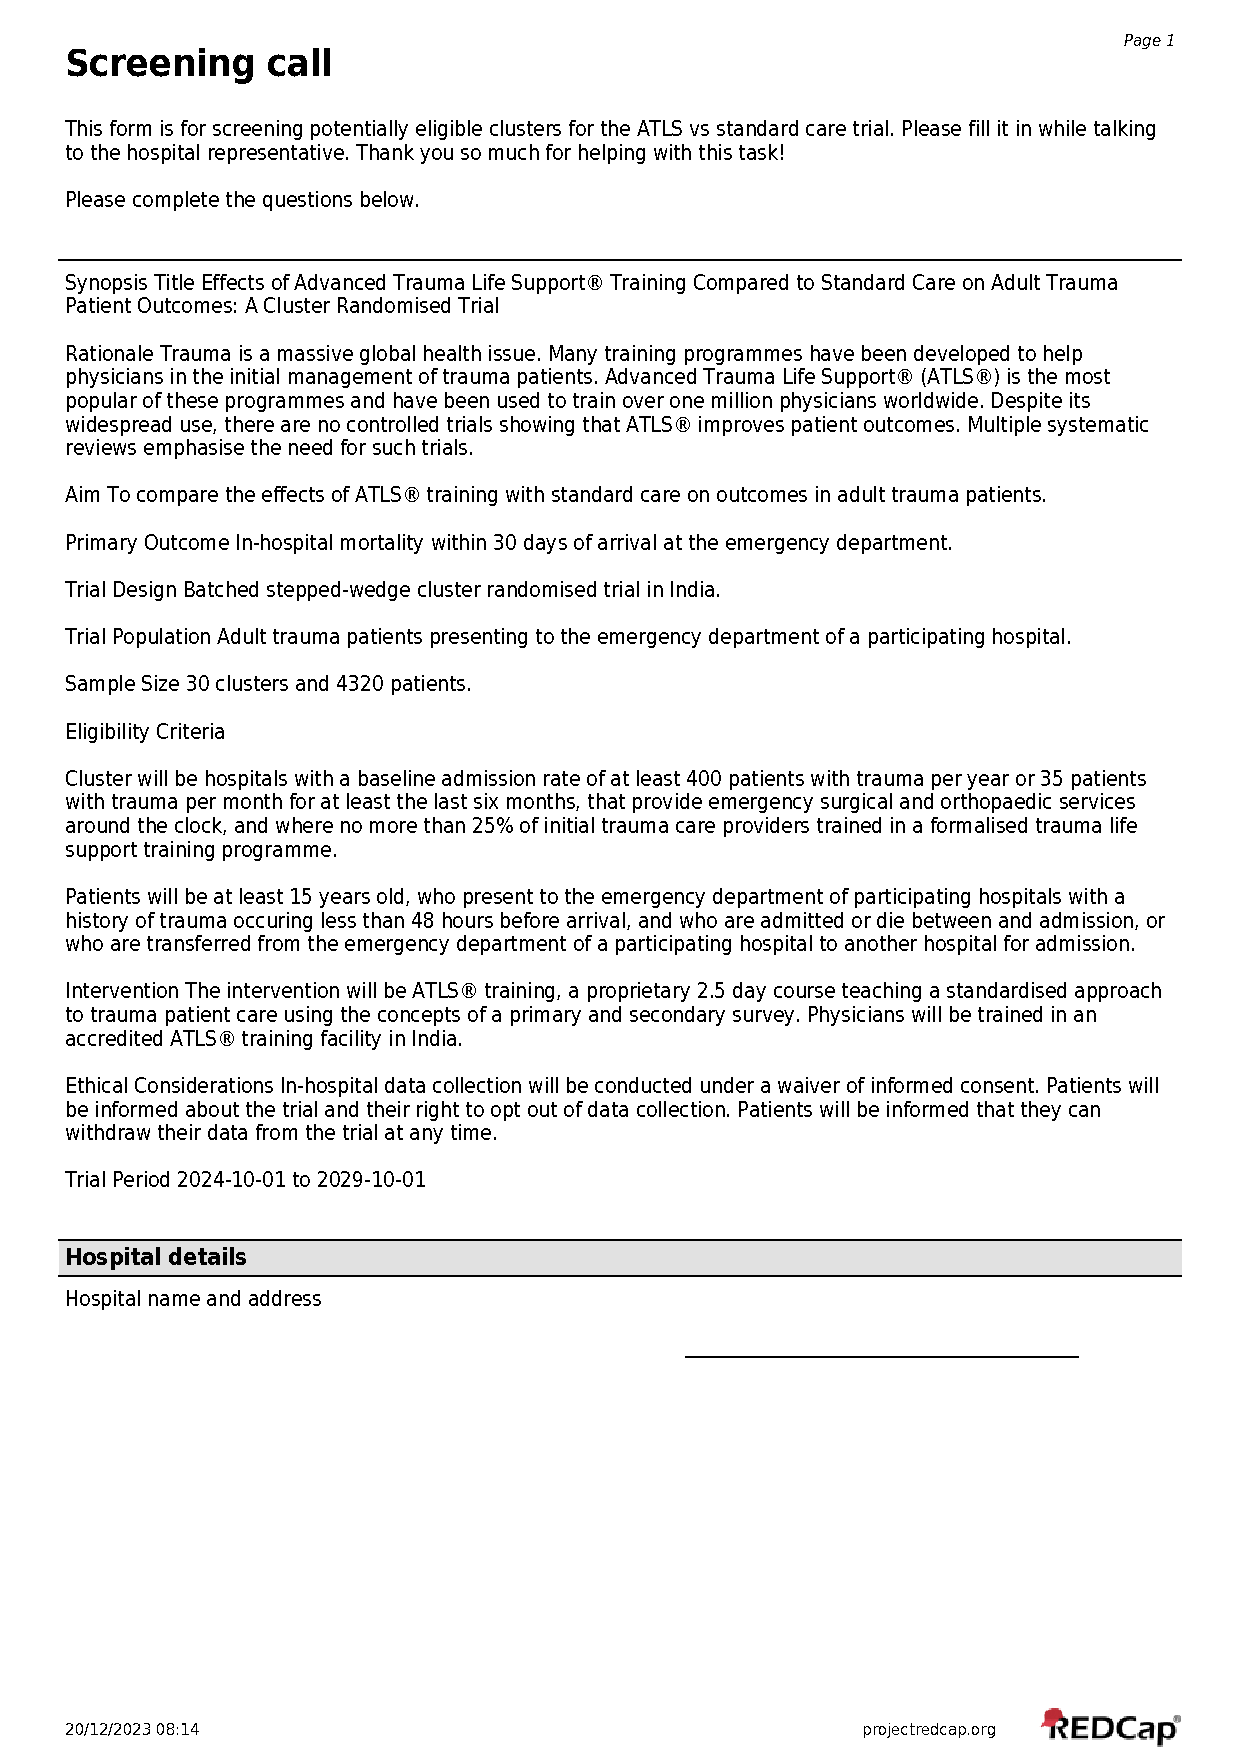
\includegraphics{./appendices/hospital-screening-instrument/hospital-screening-instrument-1.pdf}

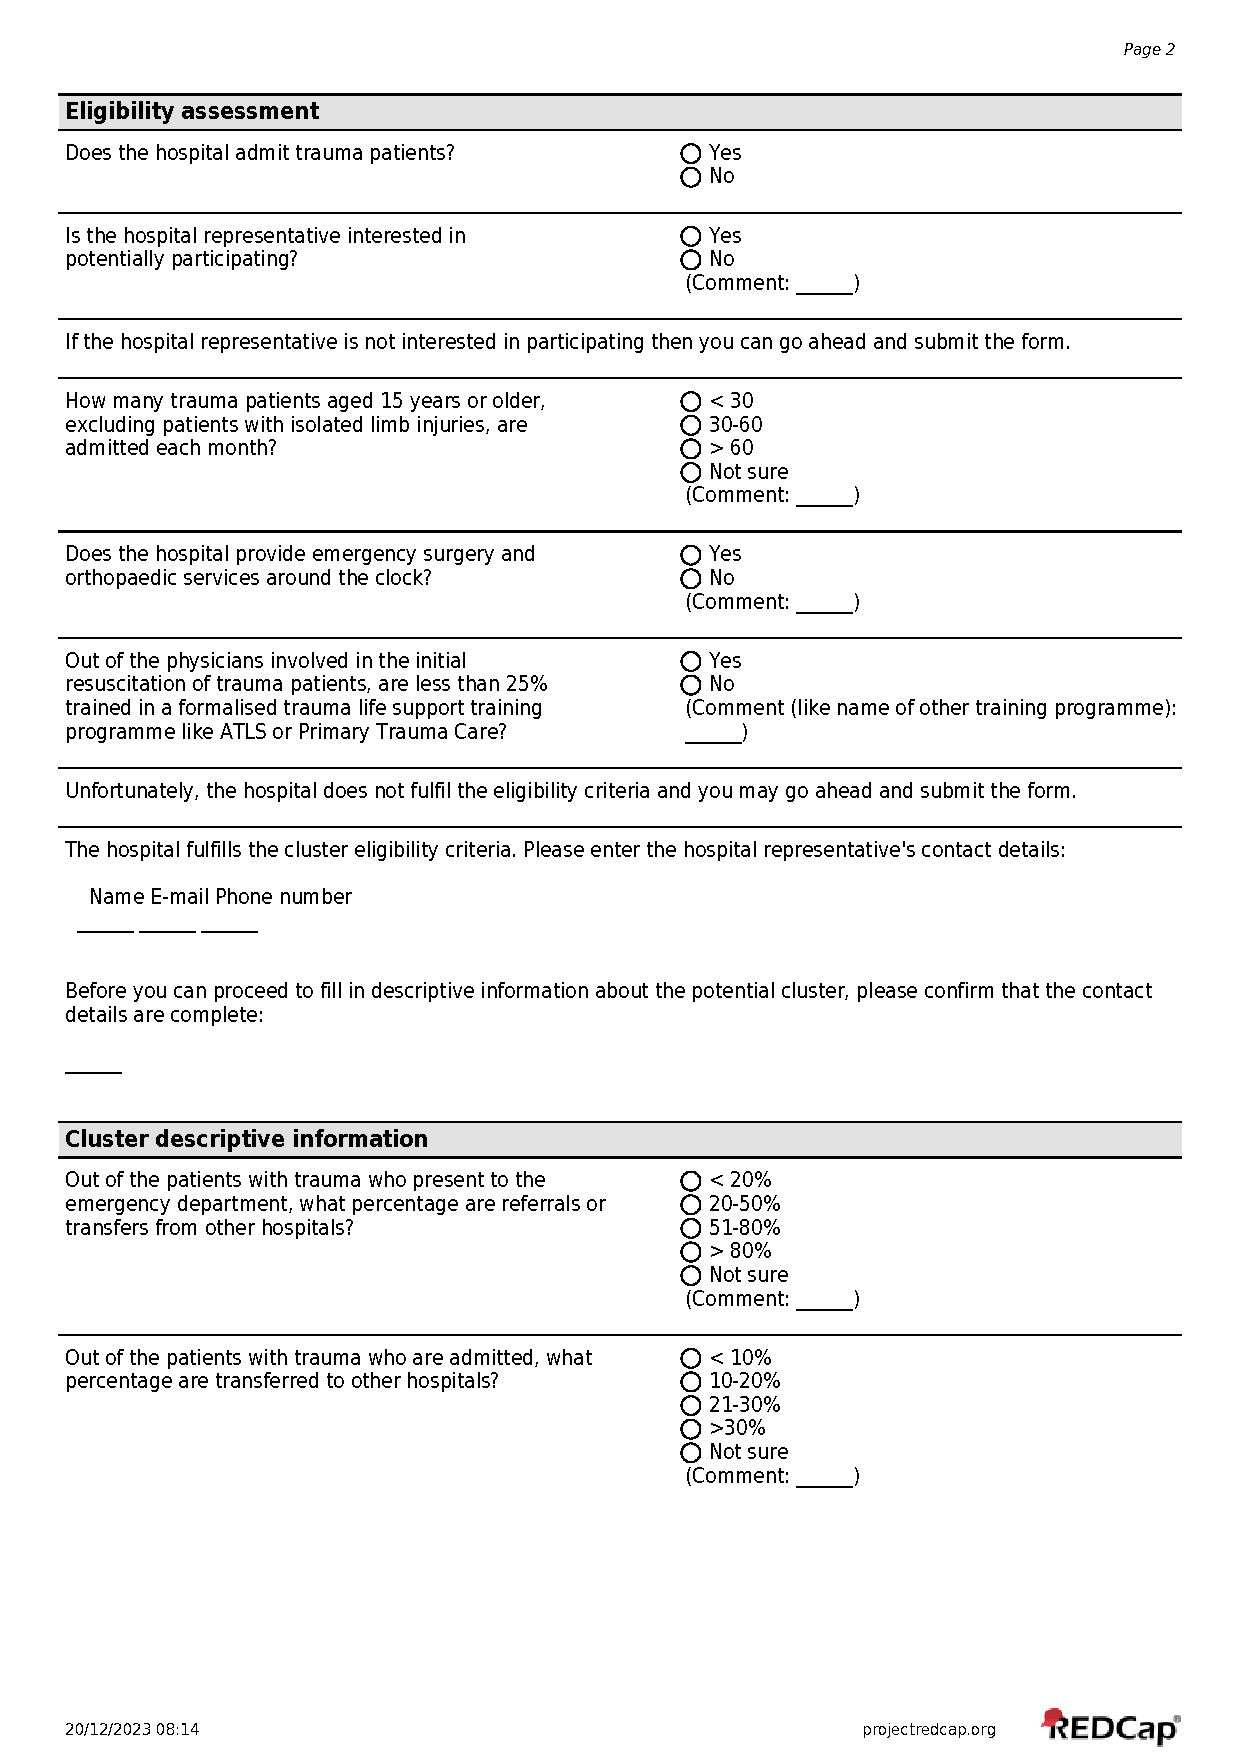
\includegraphics{./appendices/hospital-screening-instrument/hospital-screening-instrument-2.pdf}

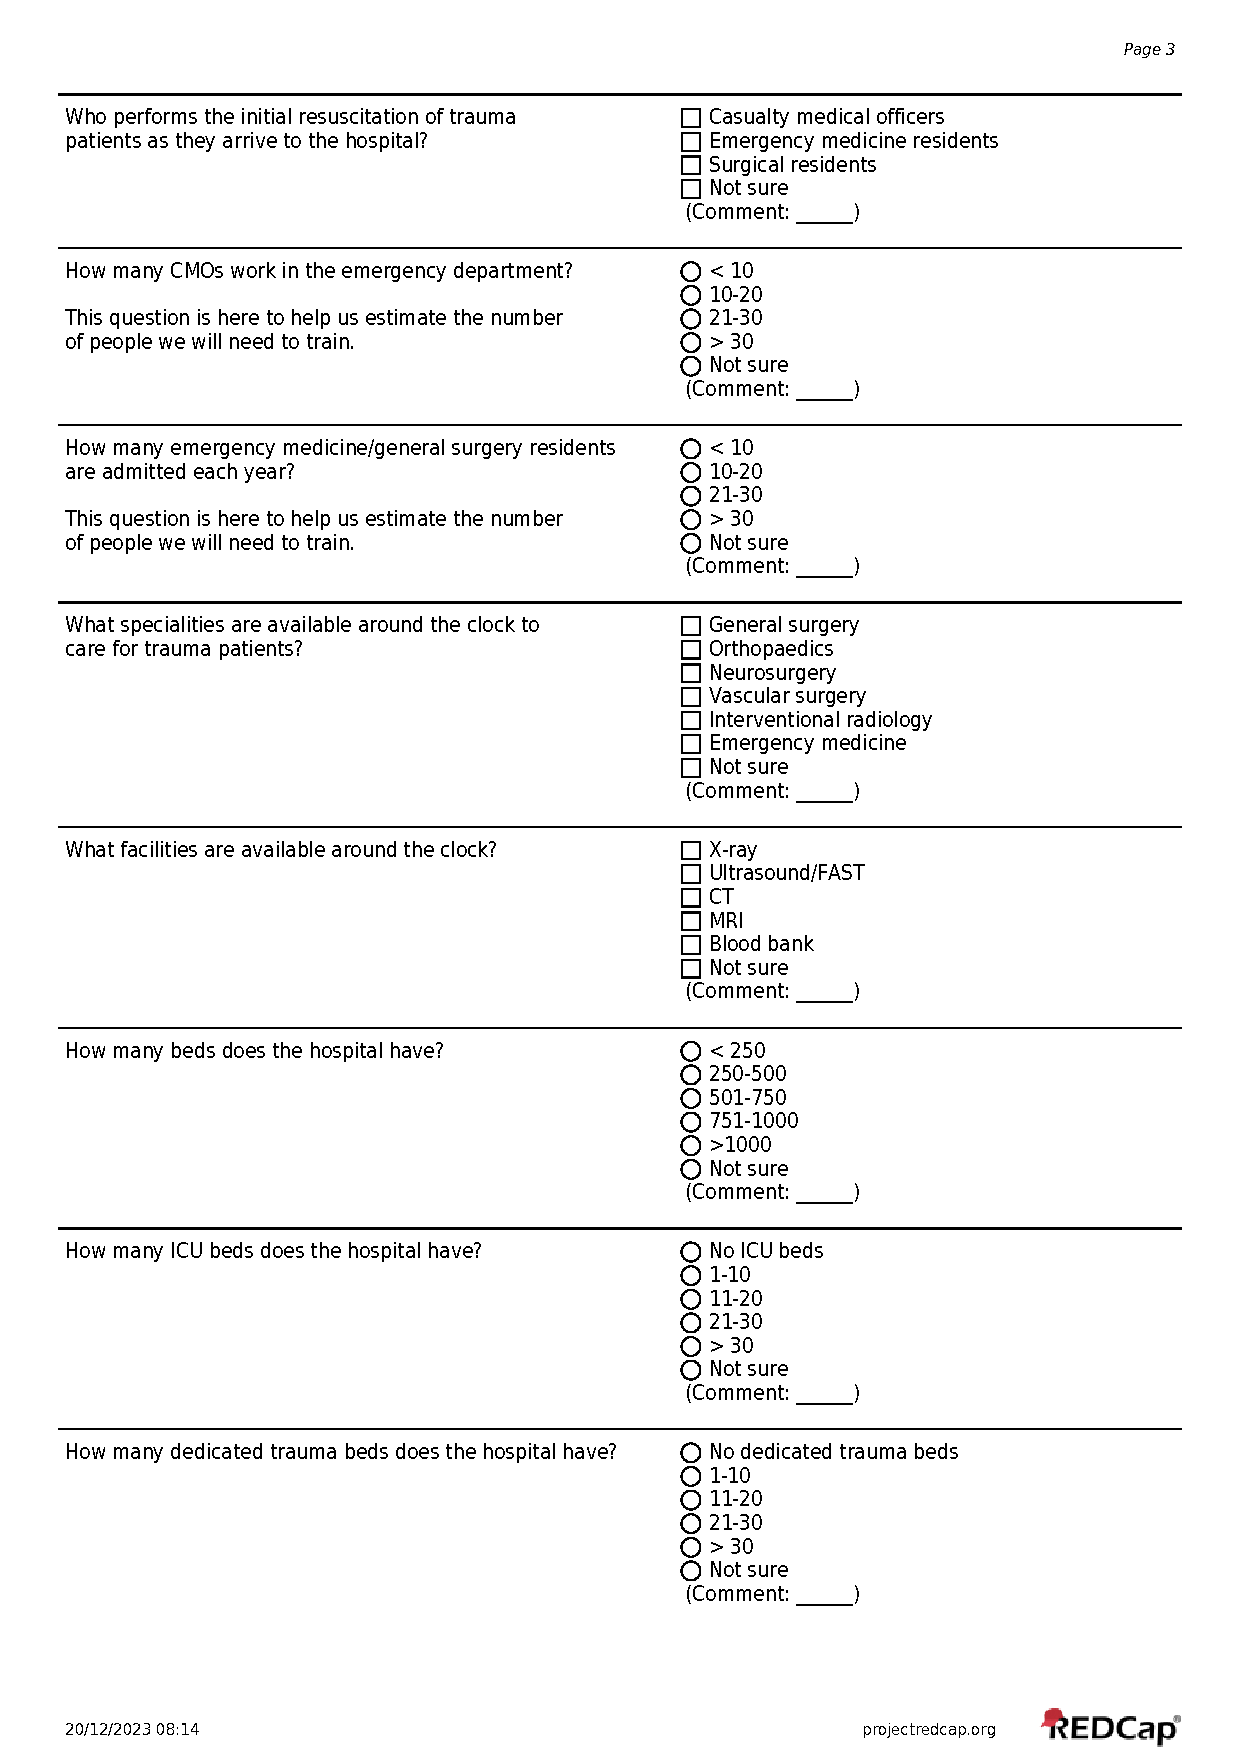
\includegraphics{./appendices/hospital-screening-instrument/hospital-screening-instrument-3.pdf}


\includegraphics{./appendices/hospital-screening-instrument/hospital-screening-instrument-4.pdf}

\hypertarget{sec-appendix-hospital-screening-interview-instrument}{%
\subsection{In-depth hospital screening interview
instrument}\label{sec-appendix-hospital-screening-interview-instrument}}

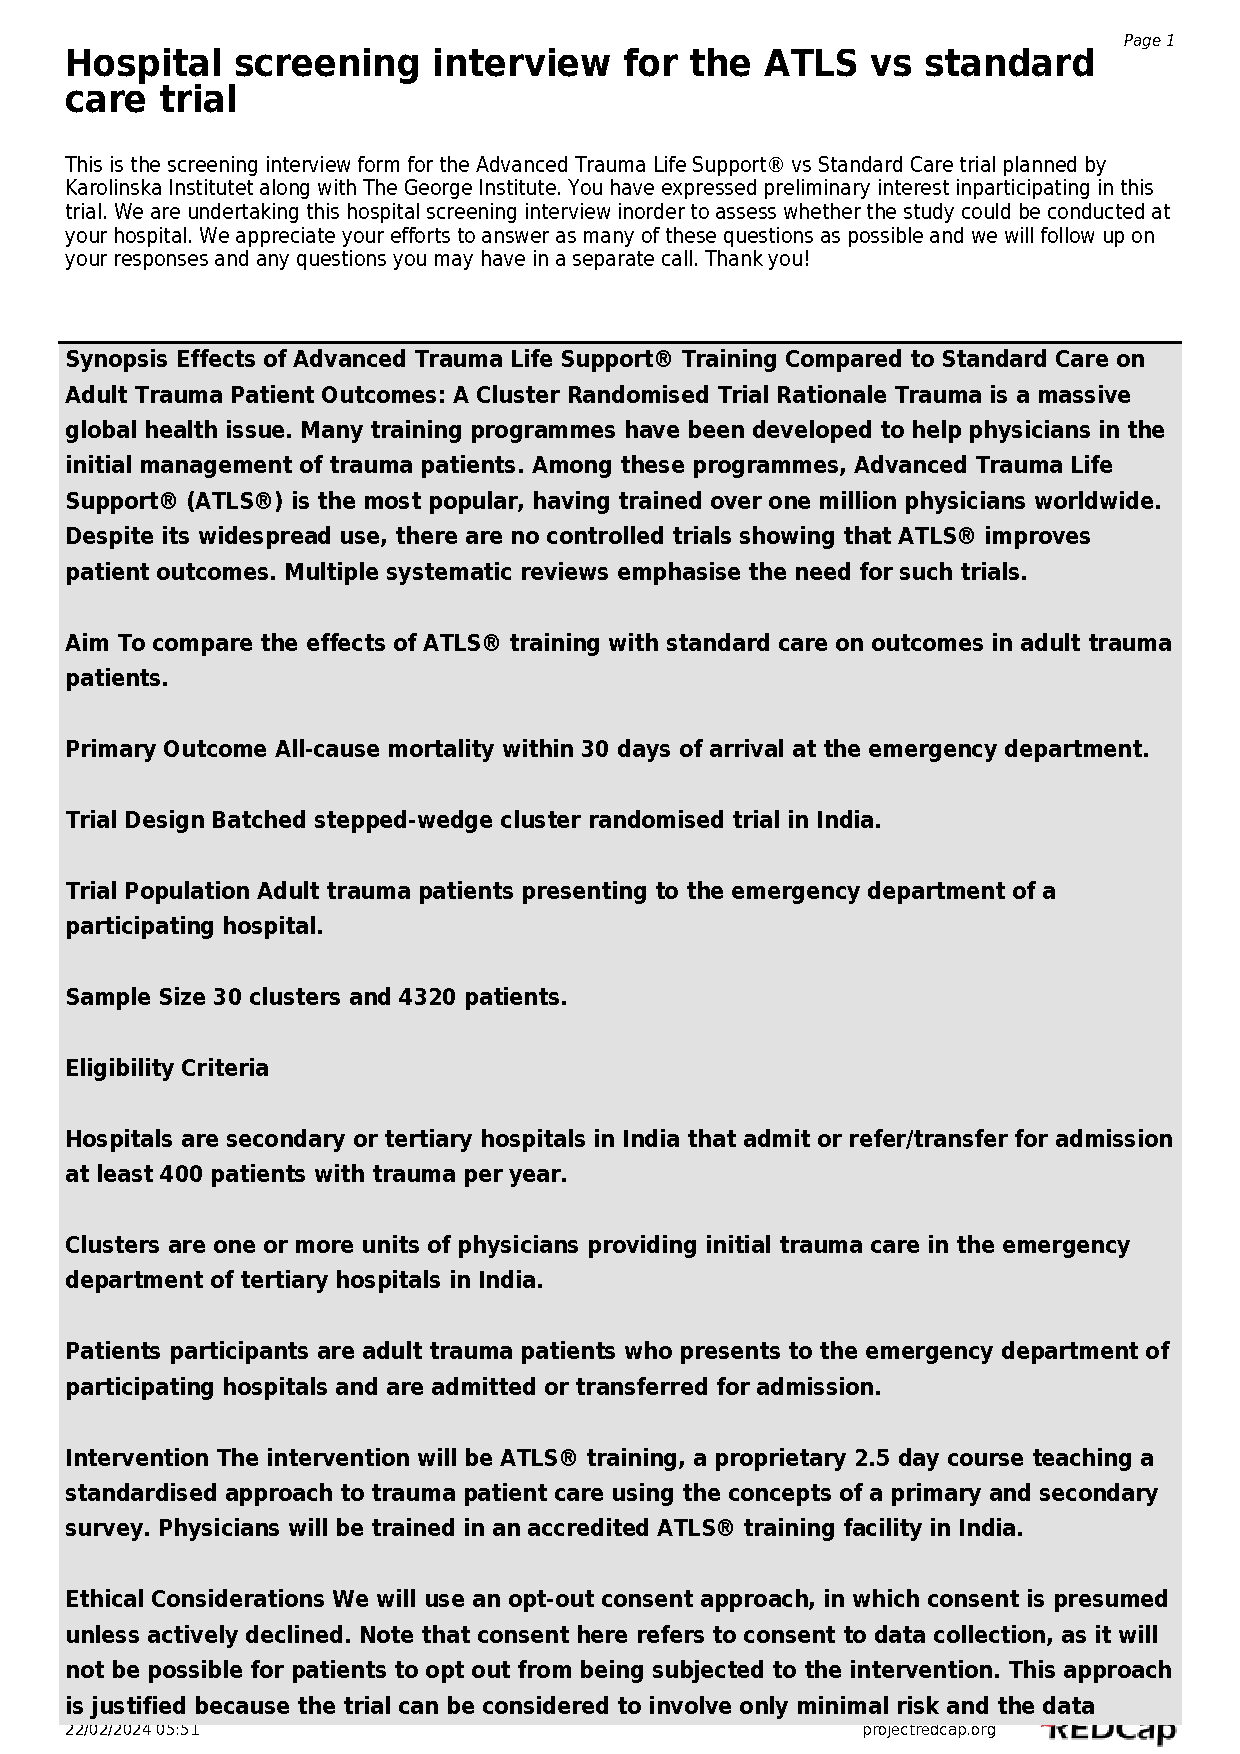
\includegraphics{./appendices/hospital-screening-interview-instrument/hospital-screening-interview-1.pdf}

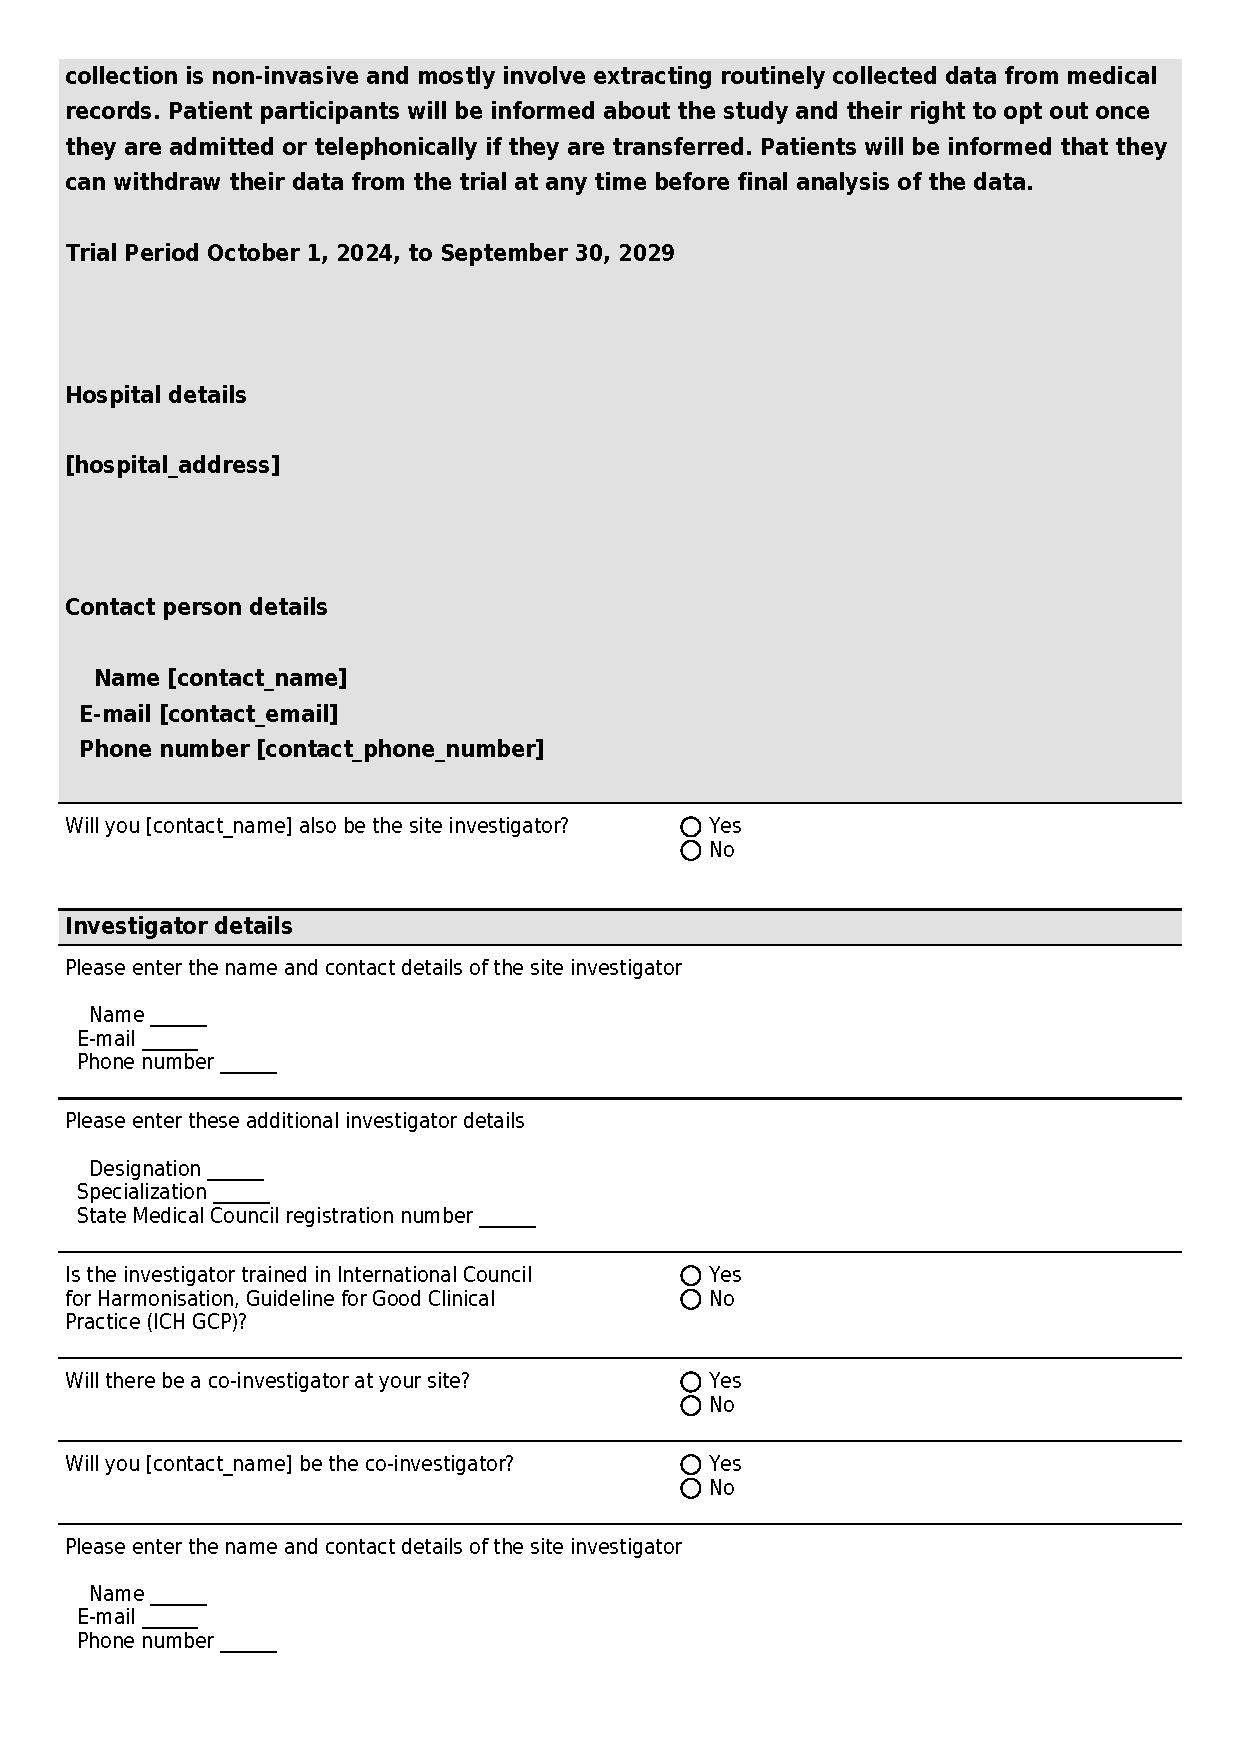
\includegraphics{./appendices/hospital-screening-interview-instrument/hospital-screening-interview-2.pdf}

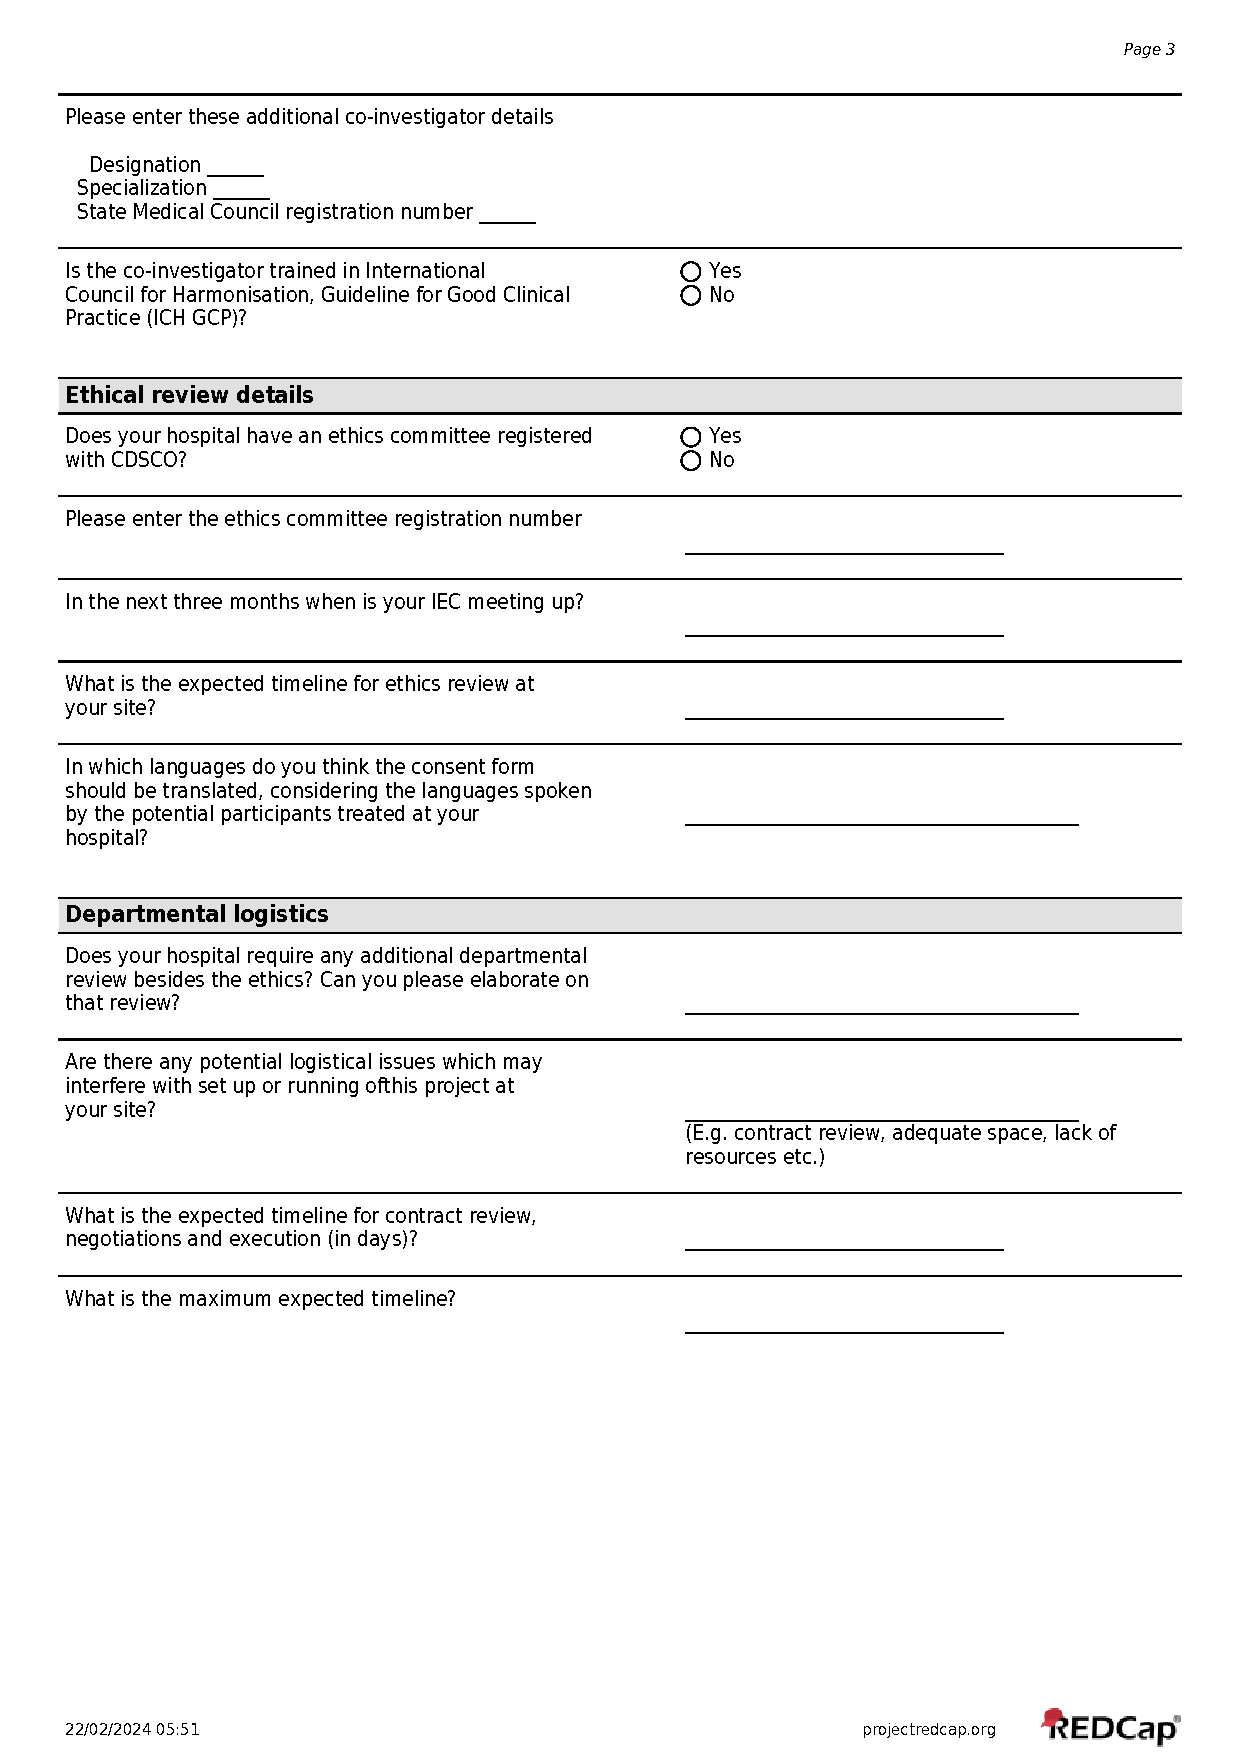
\includegraphics{./appendices/hospital-screening-interview-instrument/hospital-screening-interview-3.pdf}

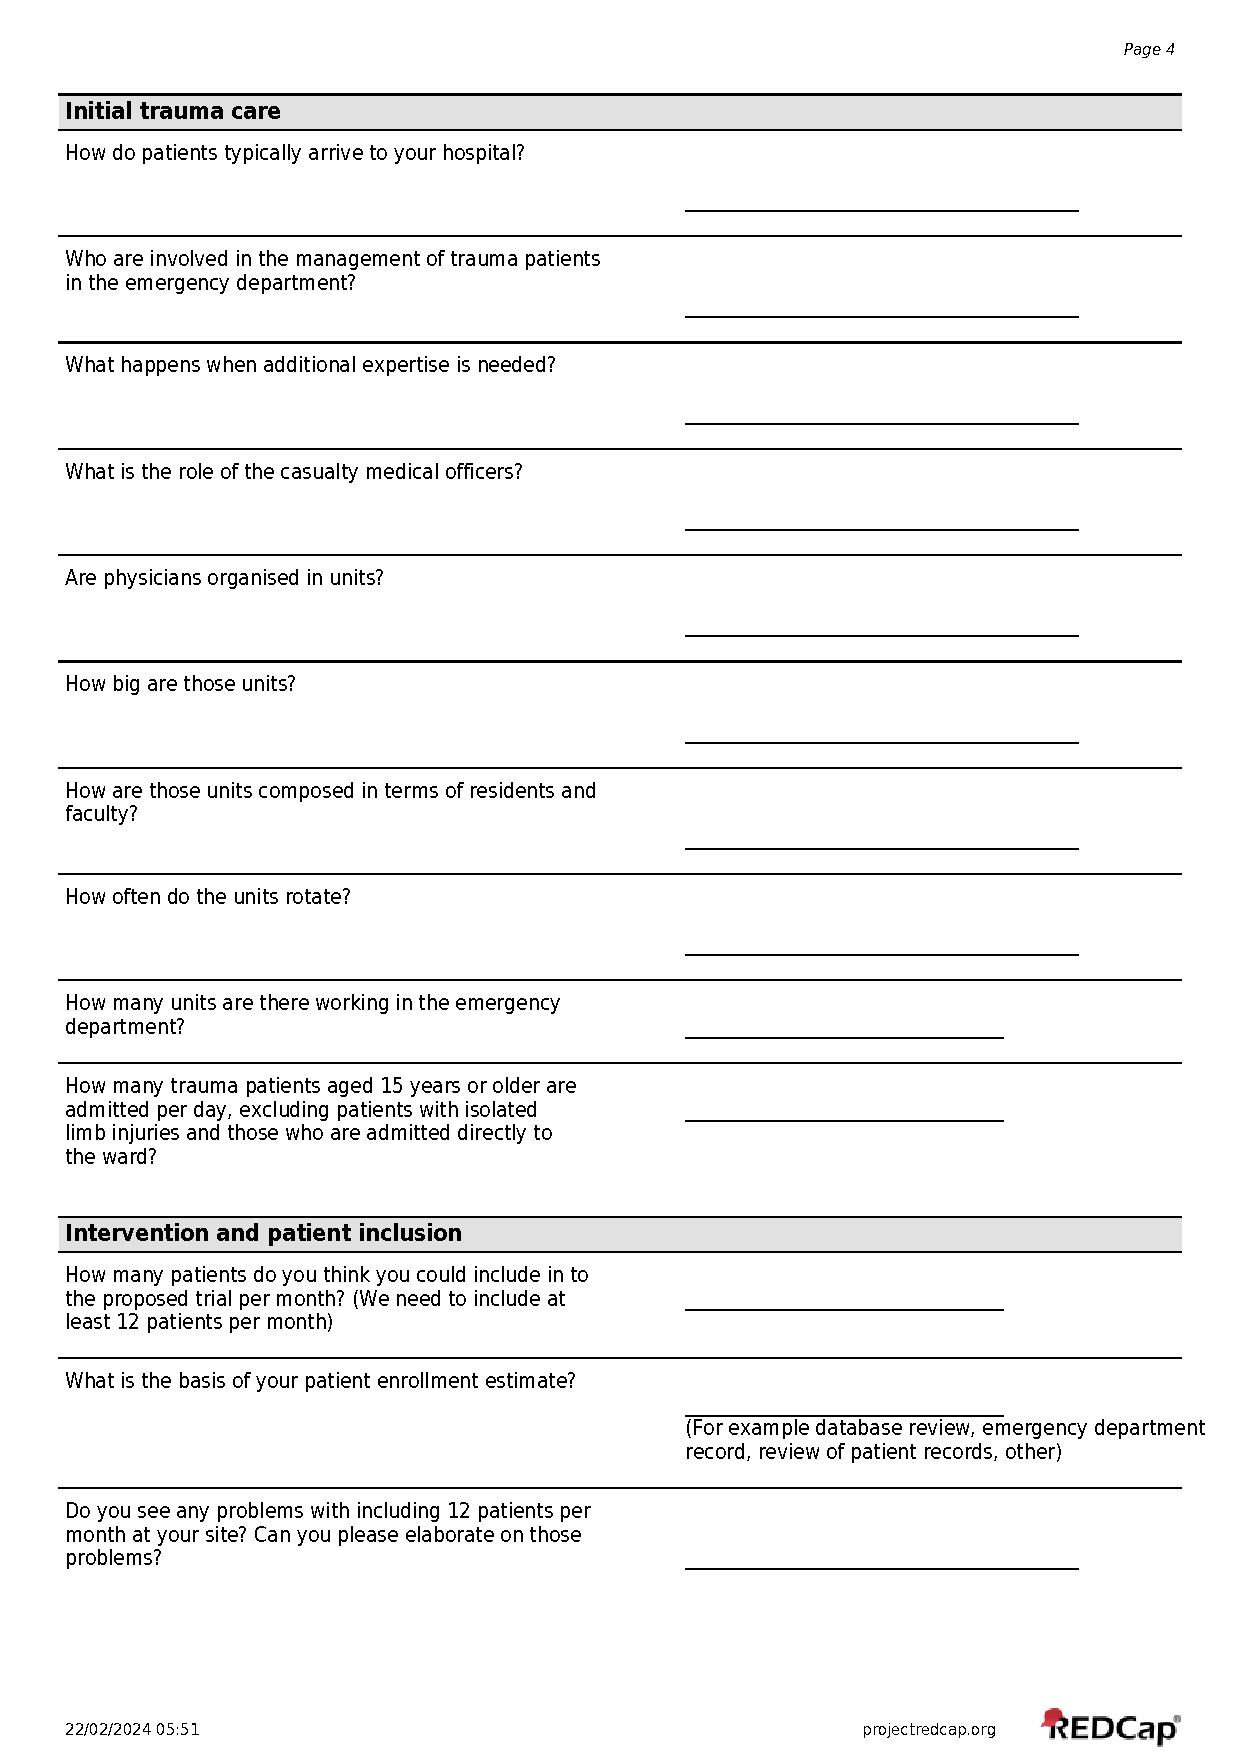
\includegraphics{./appendices/hospital-screening-interview-instrument/hospital-screening-interview-4.pdf}

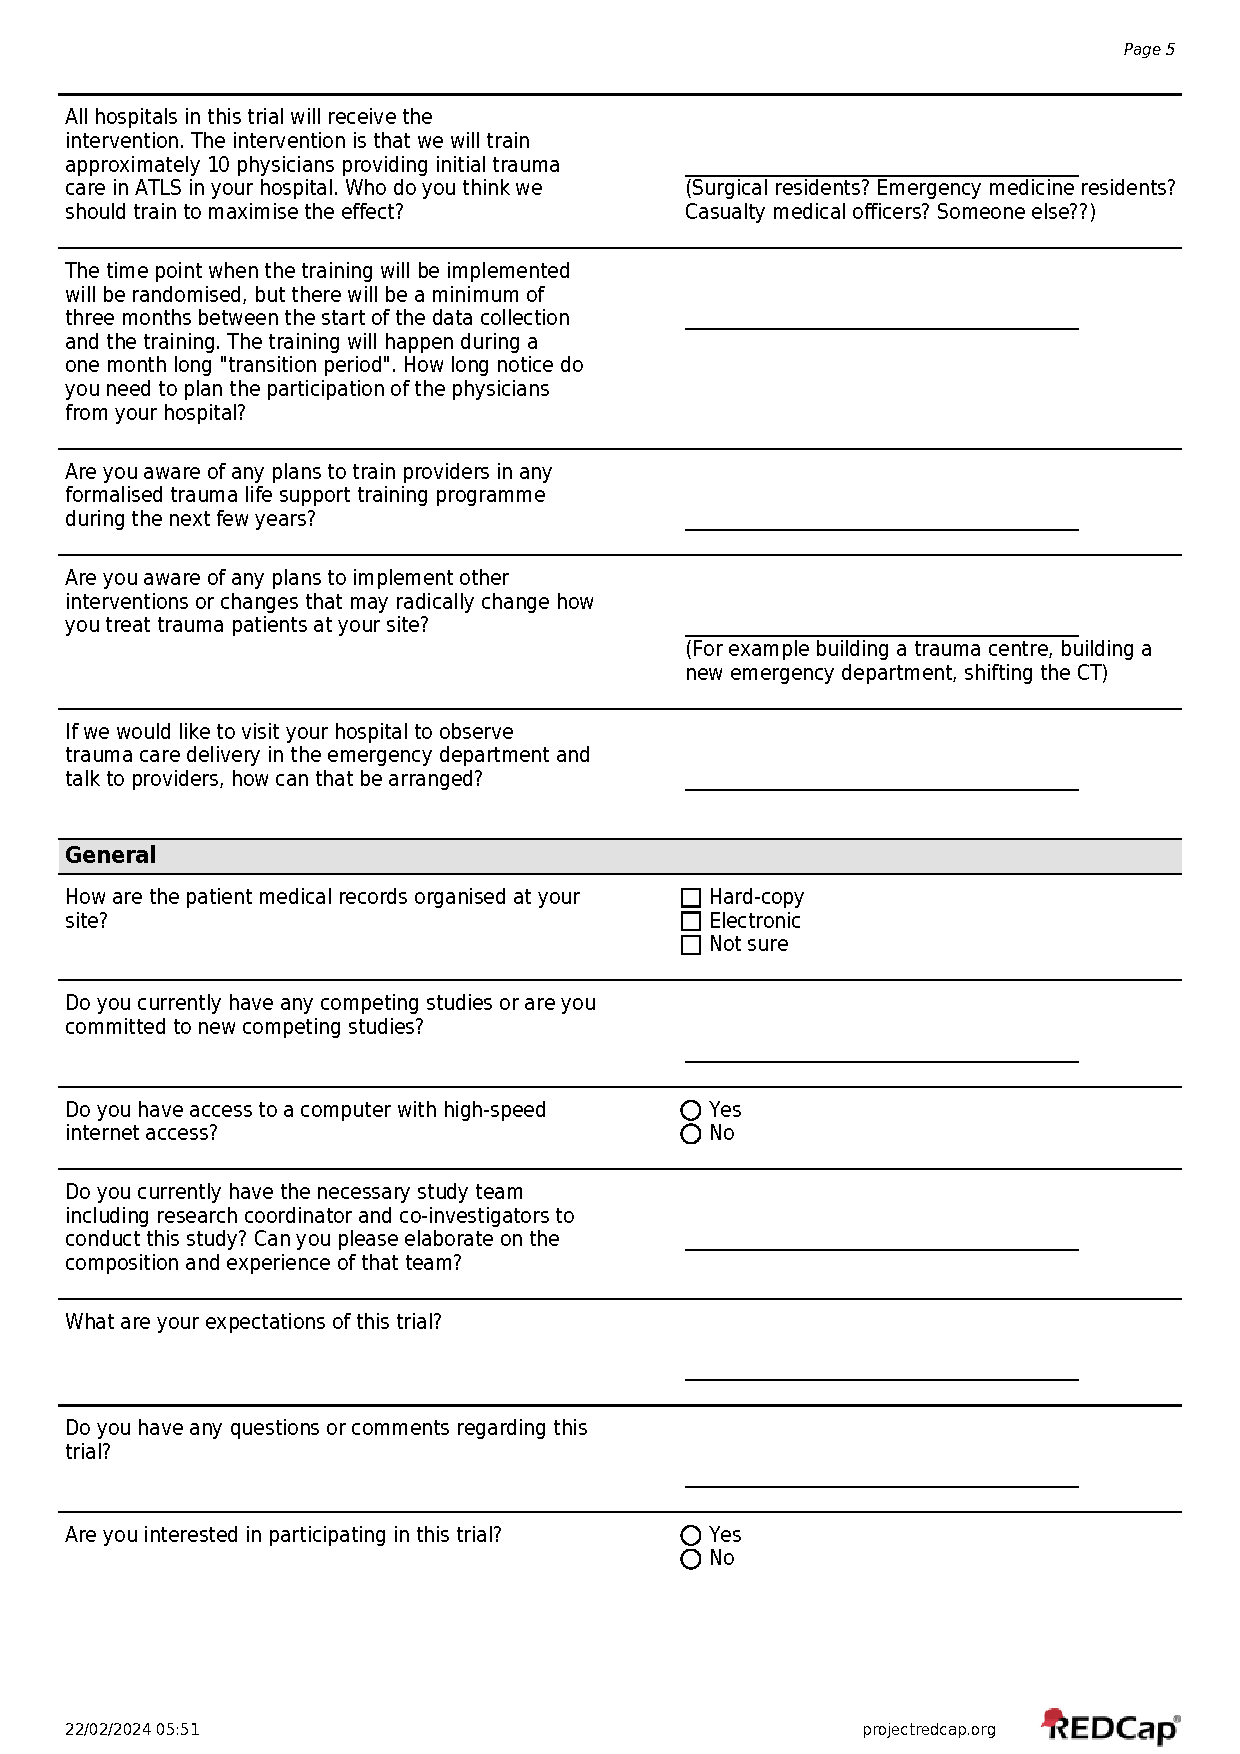
\includegraphics{./appendices/hospital-screening-interview-instrument/hospital-screening-interview-5.pdf}


\includegraphics{./appendices/hospital-screening-interview-instrument/hospital-screening-interview-6.pdf}

\hypertarget{sec-appendix-case-record-form}{%
\subsection{Case Record Form}\label{sec-appendix-case-record-form}}

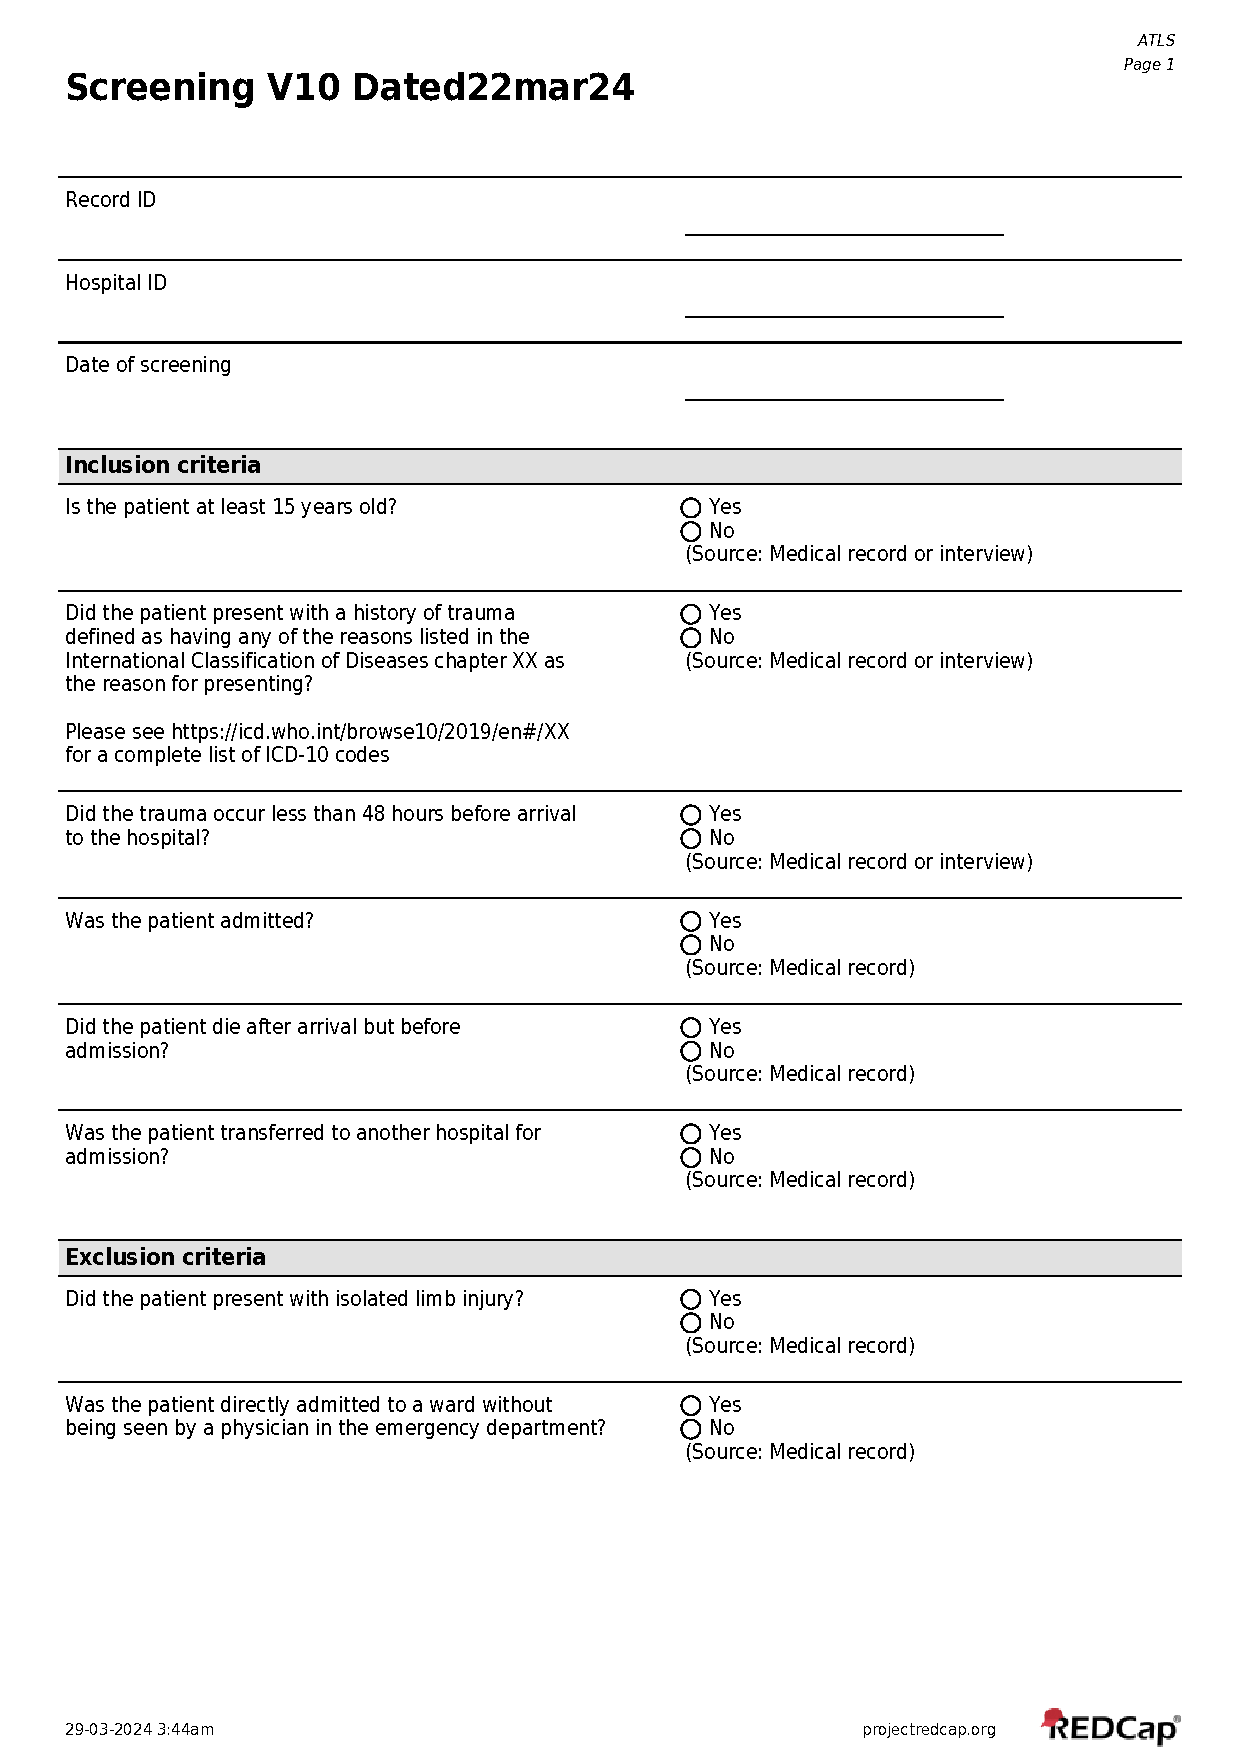
\includegraphics{../case-record-form/instrument-pdfs/pages/all-instruments-1.pdf}


\includegraphics{../case-record-form/instrument-pdfs/pages/all-instruments-2.pdf}

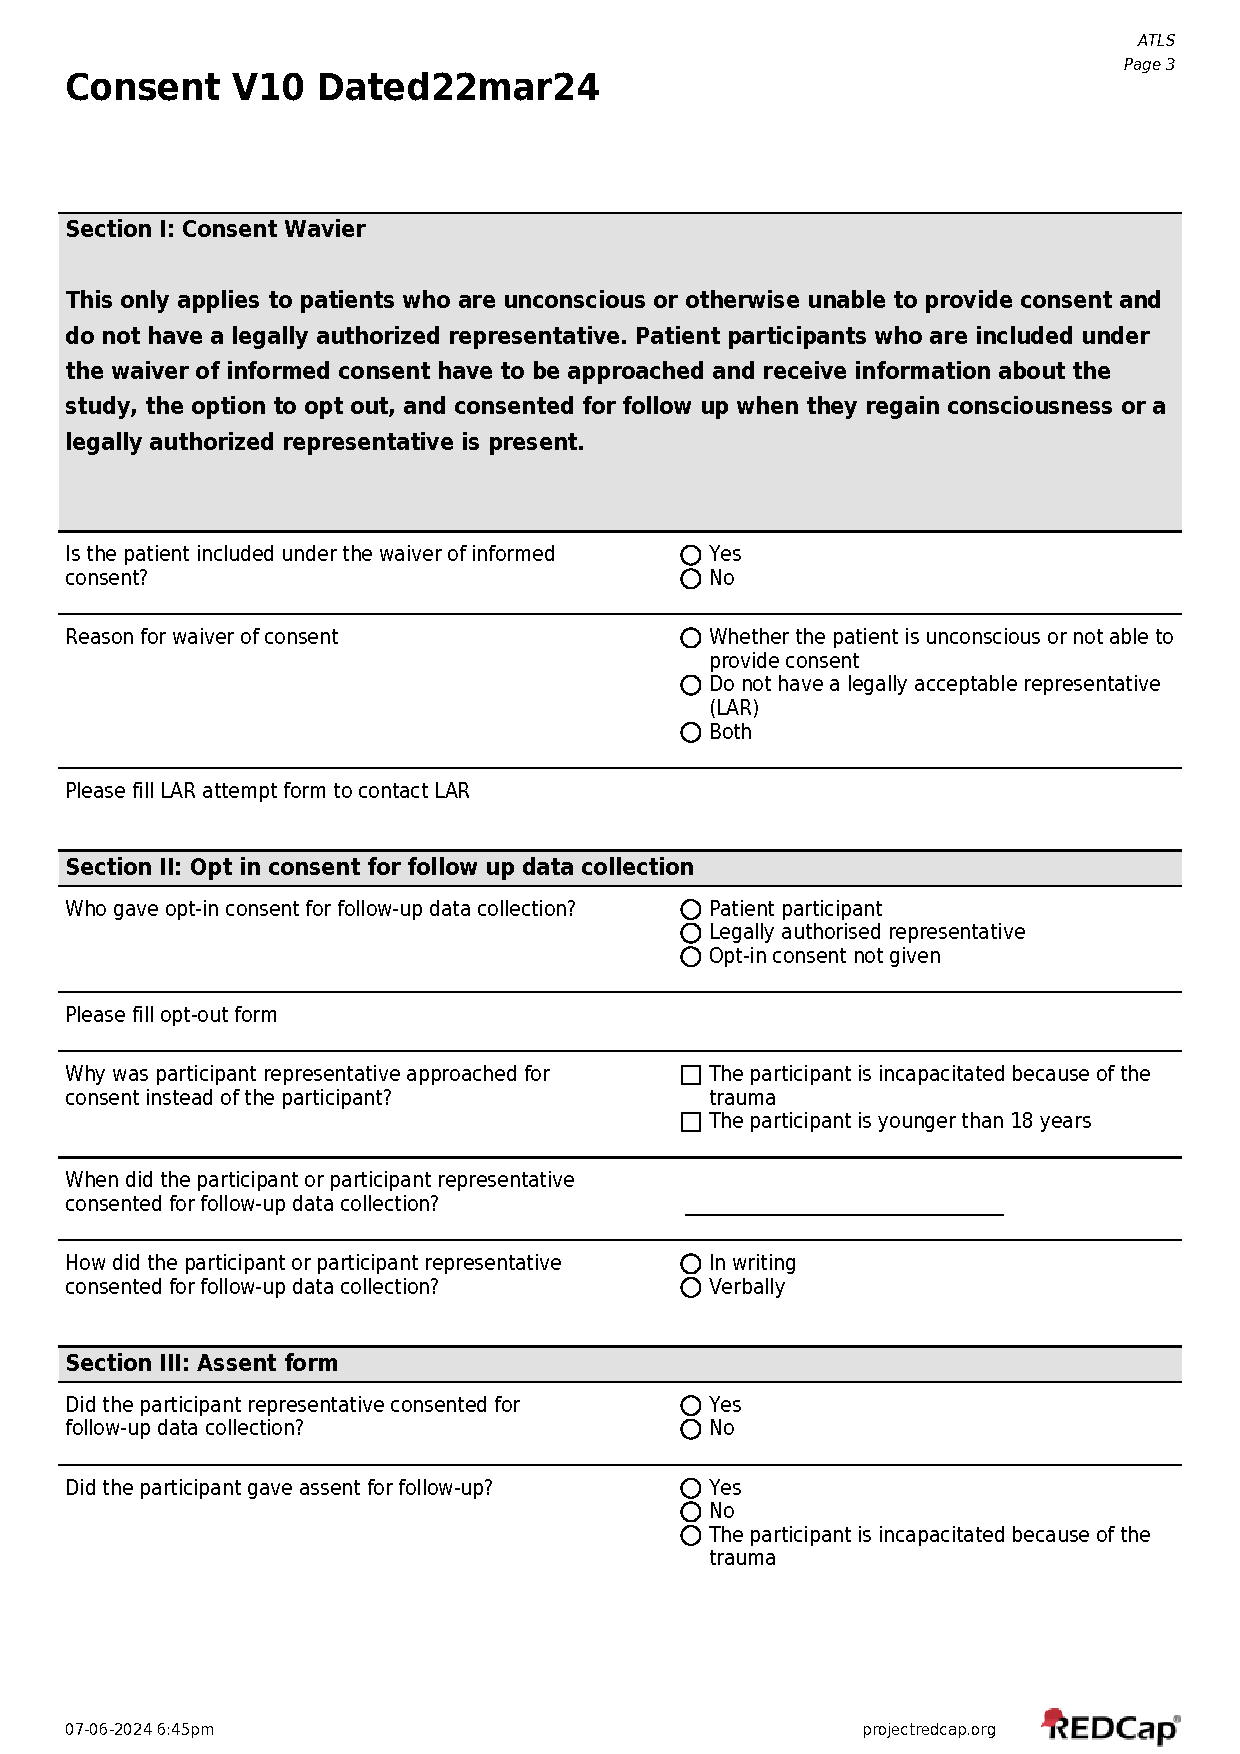
\includegraphics{../case-record-form/instrument-pdfs/pages/all-instruments-3.pdf}


\includegraphics{../case-record-form/instrument-pdfs/pages/all-instruments-4.pdf}


\includegraphics{../case-record-form/instrument-pdfs/pages/all-instruments-5.pdf}

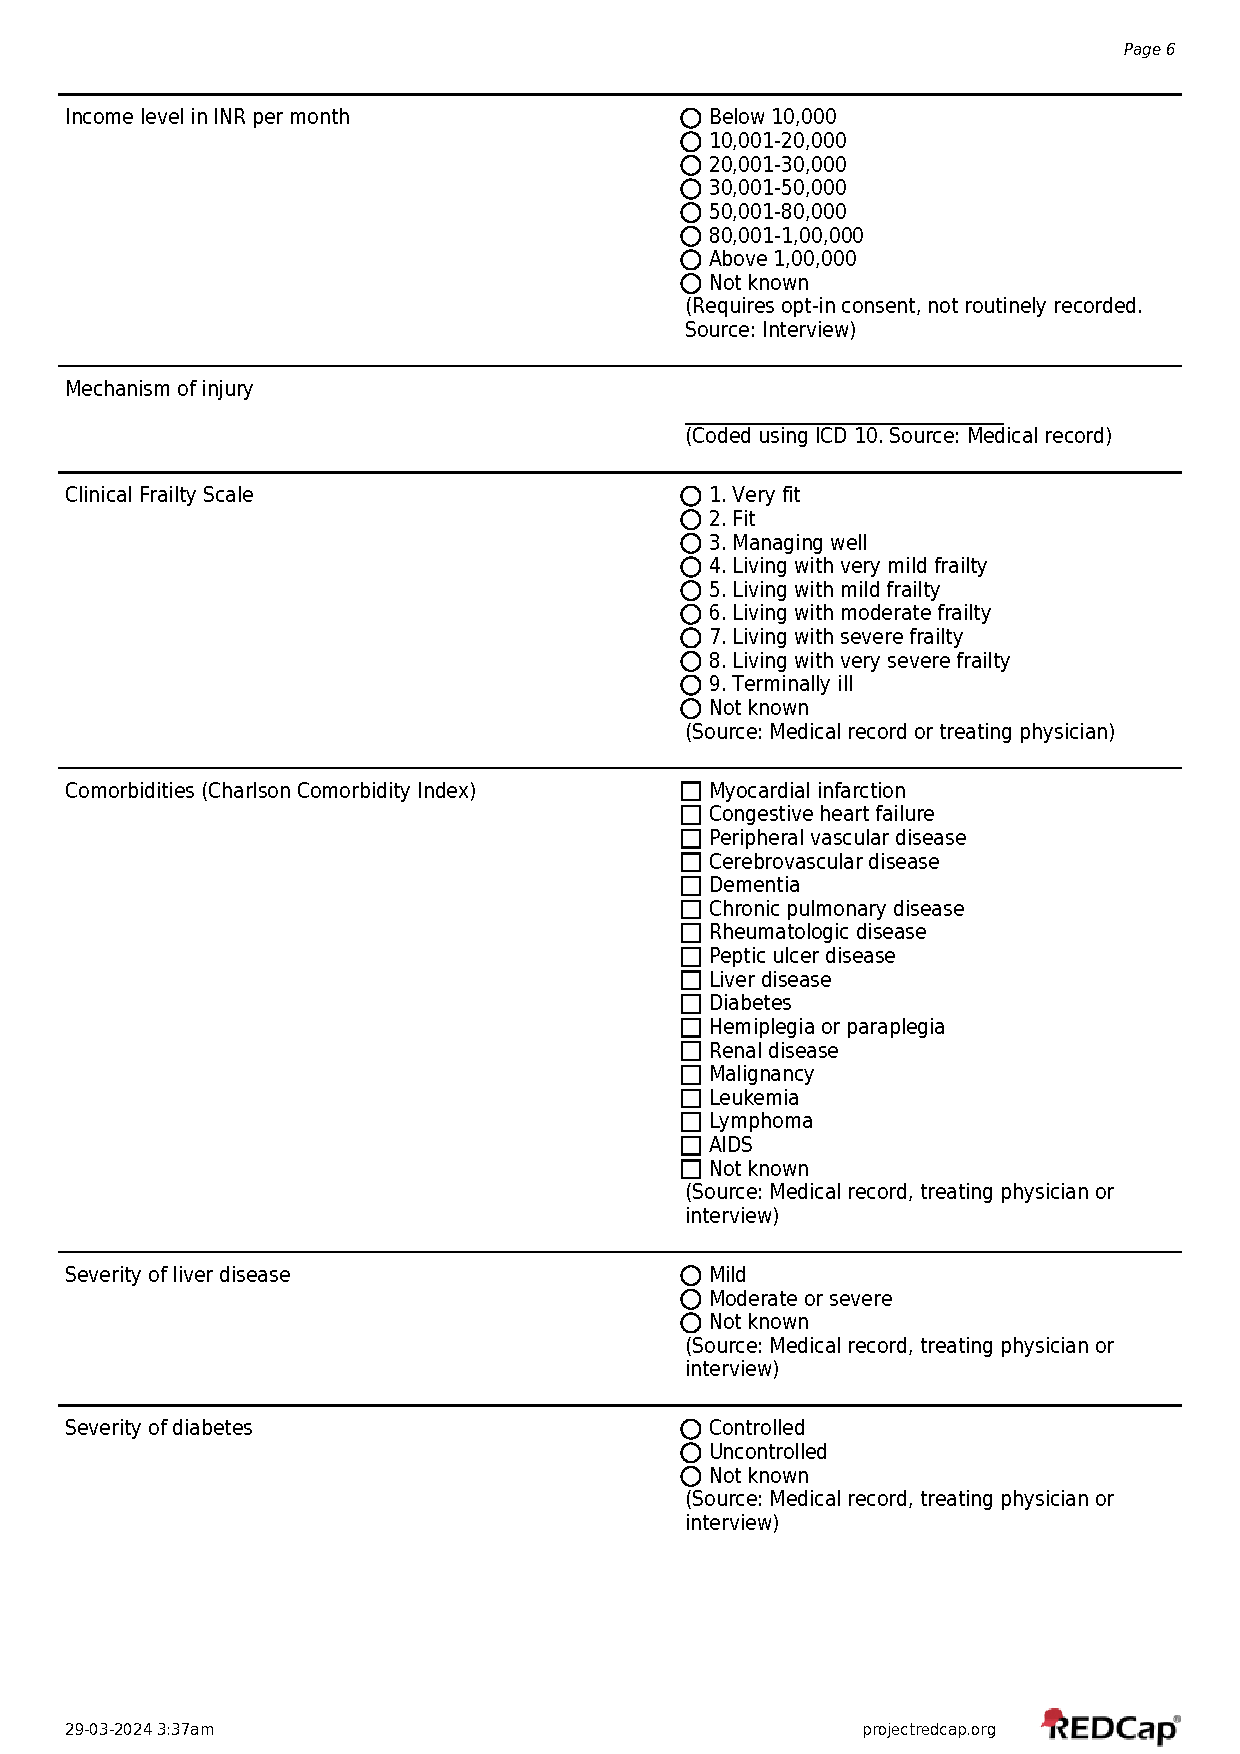
\includegraphics{../case-record-form/instrument-pdfs/pages/all-instruments-6.pdf}

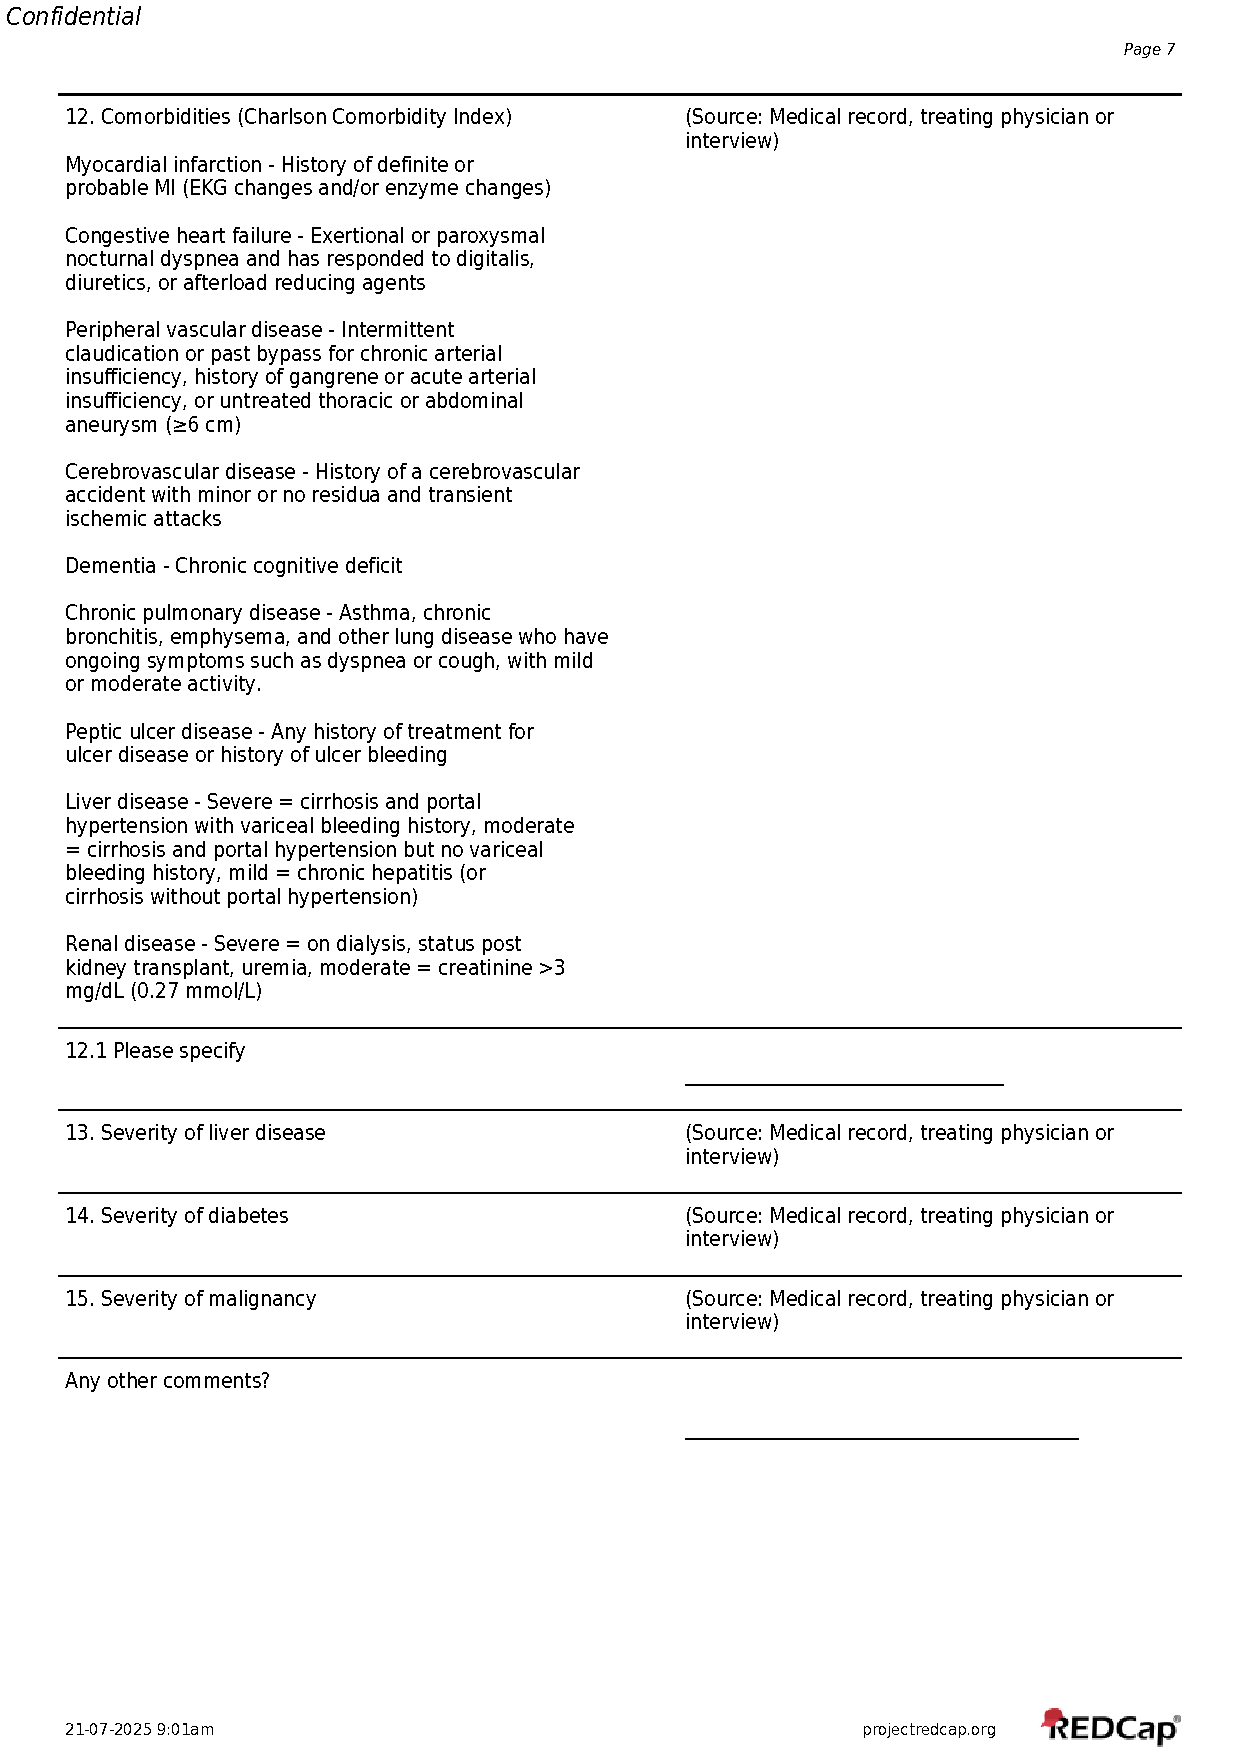
\includegraphics{../case-record-form/instrument-pdfs/pages/all-instruments-7.pdf}

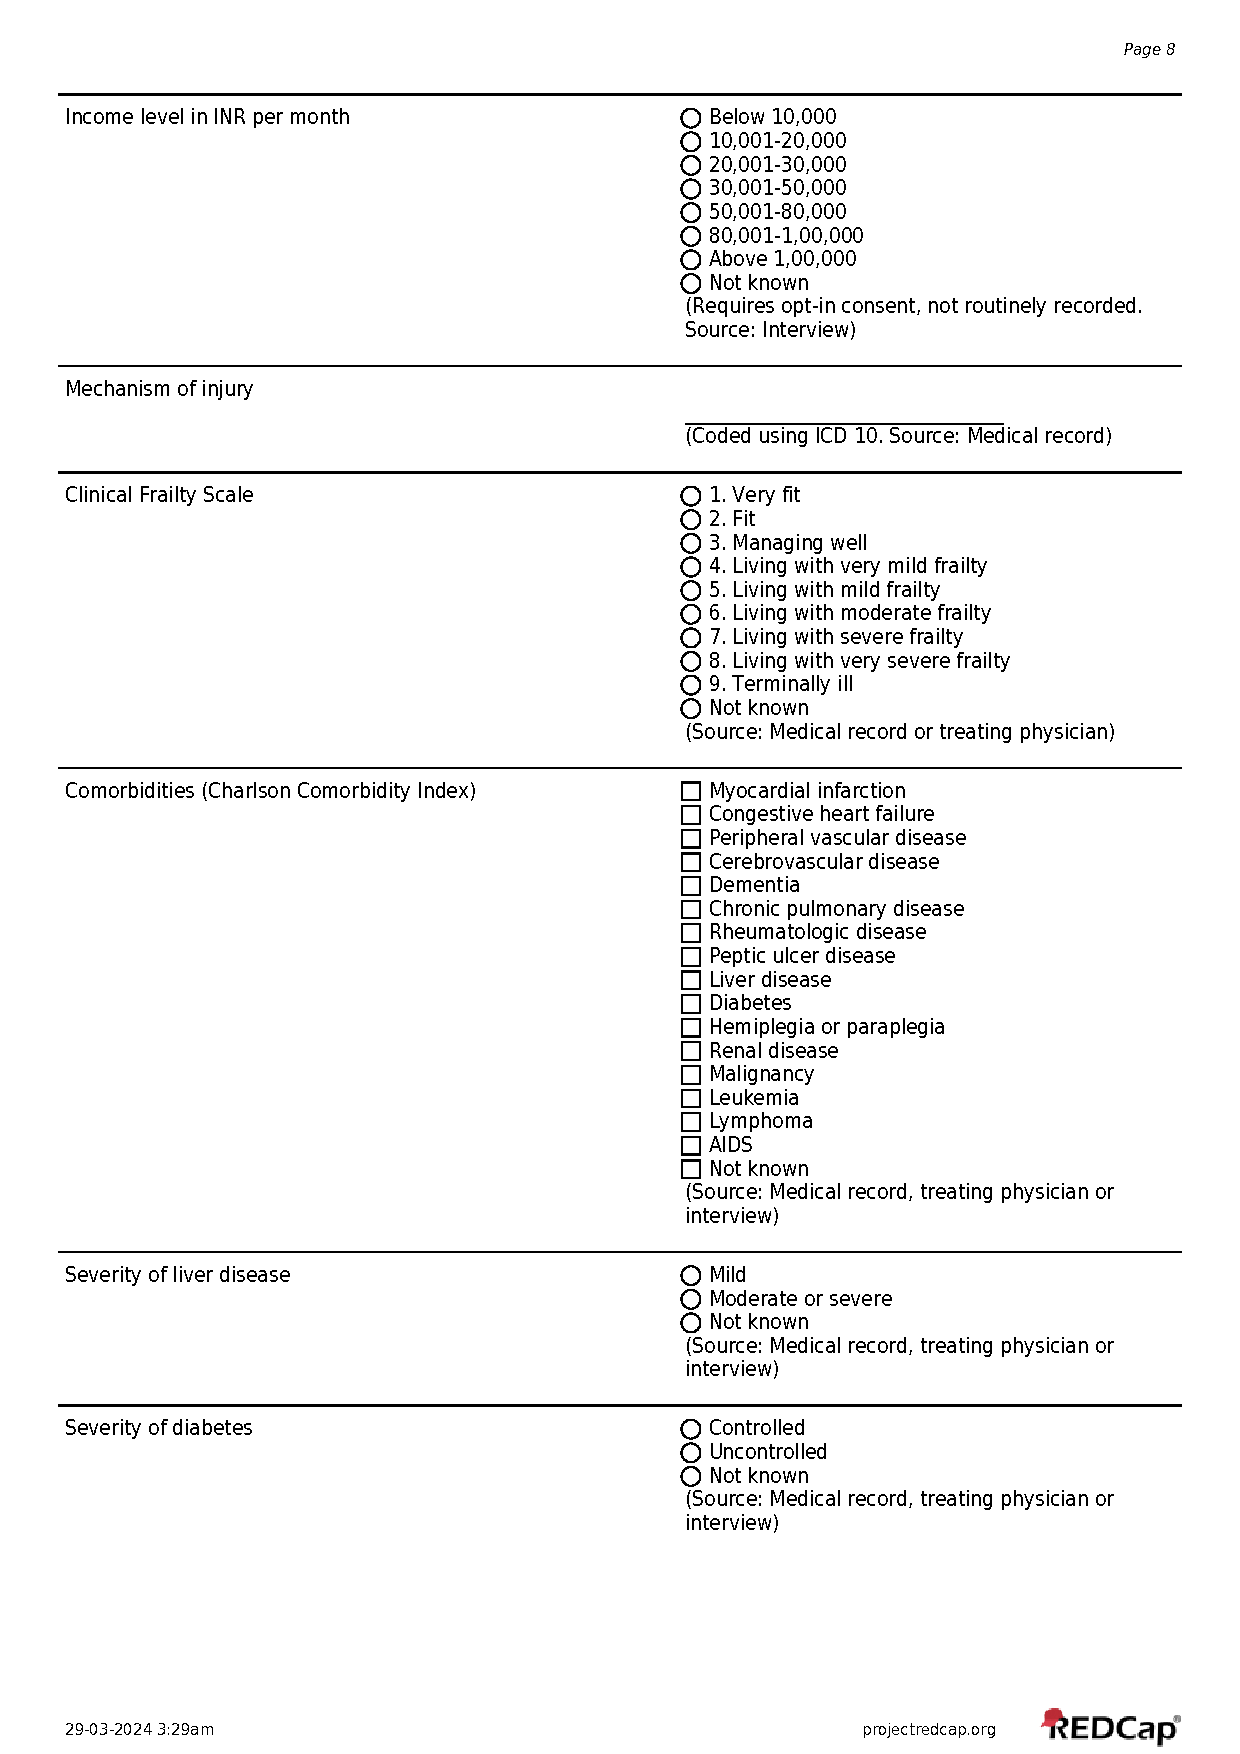
\includegraphics{../case-record-form/instrument-pdfs/pages/all-instruments-8.pdf}


\includegraphics{../case-record-form/instrument-pdfs/pages/all-instruments-9.pdf}

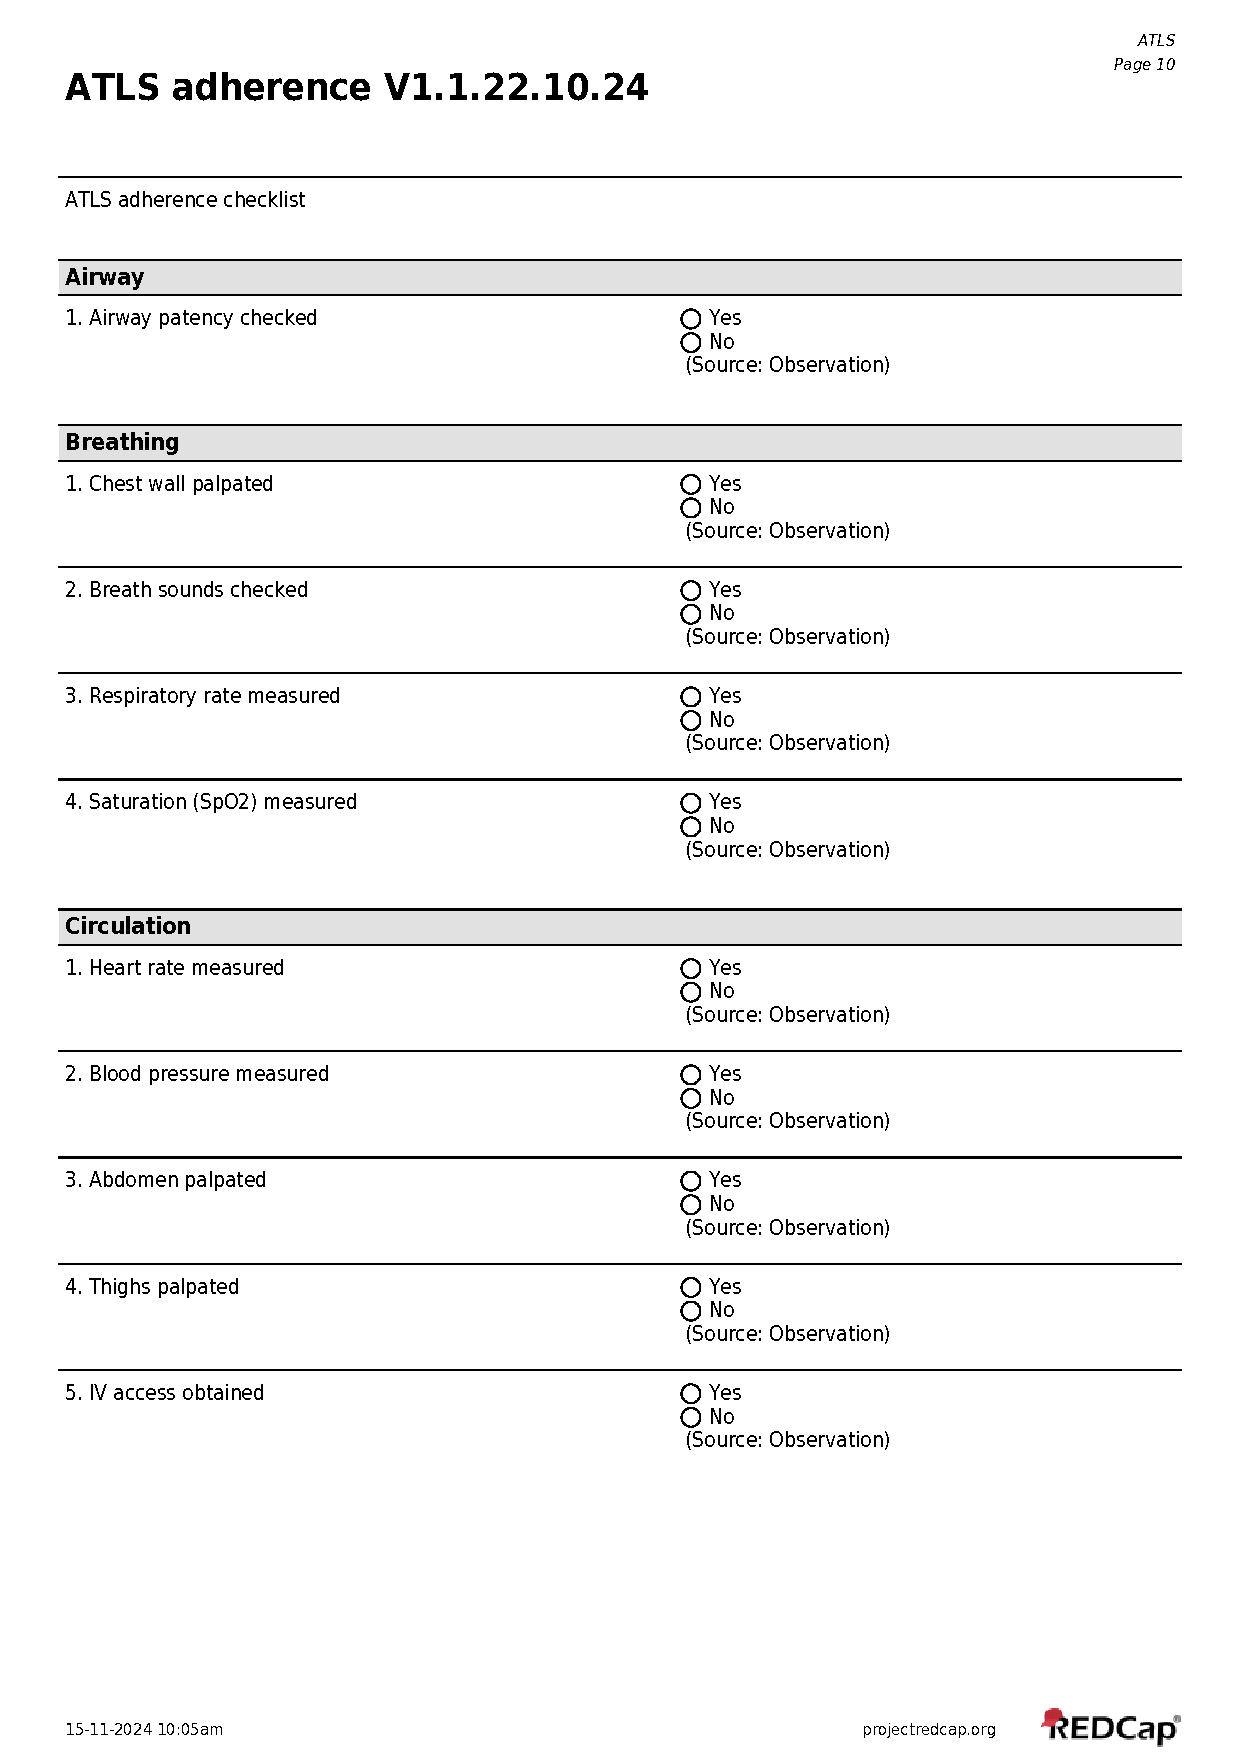
\includegraphics{../case-record-form/instrument-pdfs/pages/all-instruments-10.pdf}

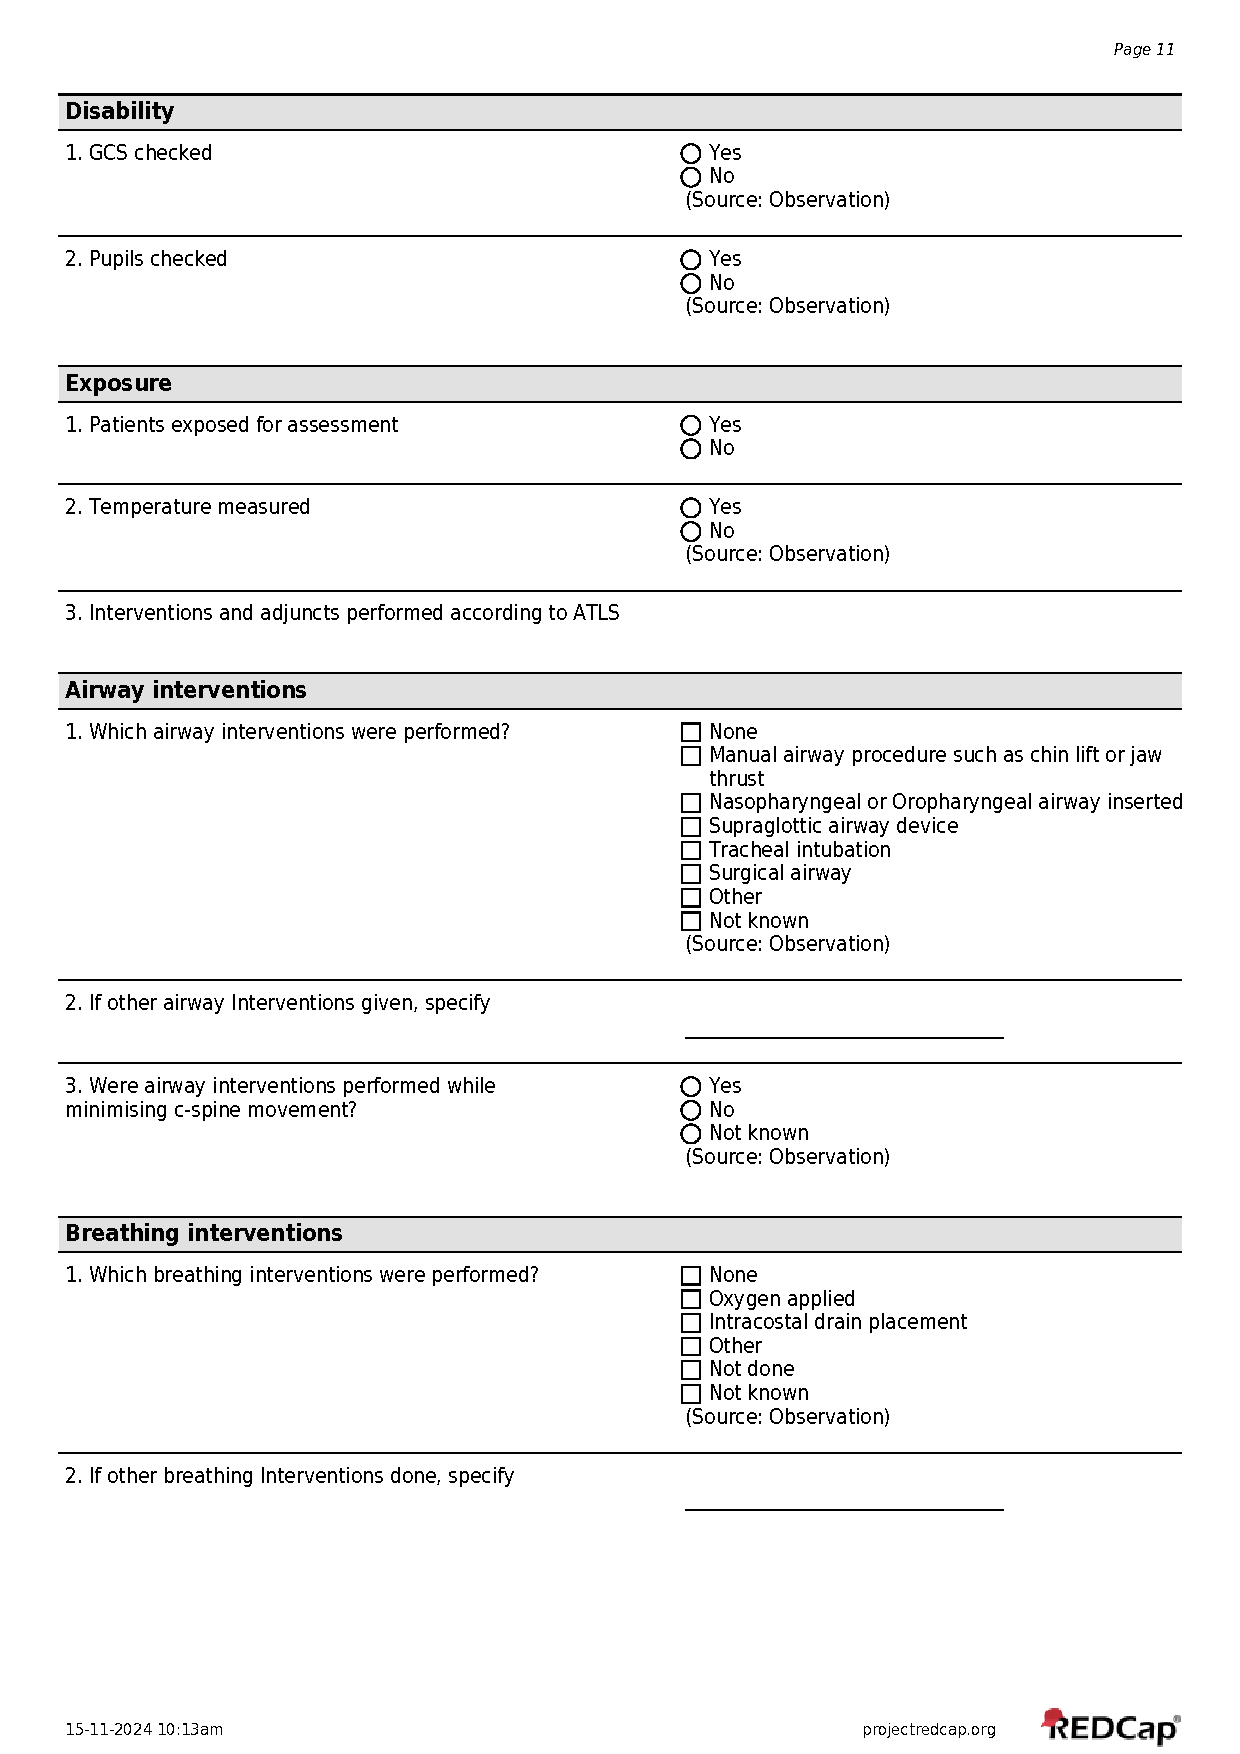
\includegraphics{../case-record-form/instrument-pdfs/pages/all-instruments-11.pdf}

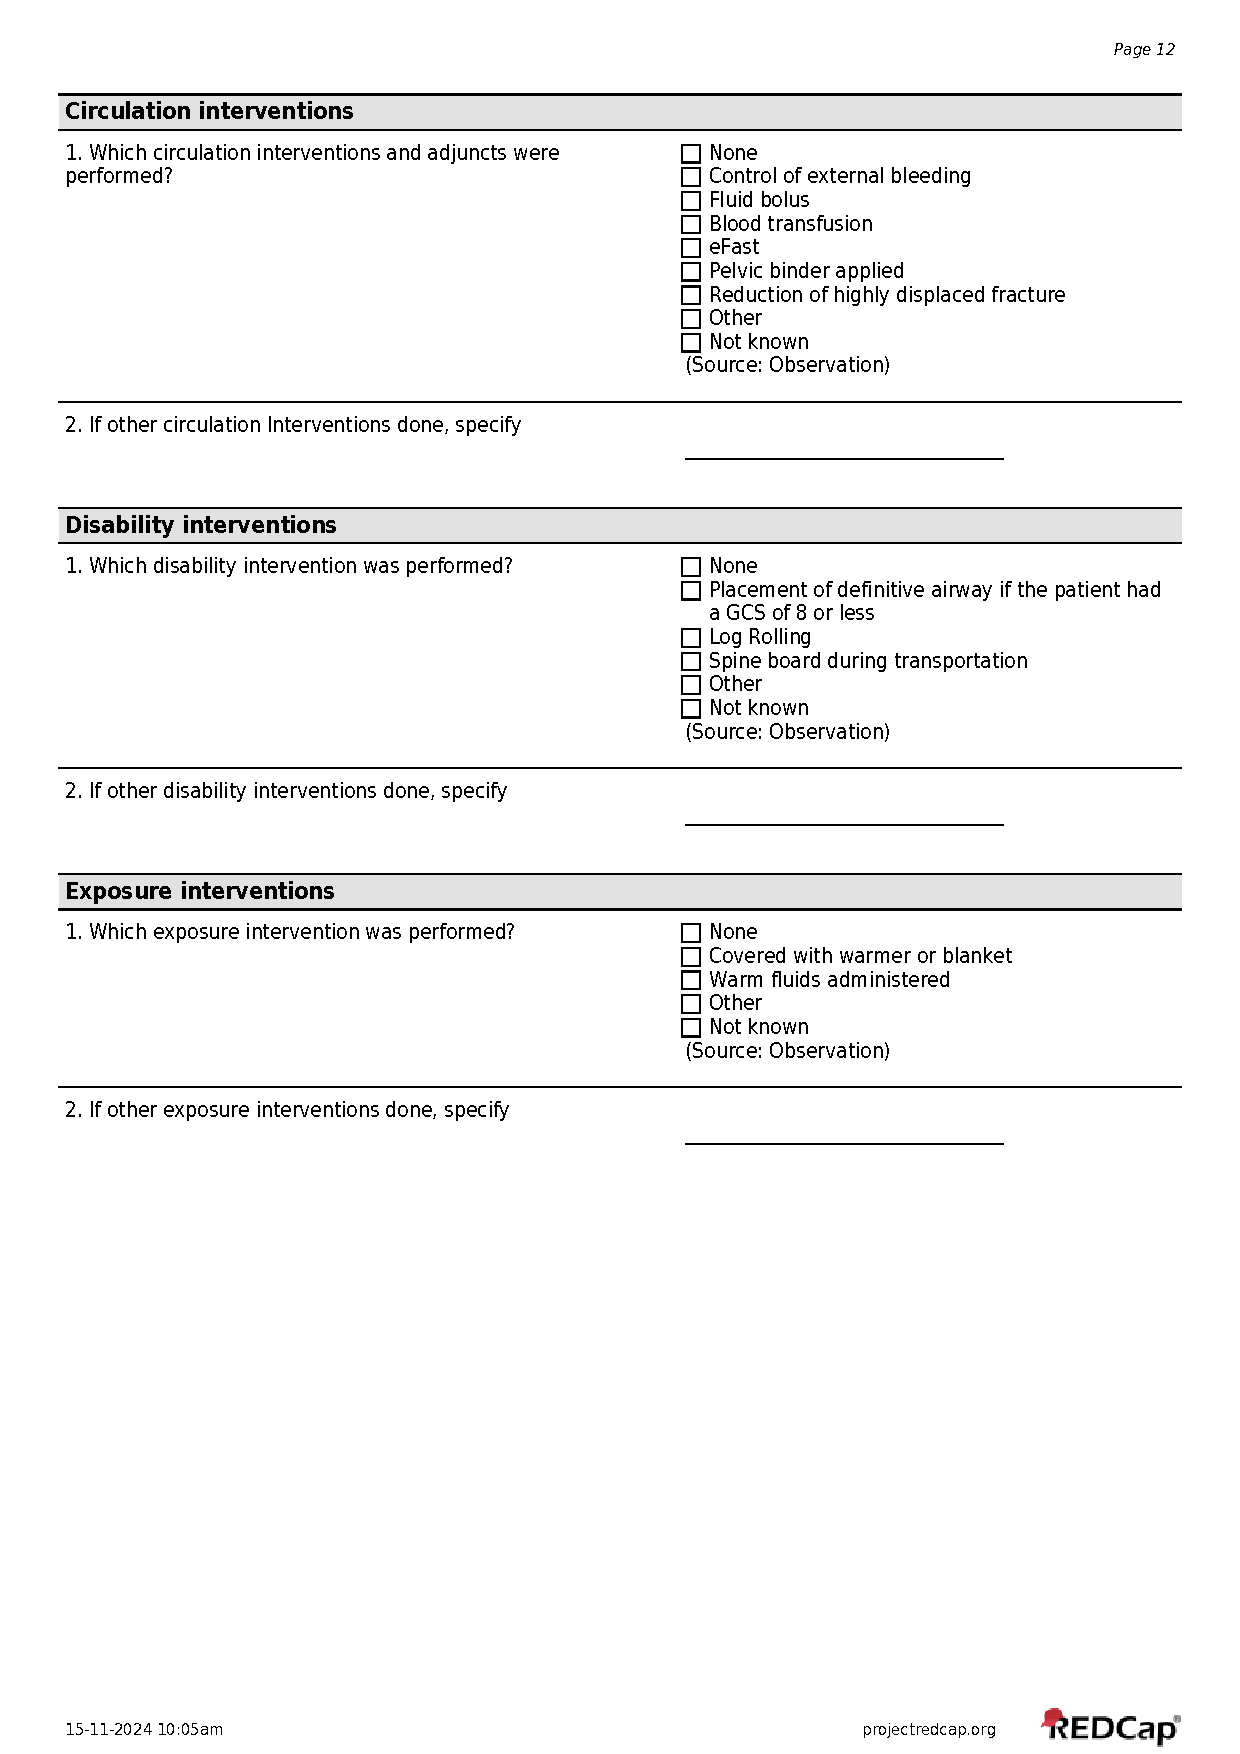
\includegraphics{../case-record-form/instrument-pdfs/pages/all-instruments-12.pdf}

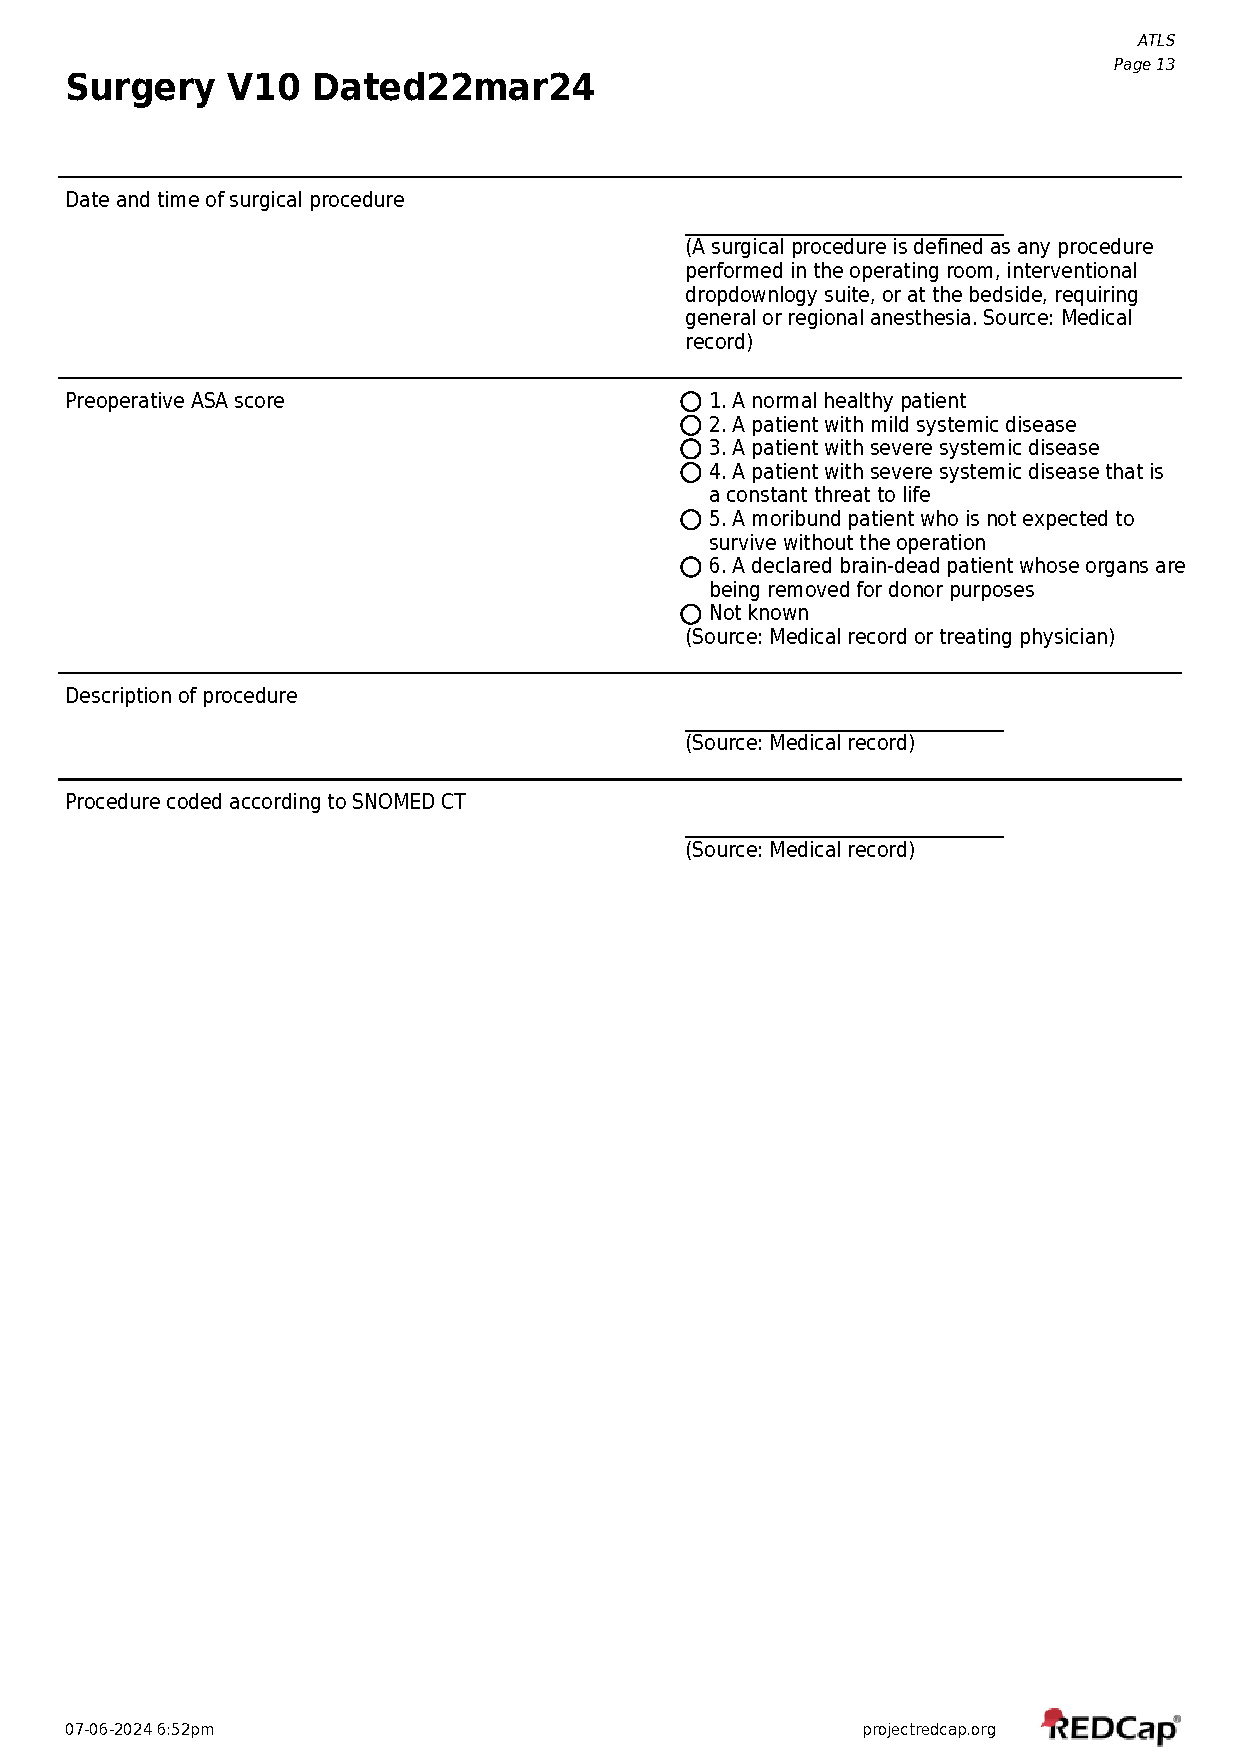
\includegraphics{../case-record-form/instrument-pdfs/pages/all-instruments-13.pdf}

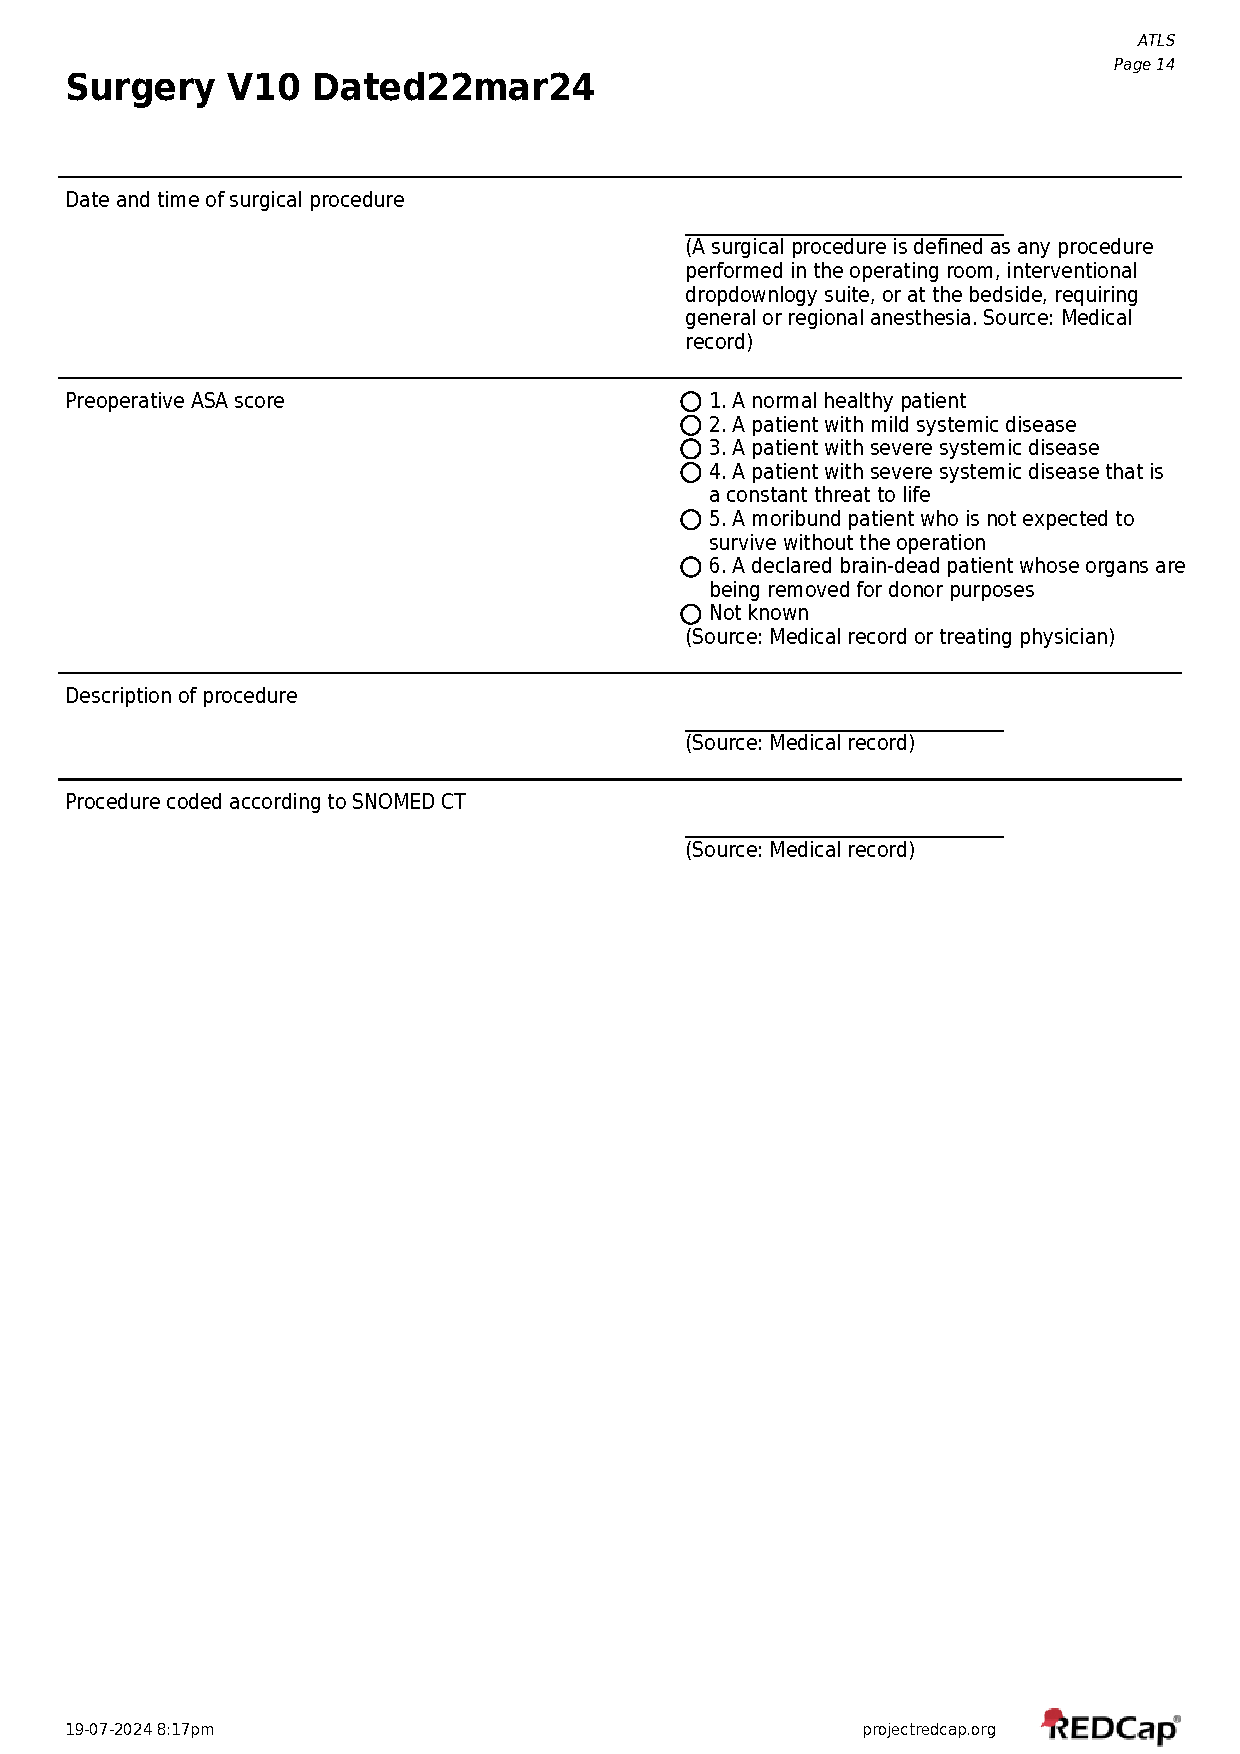
\includegraphics{../case-record-form/instrument-pdfs/pages/all-instruments-14.pdf}

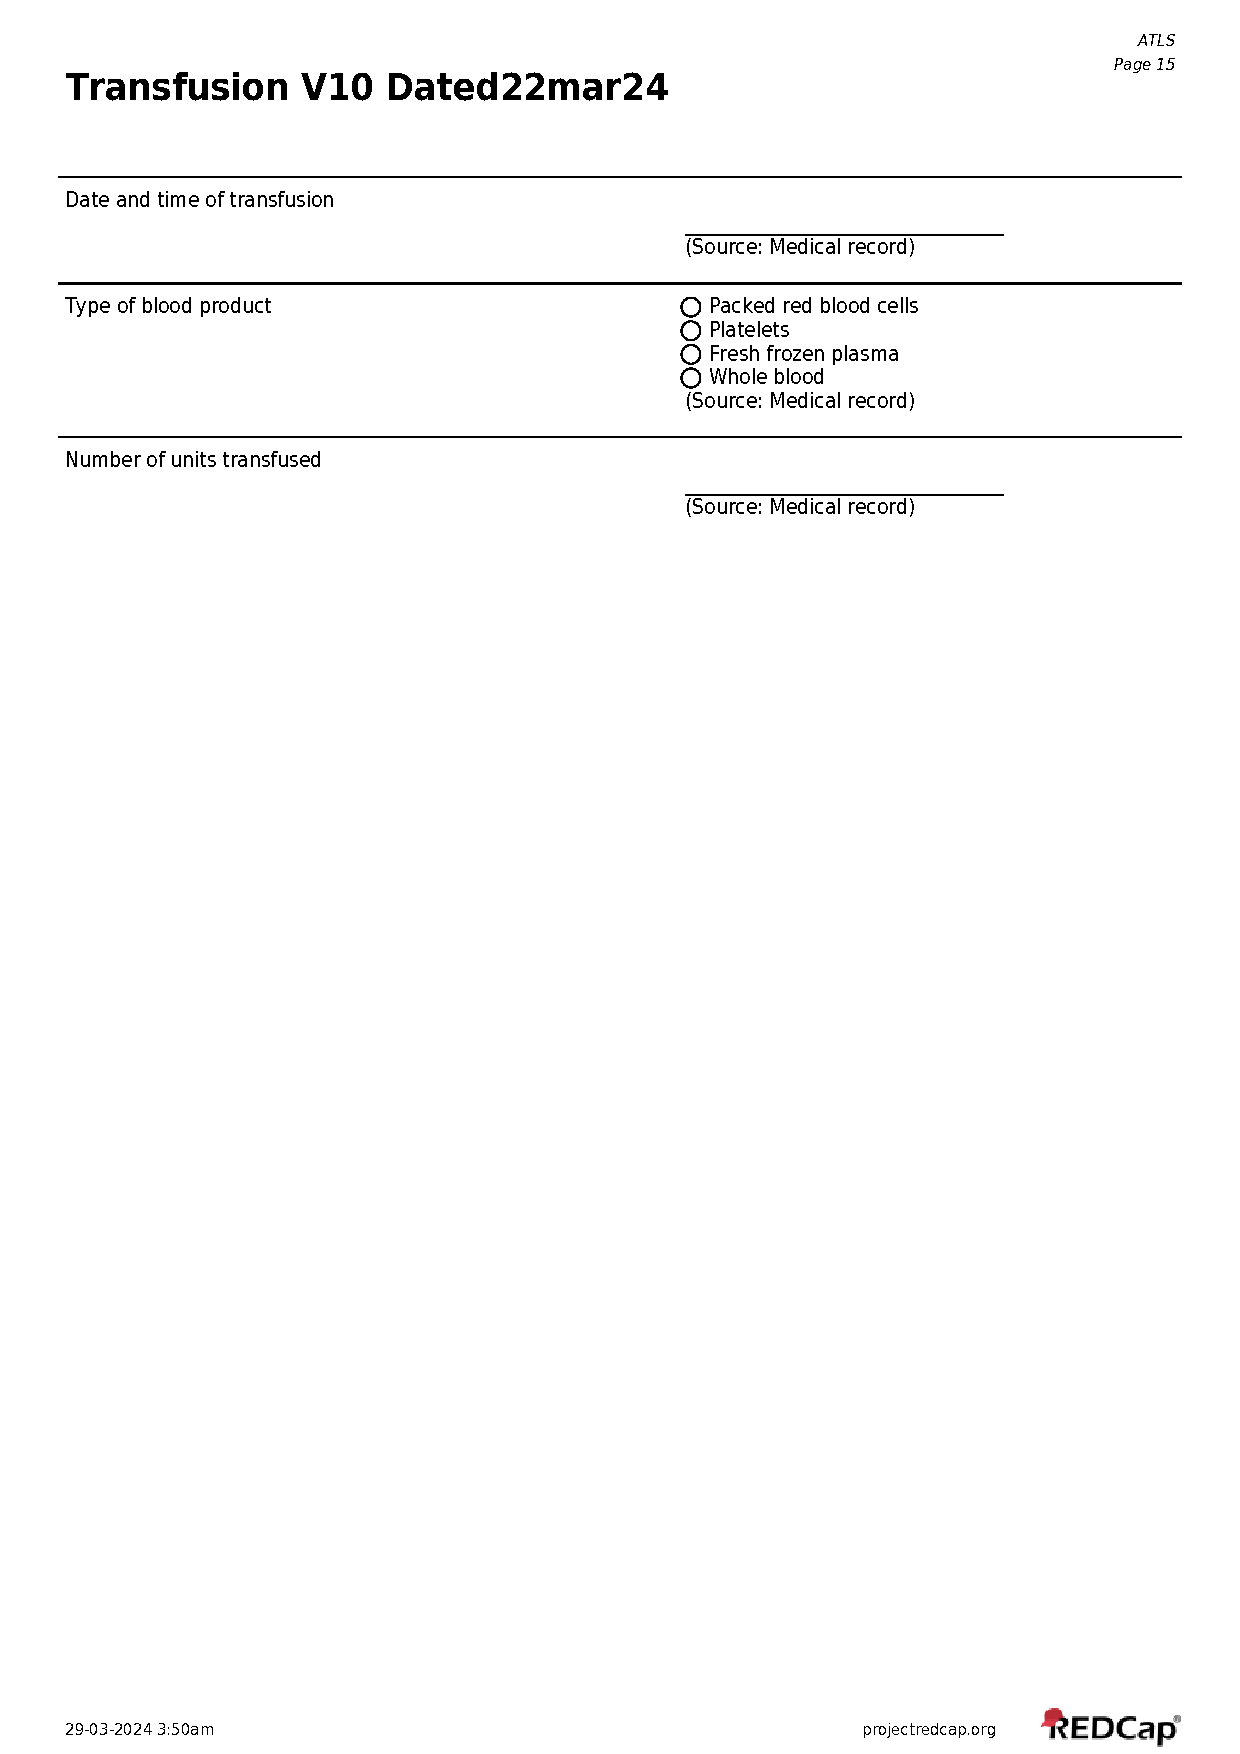
\includegraphics{../case-record-form/instrument-pdfs/pages/all-instruments-15.pdf}

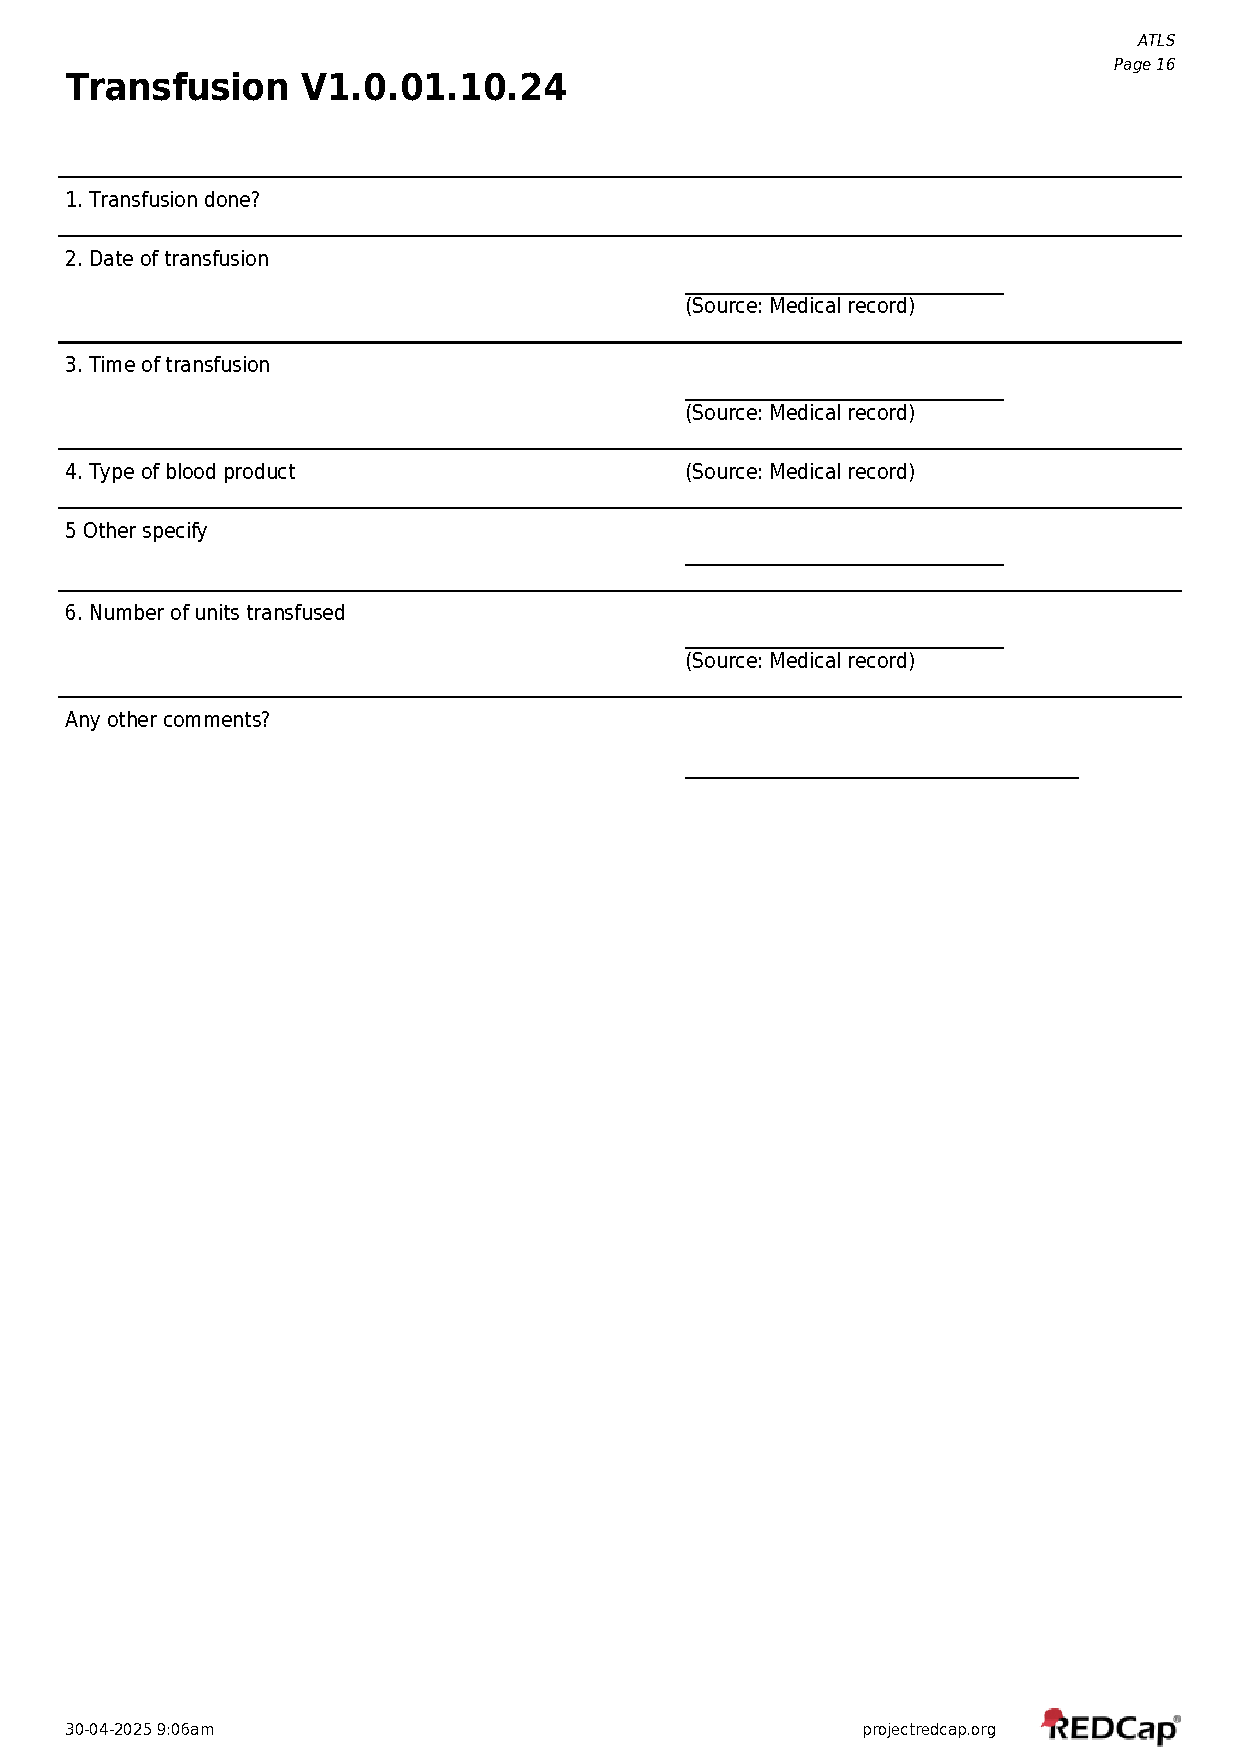
\includegraphics{../case-record-form/instrument-pdfs/pages/all-instruments-16.pdf}

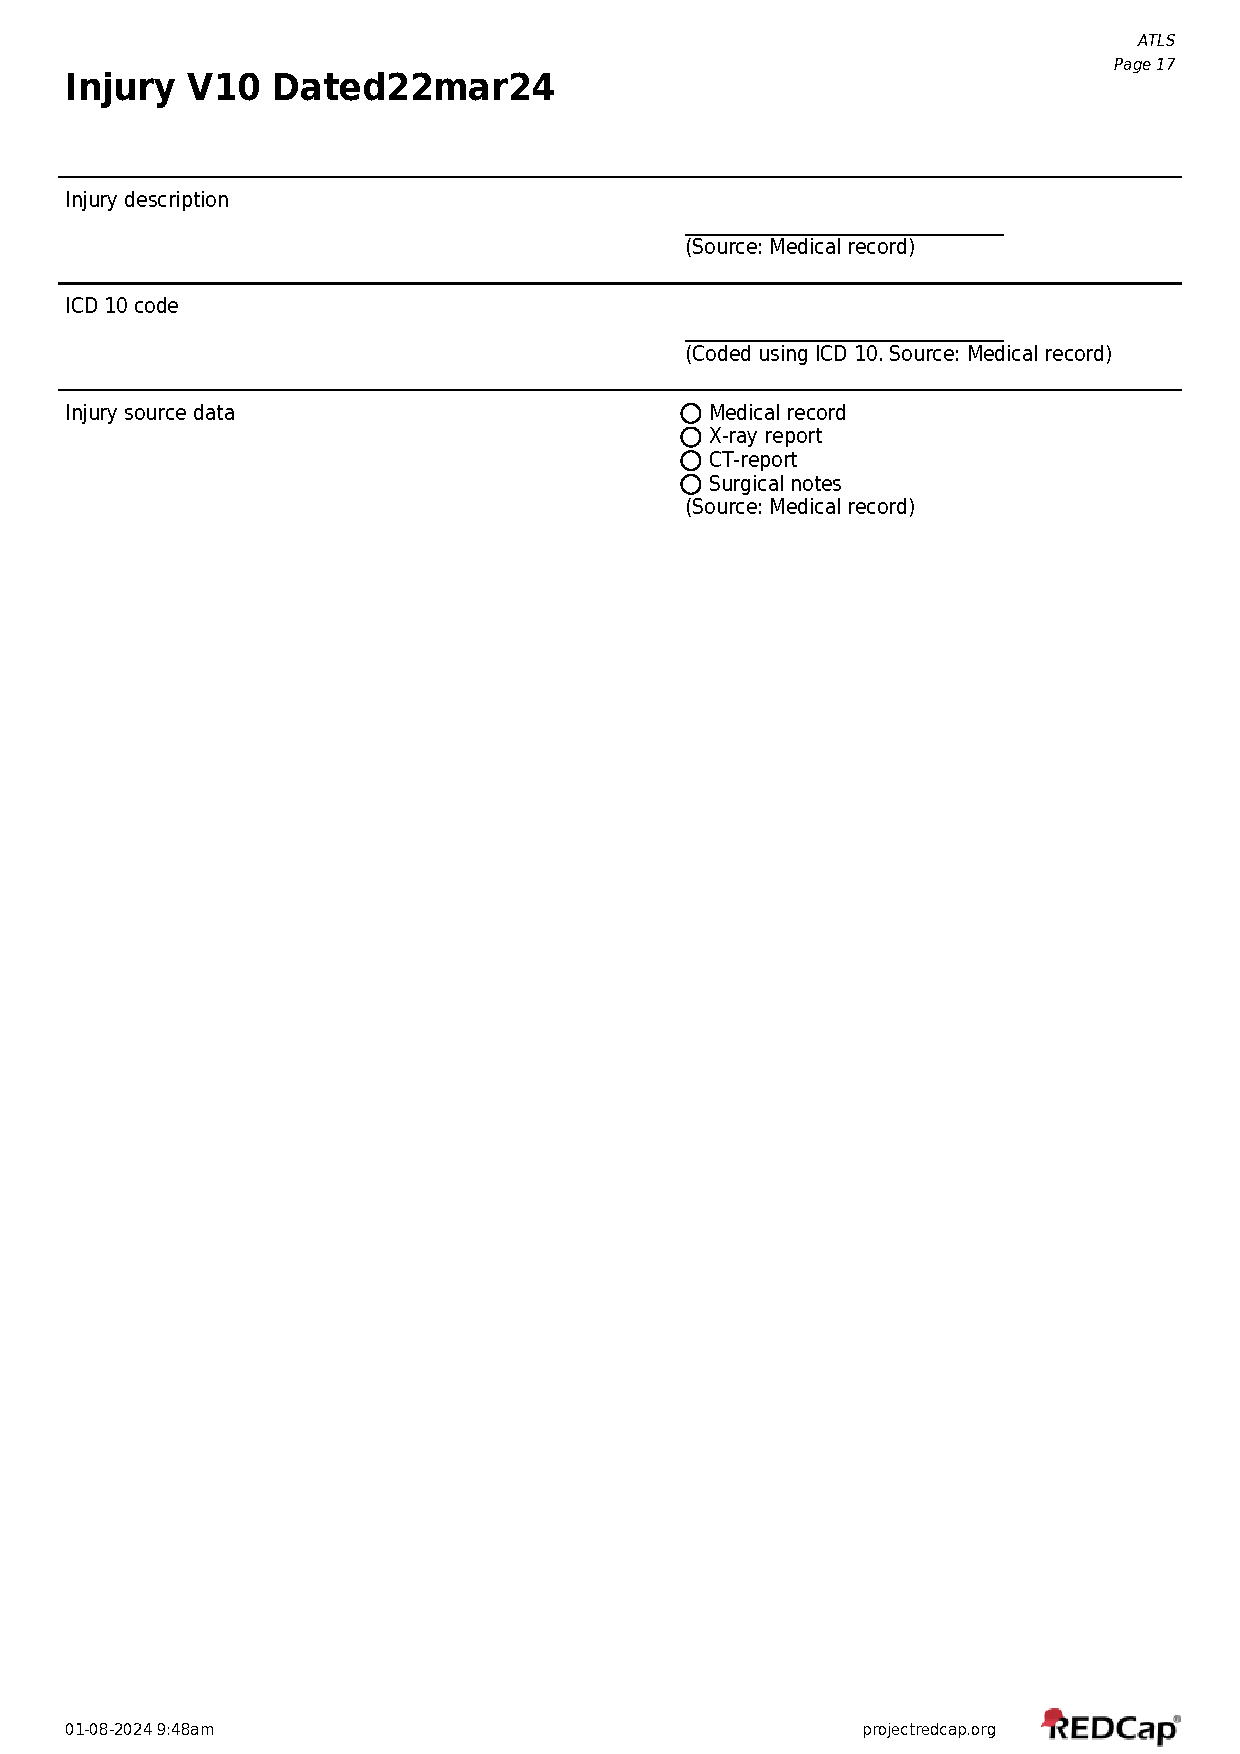
\includegraphics{../case-record-form/instrument-pdfs/pages/all-instruments-17.pdf}

\includegraphics{../case-record-form/instrument-pdfs/pages/all-instruments-18.pdf}

\includegraphics{../case-record-form/instrument-pdfs/pages/all-instruments-19.pdf}

\includegraphics{../case-record-form/instrument-pdfs/pages/all-instruments-20.pdf}

\includegraphics{../case-record-form/instrument-pdfs/pages/all-instruments-21.pdf}

\includegraphics{../case-record-form/instrument-pdfs/pages/all-instruments-22.pdf}

\includegraphics{../case-record-form/instrument-pdfs/pages/all-instruments-23.pdf}

\includegraphics{../case-record-form/instrument-pdfs/pages/all-instruments-24.pdf}

\includegraphics{../case-record-form/instrument-pdfs/pages/all-instruments-25.pdf}

\includegraphics{../case-record-form/instrument-pdfs/pages/all-instruments-26.pdf}

\includegraphics{../case-record-form/instrument-pdfs/pages/all-instruments-27.pdf}

\includegraphics{../case-record-form/instrument-pdfs/pages/all-instruments-28.pdf}

\includegraphics{../case-record-form/instrument-pdfs/pages/all-instruments-29.pdf}

\includegraphics{../case-record-form/instrument-pdfs/pages/all-instruments-30.pdf}

\includegraphics{../case-record-form/instrument-pdfs/pages/all-instruments-31.pdf}

\includegraphics{../case-record-form/instrument-pdfs/pages/all-instruments-32.pdf}



\end{document}
